\documentclass[openany,
ngerman,
toc=flat,
toc=chapterentrywithdots,
captions=tableabove,
listof=entryprefix,
listof=leveldown,
fontsize=12pt,
numbers=noenddot]
{book}
\usepackage{blindtext}
\usepackage{xcolor}
\usepackage{amsfonts}
\usepackage{hyperref} 
\usepackage{subcaption}
\usepackage{indentfirst}
\usepackage{graphicx}
\usepackage[normalem]{ulem}
\usepackage [english]{babel}
\usepackage [autostyle, english = american]{csquotes}
\usepackage{appendix}
\usepackage{tabularx}
\usepackage{bbm}
\usepackage{amsmath,amssymb}
\usepackage{mathtools}
\usepackage{makecell}
\graphicspath{ {./images/} }
\usepackage{enumitem}
\usepackage{soul}
\usepackage{mathtools}
\usepackage{wrapfig}
\usepackage{mathrsfs}
\usepackage{MnSymbol,wasysym}
\usepackage{centernot}
\usepackage{amsthm}
\usepackage{biblatex}
\addbibresource{citations.bib}
\allowdisplaybreaks

\MakeOuterQuote{"}

\newtheorem{theorem}{Theorem}[chapter]
\newtheorem*{theorem*}{Theorem}
\newtheorem{definition}[theorem]{Definition}
\newtheorem{conjecture}[theorem]{Conjecture}
\newtheorem{corollary}[theorem]{Corollary}
\newtheorem{lemma}[theorem]{Lemma}
\newtheorem*{lemma*}{Lemma}
\newtheorem{proposition}[theorem]{Proposition}
\newtheorem{example}[theorem]{Example}
\newenvironment{remark}[1][Remark:]{\begin{trivlist}
		\item[\hskip \labelsep {\bfseries #1}]}{\end{trivlist}}

\newcommand{\defeq}{\mathrel{\mathop:}=}
\newcommand{\stackeq}[1]{\stackrel{\mathclap{\normalfont\mbox{\normalfont\tiny {#1}}}}{=}}
\newcommand{\stackon}[2]{\stackrel{\mathclap{\normalfont\mbox{\normalfont\tiny {#1}}}}{#2}}
\newcommand\reals{\mathbb{R}}
\newcommand\field{\mathbb{F}}
\newcommand\complex{\mathbb{C}}
\newcommand\schwartz{\mathcal{S}}
\renewcommand{\mod}{ \textrm{ mod }}
\newcommand\naturals{\mathbb{N}}
\usepackage{geometry}
\geometry{
	letterpaper,
	margin=1in
}
\usepackage{blindtext}
\usepackage{tikz,tcolorbox,tikz-3dplot}
\usepackage{pgfplots}
\usepgfplotslibrary{fillbetween}
\usepackage{xcolor}
\usepackage{amsfonts}
\usepackage{hyperref} 
\usepackage{indentfirst}
\usepackage{graphicx}
\usepackage{caption}
\usepackage{subcaption}
\usepackage[normalem]{ulem}
\usepackage [english]{babel}
\usepackage [autostyle, english = american]{csquotes}
\usepackage{appendix}

\usepackage[ruled,linesnumbered]{algorithm2e}
\SetKwComment{Comment}{/* }{ */}
\DontPrintSemicolon 
\usepackage{tabularx}
\usepackage{amsmath,amssymb}
\usepackage{mathtools}
\usepackage{makecell}
\graphicspath{ {./images/} }
\usepackage{enumitem}
\usepackage{soul}
\usepackage{mathtools}
\usepackage{wrapfig}
\usepackage{mathrsfs}
\usepackage{centernot}
\usepackage{amsthm}
\usepackage{listings}
\setcounter{chapter}{-1}
\title{Large values of Dirichlet Polynomials and Zero Density Results of the Riemann Zeta function}
\author{Yung Chi Li}
%\date{January 2024}
\usepackage{titling}
\predate{}
\postdate{}
\date{}
\usepackage{tocloft}
\setlength{\cftaftertoctitleskip}{0.3em}
%\setlength{\cftbeforetoctitleskip}{1 em}
\begin{document}

%\maketitle
\begin{titlepage}
    \begin{center}
        \vspace*{1cm}
            
        \Large
        \textbf{Large values of Dirichlet Polynomials and Zero Density Results of the Riemann Zeta Function}
            
        \vspace{0.5cm}
        
        \Large
        Yung Chi Li
            
        \vfill
            
       	Submitted in partial fulfillment of the\\ requirements of
		Honors in Mathematics\\
		
		
		Northwestern University
            
    
            
    \end{center}
\end{titlepage}

\section*{Overview}
	We motivate the result of large values of Dirichlet polynomials through the study of primes in short intervals. We first introduce the Riemann Zeta function. We then prove the Prime Number Theorem to demonstrate the connection of Zeta zeros and primes, with the Riemann Hypothesis leading to the tightest bound on the error term of the Prime Number Theorem. 
	The Riemann Hypothesis has not be proved or disproved. Nevertheless, one can still obtain unconditional results on the error term through appealing to the distribution of Zeta zero density. We will provide the previous bound on the density of zeros and sketch its refinement. Finally, extending from the ideas of Guth and Maynard's proof in section 5, we provide a generalization for the analogous Hal\'asz inequality lemma for Dirichlet L-functions.


{\let\clearpage\relax \tableofcontents}
\section*{Statement Regarding Generative AI}
No part of this thesis had been aided by generative AI.

\section*{Acknowledgements}
I thank my advisor, Professor Maksym Radziwi\l\l, for his guidance on topic selection, explanation of current literature, and insights into solving hybrid Guth-Maynard. 
I also thank Vishal Gupta, who had been collaborating with me on the problem of generalizing the result of Guth and Maynard and provided key observations that allowed 
me to crack the $S_3$ term.
\chapter{Notation and Preliminaries}
\section*{Notation}
Below are the notational preferences of the author.
\begin{enumerate}
    \item $p$ always denotes a prime, and by extension $p_j,p_n$ etc.
\end{enumerate}

\section*{Preliminaries}
Here we provide some supplementary definitions and statements of theorems. These results are well-known. 
\subsection*{Number Theory}
\begin{definition}[Dirichlet Characters]
	\label{dcharacter}
	Let $q\in\naturals$. A Dirichlet character $\chi:\mathbb{N}\to\complex$ modulus $q$ is an arithmetic function satisfying \begin{itemize}
		\item \textit{(Periodicity)} $\chi(n+q)=\chi(n)\forall n\in\naturals$.
		\item \textit{(Complete multiplicativity)} $\chi(nm)=\chi(n)\chi(m)\forall n,m\in\naturals$.
		\item $|\chi(n)|=\begin{cases}
			1, & \rm{if }\gcd(n,q)=1,\\
			0, & \rm{otherwise.}
		\end{cases}$
	\end{itemize}
\end{definition}
\begin{proposition}
	There are $\phi(q)$ Dirichlet characters of modulus $q$.
\end{proposition}
\begin{proof}
	Taking residual classes mod $q$, we see that Dirchlet characters are in one-to-one correspondence with one-dimensional representations of the multiplicative group $(\mathbb{Z}/q\mathbb{Z})^{\times}$. Since this group is abelian, all of its irreducible representations are one-dimensional. Therefore, the number of Dirichlet characters equals the number of irreducible representations of the $(\mathbb{Z}/q\mathbb{Z})^{\times}$. It is known that the sum of squares of the dimensions irreducible representations equals the order of the group, so we have \[
		\phi(q)=|(\mathbb{Z}/q\mathbb{Z})^{\times}|=\sum_{\textrm{irreducible representations } \varphi}  (\textrm{dim } \varphi)^2 = \sum_{\textrm{irreducible representations } \varphi}  1.
	\]
\end{proof}
\begin{definition}
	A Dirichlet character $\chi$ modulus $q$ is induced by another character $\chi^*$ mod $m<q$ if they agree on all $n$ such that $\gcd(q,n)=1$. A Dirchlet character is primitive if it is not induced by another character. A Dirchlet character is principal if it is induced by the character $\chi_1(n)\defeq1(n)\equiv 1$, thus corresponds to the trivial representation.
\end{definition}
\begin{theorem}[M\"obius Inversion]
	The M\"obius function $\mu$ is defined for $n\in\naturals$,
	\[
		\mu(n) = \begin{cases}
			1, \textrm{ if } n=1\\
			(-1)^k, \textrm{ if }n=p_1p_2...p_k\textrm{ for distinct }p\textrm{'s}\\
			0, \textrm {otherwise}
		\end{cases}
	\]
	Suppose we have arithmetic functions $f,g$, and that\[
		f(n) = \sum_{d|n} g(d)
	\]
	Then the M\"obius Inversion formula gives 
	\[
		g(n) = \sum_{d|n} \mu(d) f\left(\frac{n}{d}\right)
	\]
\end{theorem}
\begin{example}
	On $\Re(s)>1$, let $M_N(s) = \sum_{n\leq N} \mu(n)n^{-s}$.
	Then setting $f(n)=1$ for all $n$, $g(1)=1$, $g(n)=0$ for $n\geq 2$, we multiply $M_N$ by $\zeta$ in Dirichlet series to get\[
		\zeta(s)M_N(s) = \sum_{n} \frac{a_n}{n^{-s}},
	\]
	where $a_n=g(n)$ for all $n\leq N$.
	Similarly, letting $M_N(s) = \sum_{n\leq N} \chi(n) \mu(n) n^{-s}$ for some Dirichlet character $\chi$,
	we get \[
		L(s,\chi)M_N(s) = \sum_{n} \frac{a_n\chi(n)}{n^{-s}}
	\]
	with the same $a_n$ as in the previous equation.
\end{example}
\begin{theorem}[Erd\"os-Kac]
	Let $\omega(n)$ be the number of prime divisors of $n$, ignoring multiplicity. Let $X_N\sim \rm{unif}\{1,N\}$, the uniform distribution from $1$ to $N$, and
	\[
	Y_N\defeq \frac{\omega(X_N)-\log\log X_N}{\sqrt{\log \log X_N}}.
	\] 
	Then \[
	\lim_{N\to\infty} P(a<Y_N<b) = \frac{1}{\sqrt{2\pi}}\int_a^b e^{-t^2/2}dt.
	\]
\end{theorem}
\subsection*{Harmonic Analysis}
\begin{theorem}[Fourier Inversion]
	In Schwartz space, the Fourier transform of $\mathcal{F}:\schwartz(\reals^d)\to\schwartz(\reals^d)$ of $f\in\mathcal{S}(\reals^d)$ is given by
    \[
        \hat{f}(\mathbf{\xi})\defeq\mathcal{F}f(\mathbf{\xi})\defeq \int_{\reals^d} e(- \mathbf{\xi}\cdot \mathbf{x}) f(\mathbf{x}) \ d\mathbf{x}
    \]
    has inverse given by 
    \[
       f(\mathbf{x})= \mathcal{F}^{-1}\hat{f}(\mathbf{x})\defeq \int_{\reals^d} e(\mathbf{\xi}\cdot \mathbf{x}) \hat{f}(\mathbf{\xi}) \ d\mathbf{\xi}.
    \]
\end{theorem}
\begin{theorem}[Discrete Fourier Inversion]
	Let $g$ be an arithmetic function that is periodic$\mod q$. We define the discrete Fourier transform of $g$ to be \[
		\hat{g}(y) \defeq \sum_{x \mod q}g(x)e\big(-\frac{xy}{q}\big)
	\]
	which is periodic $\mod q$.
	This has inverse given by \[
		g(x) = \frac{1}{q}\sum_{y\mod q} \hat{g}(y)e\big(\frac{xy}{q}\big).
	\]
\end{theorem}
\begin{theorem}[Plancherel/Parsavel]
We have \[
\|f\|_{L^2}=\|\hat{f}\|_{L^2}
\]
for Schwartz functions and \[
\sum_{x\mod q}|g(x)|^2 = \frac{1}{q}\sum_{y\mod q}|\hat{g}(y)|^2
\]
for the discrete Fourier transform of functions periodic$\mod q$.

\end{theorem}
\begin{theorem}[Mellin Inversion]
	The Mellin transform of a function $f:(0,\infty)\to\complex$
	\[
	\tilde{f}(s) \defeq \mathcal{M}f(s) \defeq \int_{0}^{\infty}f(x) x^{s-1} \ dx
	\]
	has inverse \[
	\mathcal{M}^{-1} \tilde{f} (x) = \int_{c-i\infty}^{c+i\infty} \tilde{f}(s) x^{-s}ds
	\]
	on $a<c<b$ provided that the integral $\tilde{f}$ is absolute convergent on the strip $a<\Re(s)<b$.
\end{theorem}
\begin{theorem}[Poisson Summation]
	Let $f:\reals\to\complex$ be Schwartz. Then \[
	\sum_{n\in \mathbb{Z}} f(n) = \sum_{\xi\in\mathbb{Z}} \hat{f}(\xi).
	\]
\end{theorem}
	\chapter{ The Riemann Zeta Function and the Prime Number Theorem}
	%\chapter{Background and Introduction}
	\section{Introduction to the Riemann Zeta Function}
We give a quick introduction to the Zeta function in this section, including its product representation and analytic continuation.
\begin{definition}[Zeta Function]
	Let $s\in\complex$ with $\Re(s)>1$. Then \begin{equation}
	\zeta(s)=\sum_{n=1}^{\infty}\frac{1}{n^s}.
	\end{equation}
\end{definition}
The zeta function converges absolutely on $\Re(s)>1$ by comparing to the integral $\int x^{-\Re(s)} dx$.
The properties of the zeta function as they relate to the distribution primes. In particular, the Dirichlet series can be represented as a product of primes.
\begin{proposition}\label{eulerproduct}
	On $\Re(s)>1$, \begin{equation}
		\zeta(s) = \prod_{p\in\mathbb{N}}\left(1-\frac{1}{p^s}\right)^{-1}.	
	\end{equation}
\end{proposition}
\begin{remark}
	This expresion also converges absolutely for $\Re(s)>1$. Since \[
		\left(1-\frac{1}{p^s}\right)^{-1} = \frac{p^s}{p^s-1} = 1 + \frac{1}{p^s-1}
	\]
	and $\sum(p^s-1)^{-1}$ converges absolutely by comparison to the zeta function Dirichlet series.
\end{remark}
\begin{proof}[Sketch of proof]
	Write $s=\sigma+it$. For each $p$,\[
		\left(1-\frac{1}{p^s}\right)^{-1} = \left(\frac{1}{p^s}+\frac{1}{p^{2s}}+\frac{1}{p^{3s}}+...\right)
	\]
	converges absolutely for $\Re(s)>1$ and uniformly across all $p$. We thus take for $m>N$ \begin{align*}
		\prod_{p\leq N}\left(1-\frac{1}{p^s}\right)^{-1}  &= \prod_{p\leq N}\left(\sum_{k=1}^{m} \frac{1}{p^{ks}}+O(2^{-m\sigma})\right)\\
		&\stackeq{(*)}\sum_{n=1}^{N}\frac{1}{n^s}+O_1(\sum_{n=N+1}^{\infty} \frac{1}{n^\sigma}) + O(2^{-m\sigma})\\
		&=\zeta(s) + O_1(\sum_{n=N+1}^{\infty} \frac{1}{n^\sigma}) + O(2^{-m\sigma})
	\end{align*}
	Where we apply to Fundemental Theorem of Arithmetic in (*) to show that each term $n^{-s}$ has coefficient $1$ determined by the unique prime factorization.
	As $m\to\infty$, $2^{-m\sigma} \to 0$. Then we take $N\to\infty$, the tail of the infinite sum converges to zero too.
\end{proof}
\begin{proposition} \label{analyticcontinuation}
	$\zeta$ extends to a meromorphic function on $\complex$ with a simple pole at $s=1$. By abuse of notation, we identify the extension of the zeta function with $\zeta$ too.
\end{proposition}

We will prove Proposition \ref{analyticcontinuation} in two steps. First, we will extend $\zeta$ to $\sigma>0$. Then, we will describe the continuation of the zeta function to the whole plane using by its functional equation: $\zeta$ has a line of symmetry across $\Re (s)=1/2$.
\begin{proposition}\label{extension}
	Let $\xi(s)\defeq \pi^{-s/2}\Gamma(s/2)\zeta(s)$. Then \begin{equation}\label{symmetryeq}
		\xi(s) = \xi(1-s).
	\end{equation}
\end{proposition}
\begin{proof}[Extension of $\zeta$ to $\sigma>0$]
	We apply integration by parts on Dirichlet series when $\sigma>1$ \begin{align*}
		\zeta(s)&=\int_{1/2}^{\infty} x^{-s} d \lfloor x \rfloor \\
				&= s \int_{1/2}^{\infty} \lfloor x \rfloor x^{-s-1} d x\\
				&=  s \int_{1}^{\infty}  x^{-s} - \frac{\{x\}}{x^{-s-1}} d x\\
				&= \frac{s}{s-1} - s \int_{1}^{\infty} \frac{\{x\}}{x^{-s-1}} dx\\
	\end{align*}
	where in the last expression, the integral converges when $\sigma>0$, and the pole at $s=1$ arises from the first term.
\end{proof}


\begin{proof}[Proof of Proposition \ref{extension}]
	Using \begin{align*}
		\Gamma(s)=\int_{0}^{\infty} e^{-x}x^{s-1}dx,
	\end{align*}
	we make the substitution $x=\pi n^2y$ to get \begin{align*}
		\Gamma(s)&= \int_{0}^{\infty} e^{-\pi n^2 y} (\pi n^2 y)^{s-1} \pi n^2 dy\\
		\implies \frac{\Gamma(s)}{\pi^s n^{2s}} &= \int_{0}^{\infty} e^{-\pi n^2 y} y^{s-1} dy
	\end{align*}
	So that by the Monotone Convergence Theorem,\begin{align*}
		\pi^{-s/2}\Gamma(s/2)\zeta(s) &= \sum_{n=1}^{\infty}\frac{\Gamma(s/2)}{\pi^{s/2} n^s}\\
		&= \sum_{n=1}^{\infty} \int_{0}^{\infty} e^{-\pi n^2x} x^{s/2-1} dx\\
		&=  \int_{0}^{\infty}\sum_{n=1}^{\infty}\left(e^{-\pi n^2 x}\right)  x^{s/2-1} dx.
	\end{align*}
	We now let \[
		\omega(x) = \sum_{n=1}^{\infty} e^{-\pi n^2 x}, \quad \theta(x) = \sum_{n=-\infty}^{\infty} e^{-\pi n^2 x} = 2\omega(x)+1,
	\]
	and apply Poisson Summation to \begin{align*}
		\theta(x) &= \sum_{n=-\infty}^{\infty} e^{-\pi n^2 x}\\
		&= \sum_{k=-\infty}^{\infty} \int_{-\infty}^{\infty} e^{-\pi y^2 x} e^{-2\pi i k y} dy\\
		&= \sum_{k=-\infty}^{\infty} \int_{-\infty}^{\infty} e^{-\pi y^2 x} e^{-2\pi i k y} dy\\
		&= \sum_{k=-\infty}^{\infty} \frac{1}{\sqrt{x}} \int_{-\infty}^{\infty} e^{-\pi u^2} e^{-2\pi i k u /\sqrt{x}} du\\
		&= \sum_{k=-\infty}^{\infty} \frac{1}{\sqrt{x}} e^{-\pi k^2  / x}\\
		&= \frac{1}{\sqrt{x}} \theta \left(\frac{1}{x}\right)
	\end{align*}
	using the substitution $y\sqrt{x}=u$. Replacing with $\omega$, \[
	\sqrt{x}(2\omega(x)+1) = 2\omega\left(\frac{1}{x}\right)+1
	\implies \omega\left(\frac{1}{x}\right)=\sqrt{x}\omega(x) +\frac{\sqrt{x}}{2} - \frac{1}{2}.
	\]
	We thus write, using $y=1/x$, \begin{align*}
		\xi(s) &= \int_{0}^{1}\omega(x) x^{s/2-1} dx +
		\int_{1}^{\infty}\omega(x)  x^{s/2-1} dx\\
		&=\int_{1}^{\infty}\omega(1/y) y^{-s/2-1} dy +
		\int_{1}^{\infty}\omega(x)  x^{s/2-1} dx\\
		&=\int_{1}^{\infty}\left(
		\sqrt{y}\omega(y) +\frac{\sqrt{y}}{2} - \frac{1}{2}
		\right) y^{-s/2-1} dy +
		\int_{1}^{\infty}\omega(x)  x^{s/2-1} dx\\
		&= \int_{1}^{\infty}\left(
			\frac{\sqrt{y}}{2} - \frac{1}{2}
			\right) y^{-s/2-1} dy+ \int_{1}^{\infty}\omega(x)  \left(x^{s/2-1} + x^{-s/2-1/2}\right)dx\\
		&= \frac{1}{1-s} + \frac{1}{s}+  \int_{1}^{\infty}\omega(x)  \left(x^{s/2-1} + x^{-s/2-1/2}\right)dx\\
		&= \frac{1}{s(1-s)}+ \int_{1}^{\infty}\omega(x)  \left(x^{s/2-1} + x^{-s/2-1/2}\right)dx.
	\end{align*}
	$\omega$ decays exponentially in $x$, so the integral converges and the last expression is well defined on $\complex$ with simple poles at $s=1$ or $s=0$.
	Finally, notice that the last expression is symmetric when $s$ is replaced with $(1-s)$, so proves equation \ref{symmetryeq}.
\end{proof}
Finally, we extend to $\zeta(0)$ by noticing that the poles of the functional equation from $\zeta(1)$ and $\Gamma(0)$ cancel out, so the Riemann Extension Theorem can be applied.

From the functional equation, we get `trivial' zeros of the zeta function from the poles of $\Gamma$. 

\begin{corollary}
	On $\Re(s)>1$ or $\Re(s)<0$, $\zeta(s)\neq 0$, except $\forall n\in\naturals, \zeta(-2n)=0.$
\end{corollary}
\begin{proof}
	Using the product representation of $\zeta$ where it converges, none of $(1-p^{-s})^{-1} =0$, so $\zeta(s)\neq 0$ on $\Re(s)>1$.
	$\Gamma$ has no zeros and has a simple pole at $-n$ for all $n\in\naturals$, so by equation \ref{symmetryeq} we get the zeros for $\Re(s)>0$ are exactly at the negative even integers.
\end{proof}
These zeros are known as the trivial zeros of $\zeta$. The remaining zeros lie between $0\leq \Re(s) \leq 1$.
\begin{definition}[Critical Strip and Critical Line]
	We denote the region $0\leq \Re(s) \leq 1$ as the \textbf{critical strip}. We denote the line $\Re(s) = 1/2$ as the \textbf{critical line}.
\end{definition}

\begin{corollary}
	On the critical strip, if $\zeta(s)=0$, $\zeta(\overline{s})=\zeta(1-s)=\zeta(1-\overline{s})=0.$
\end{corollary}
\begin{proof}
	This follows from equation \ref{symmetryeq}, and $\zeta(\overline{s})=\overline{\zeta(s)}$ holds where the Dirichlet series converges, thus holds everywhere.
\end{proof}
The number of zeros in the critical strip can be calculated using the argument principle applied to the function $\xi$ over the box with corners $-1+iT$,$-1-iT$,$2-iT$,$2+iT$.
Applying the functional equation, we get the following result.

\begin{theorem}[Number of zeros of $\zeta$] \label{numberzero}
	The number of zeros up to height $T$\[
	\#\{\sigma+it \ | \ \zeta(\sigma+it)=0,0 \leq \sigma\leq 1, |t|\leq T \} = \frac{T}{2\pi}\log{\frac{T}{2\pi e}} + O(\log T).
	\]
\end{theorem}
Theorem \ref{numberzero} is obtained by Riemann in his famous 1859 paper on the Zeta function, where he analytically continued the Zeta function and conjectured that all the zeros lie on the critical line \cite{Riemann1859}.
\begin{conjecture}[Riemann Hypothesis] \label{RH}
	The \textbf{Riemann Hypothesis} (RH) asserts that on the critical strip, \[
	\zeta(s) = 0 \implies \Re(s) = \frac{1}{2}. 
	\]
\end{conjecture}

	\section{The Prime Number Theorem}

\begin{theorem}[Prime Number Theorem]
    Let $\Pi(N)=\sum_{p\leq N} 1$. Then \[
        \Pi(N) = (1+o(1))\frac{N}{\log N}.
    \]
\end{theorem}

In this section we will prove the Prime Number Theorem. This result is a minor goal of this paper.
The Prime Number theorem serves as a starting point for
studying primes in short intervals, and sets the stage for zero-density theorems.
\begin{definition}[Von Mangoldt Function]
    The \textbf{Von Mangoldt function} $\Lambda$ is defined as follows:
    \[
        \Lambda(n) = \begin{cases}
            \log p \textrm{, if $n = p^k$ for some $k\in\naturals$}\\
            0 \textrm{, else}
        \end{cases}
    \]
\end{definition}
The sum of the Von Mangoldt function $\sum\Lambda (n)$ is a more natural way to express
a prime counting function in the language of $\zeta$. To see why, consider the expression
\begin{align*}
    \frac{\zeta '(s)}{\zeta(s)} &= (\log\zeta(s))'\\
    &= \left[ -\sum_{p} \log\left(1-p^{-s}\right)\right]^{\prime}\\
    &= - \sum_{p} \frac{p^s \log p }{1-p^{-s}}\\
    &= -\sum_{p} \log p \sum_{k\in\naturals} p^{-ks}\\
    &= - \sum_{n\in\naturals} \frac{\Lambda(n)}{n^s}
\end{align*}
on $\Re(s)>1$ where the sum and products are absolutely convergent.
\begin{proposition}\label{mangoldtpnt}
    $\sum_{n\leq N} \Lambda(n) = (1+o(1))N$ implies the Prime Number Theorem.
\end{proposition}
\begin{proof}
    On one hand, we have \begin{align*}
        \sum_{n\leq N }\Lambda(n) &\leq \sum_{p \leq N }\Lambda(N)
        \\ &\leq \Pi(x){\log x}.
    \end{align*}
    And for $\epsilon>0$,
    \begin{align*}
        \sum_{n\leq N }\Lambda(n) &\geq \sum_{N^{1-\epsilon}\leq n\leq N }\Lambda(n)
        \\ &\geq \sum_{N^{1-\epsilon}\leq p \leq N }(1-\epsilon) \log(N)\\
        \\&= \Pi(N)\log(N) + O(N^{1-\epsilon}log N).
    \end{align*}
\end{proof}
Moreover, the sum of the Von Mangoldt function can be related to the zeros of the zeta function.
Let $\phi$ be smooth and rapidly decaying at infinity, and $\tilde{\phi}$ be its Mellin transform. Let $N\in\naturals$ and $c\geq 2$. Then \begin{equation} \label{mellinonzeta}
    \begin{split}
    \sum_{n\in\naturals} \Lambda(n) \phi\left(\frac{n}{N}\right) &=
    \sum_{n\in\naturals} \Lambda(n) \frac{1}{2\pi i}\int_{c-i\infty}^{c+i\infty}
    \tilde{\phi}(s)\left(\frac{n}{N}\right)^{-s} ds \\
    &= \frac{1}{2\pi i}\int_{c-i\infty}^{c+i\infty}
    \tilde{\phi}(s)\sum_{n\in\naturals} \Lambda(n) \left(\frac{n}{N}\right)^{-s} ds \\
    &= \frac{-1}{2\pi i}\int_{c-i\infty}^{c+i\infty}
    \tilde{\phi}(s) N^s \frac{\zeta'(s)}{\zeta(s)} ds \\
    \end{split}
\end{equation}
Morally, we can take a bump function $\phi=1$ on $[0,1]$ and supported in $[0-\epsilon, 1+\epsilon]$. 
\begin{equation}\label{preexplicit}
    \sum_{n\leq N} \Lambda(n)=
    \frac{-1}{2\pi i}\int_{c-i\infty}^{c+i\infty}
    \frac{1}{s} N^s \frac{\zeta'(s)}{\zeta(s)} ds
\end{equation}
By the rapid decay of $\tilde\phi$, we change the line of integration from $c$ to $-\infty$, we get residue contributions from
a pole at $s=1$, $s=0$, as well as all $\rho$ such that $\zeta(\rho)=0$ on the critical strip,
and all the trivial zeros. This gives \begin{equation}
    \begin{split}
        \sum_{n\leq N} \Lambda(n)&= N - \sum_{\rho} \frac{N^\rho}{\rho} -
        \frac{\zeta'(0)}{\zeta(0)} + \sum_{k\in\naturals}\frac{N^{-2k}}{2k} \\
        &= N - \sum_{\rho} \frac{N^\rho}{\rho} -
        \frac{\zeta'(0)}{\zeta(0)} + \frac{1}{2}\log\left(1-N^{-2}\right). 
    \end{split}
\end{equation}
The sum over zeros $\rho$ is not absolutely convergent, and is ordered in increasing $|\Im(\rho)|$.
This formula is in fact true.
\begin{theorem}[Riemann-von Mangoldt explicit formula]
    Let $N>1$ be not a prime power. Then\begin{equation}
    \sum_{n\leq N} \Lambda(n) = N - \lim_{T\to \infty}\sum_{|\Im{(\rho)}|\leq T} \frac{N^\rho}{\rho} -
    \frac{\zeta'(0)}{\zeta(0)} + \frac{1}{2}\log\left(1-N^{-2}\right). 
    \end{equation}
\end{theorem}
In practice, we truncate the integral in \label{preexplicit} up to height $T$, \textit{is the proof needed?} to obtained a truncated version of the explicit formula.
\begin{theorem}
    Let $N>1$. Then\begin{equation}
        \sum_{n\leq N} \Lambda(n) = N - \sum_{|\Im{(\rho)}|\leq T} \frac{N^\rho}{\rho} + O(\frac{N\log N \log T}{T} + \log T). 
        \end{equation}
\end{theorem}
The term $N$ in the explicit formula is already suggestive of the Prime Number Theorem. 
The major error term comes from $N^\rho$ in the sum, so bounding the $\Re(\rho)$ becomes the most important part in reducing the error term in the prime number theorem. 
This in turn is equivalent to bounding $\Re({\rho})$, and the best case is when all the zeros have real part $1/2$.
Assuming the Riemann Hypothesis, we consider the sum over the non trivial zeros \begin{align*}
\left|\sum_{|\Im(\rho)\leq T|}\frac{N^\rho}{\rho}\right| &\leq N^{1/2} \sum_{\rho}\left|{\frac{1}{\rho}}\right|.    
\end{align*}
We know there are $\sim \log T$ zeros of height $[T,T+1)$, thus the integral $\sum |\rho^{-1}|$ behaves as \[
\sum_{n\leq T} \frac{\log n}{n} = O(\log^2 T).
\]
Taking $N=T$ in the truncated explicit formula, we obtain \begin{equation} \label{RHPNT}
    \sum_{n\leq N} \Lambda(n) = N + O(N^{1/2}\log^2 N).
\end{equation}
Which implies the prime number theorem.
\begin{remark}
    The prime number theorem with the error term in \label{RHPNT} can be shown to be equivalent to the Riemann Hypothesis.
\end{remark}
The prime number theorem is also true without assuming the Riemann Hypothesis. 
It is sufficient to show that there are no zeros with real part $1$, so the terms in the sum contributes $O(N^{1-\epsilon})$
which will be dominated by $N$.
\begin{theorem}\label{nozerosatone}
    Let $t\in\reals$. Then $\zeta(1+it)\neq 0$.
\end{theorem}
Condition on proving Theorem \ref{nozerosatone}, we use it to derive the prime number theorem.
Let $\phi=\phi_{N,T}$ be a bump function that equals $1$ on the interval $[2,N]$ and supported on $[3/2, N+N/T]$.
By construction we can also make $\phi^{(j)}(x)=O_j(1)$ and $\phi^{(j)}(x)=O_j(T/x)^j$ on the intervals $[3/2, 2]$ and $[N,N+N/T]$ respectively.
Then \begin{align*}
    \sum_{n\leq N}\Lambda(n) &\leq \sum_{n} \Lambda(n)\phi(n)\\
    &= \frac{-1}{2\pi i}\int_{c-i\infty}^{c+i\infty}\tilde{\phi}\frac{\zeta'(s)}{\zeta(s)}ds\\
    &= \tilde{\phi}(1) - \sum_{\rho} \tilde{\phi}(\rho) - \sum_{n} \tilde{\phi}(-2n)\\
\end{align*}
The first term \begin{align*}
    \tilde{\phi}(1) &= \int_{0}^{\infty} \phi(x) dx \\
    &= N+ O(N/T) 
\end{align*}
gives the term we want from the PNT. In the third term, we rewrite by Monotone Convergence \begin{align*}
    \sum_{n} \tilde{\phi}(-2n) &= \sum_{n} \int_{0}^{\infty} \phi(x) x^{-2n-1} dx \\
    &=\int_{0}^{\infty} \phi(x) \sum_{n} x^{-2n-1} dx \\
    &= \int_{0}^{\infty} \phi(x) \frac{1}{x^3-x} dx \\
    &= O(1)
\end{align*} 
Finally, to bound the second term, we define a parameter $\bar{T} = \bar{T}(T)$ and split the sum into\[
\sum_{|\Im{\rho}|\leq \bar{T}}\tilde{\phi}(\rho) + \sum_{|\Im{\rho}| > \bar{T}}\tilde{\phi}(\rho)
\]
In the first summation, we let $\epsilon = \epsilon_{\bar{T}}$ 
such that there are no zeros in the region
$\Re({s})>1-\epsilon, |\Im{(s)}|\leq \bar{T}$, then \begin{align*}
    \sum_{|\Im{\rho}|\leq \bar{T}}\tilde{\phi}(\rho) &= \sum_{|\Im{\rho}|\leq \bar{T}} \int_{0}^{\infty}\phi(x)x^{\rho-1}dx\\
    &= O_{T}(N^{1-\epsilon}).
\end{align*}
In the second summation, we apply integration by parts to show that \begin{align*}
    |\int_{0}^{\infty}\phi(x)x^{\rho-1}dx| &= |\frac{1}{\rho(\rho+1)}\int_{0}^{\infty}\phi''(x)x^{\rho+1}dx|\\
    &= O(\frac{1}{|\rho|^2} \frac{T^2}{N^2} \frac{N}{T} N^2)\\
    &=O(\frac{1}{|\rho|^2} TN)
\end{align*}
The sum $\frac{1}{|\rho|^2}$ behaves as $\sum_n \log n n^{-2}$, so we can pick $\bar{T}$ large enough depending on $T$
to make the contribution of $\sum_{\Im(\rho)>\bar{T}} |\rho|^{-2}$ to be $O(T^{-2})$.
So that 
\begin{align*}
    \sum_{n\leq N}\Lambda(n)&\leq N +O(N/T)+ O_T(N^{1-\epsilon})\\
    = N+O(N/T)
\end{align*}
for $N=N(T)$ sufficiently large.
Similarly, repeating the same argument on $\phi=\phi_{N,T}$ equals $1$ on the interval $[2,N-N/T]$ and supported on $[3/2, N]$
gives \[
    \sum_{n\leq N}\Lambda(n)\geq N+O(N/T).
\]
Sending $T\to\infty$ gives the PNT.
\begin{proof}[Proof of Theorem \ref{nozerosatone}]
    
\end{proof}

	\chapter{Primes in Short Intervals and Zero Density Results}
	\section{Primes in Short Intervals}
We would like to answer the following question about primes in short intervals. Let $y=y(x)$. What is the smallest asymptotic behavior of $y$
such that \begin{equation}\label{shortintervalpnt}
\sum_{x\leq n \leq x+y} \Lambda(n) = (1+o(1)) y
\end{equation}
for large enough $x$? That is, what is the shortest interval such that we have the behavior of the Prime Number Theorem? If \ref{shortintervalpnt} holds for some $y$,
we say the Prime Number Theorem holds for intervals of $y$.
\begin{remark}
    This question can be rephrased into finding primes in short intervals, by including a factor of $\log x$. 
\end{remark} 
\begin{proposition}
    Assume the RH. Then the Prime Number Theorem holds in intervals of $x^{1/2+\epsilon}$.
\end{proposition}
\begin{proof}
    Assume the RH, then
    \begin{align*}
        \sum_{x\leq n \leq x+y} \Lambda(n)=
        y+O(x^{1/2}\log^2 x) = x^{1/2+\epsilon} + o(x^{1/2+\epsilon}),
    \end{align*}
    so that the sum is non-zero for large enough $x$.
\end{proof}
Recalling that the error term is related to the real part of the zeros of the Zeta function, we motivate the following definition of zero-density:
\begin{definition}
    Let $N(\sigma, T)$ denote the number of zeros of the zeta function with real part greater than $\sigma$ and imaginary part between $-T$ and $T$. That is,\[
        N(\sigma,T) = \# \{\rho = \beta + i\gamma \ | \ \beta \geq\sigma, |\gamma|\leq T\}.
    \]
\end{definition}
\begin{remark}
    The ideal scenario is that $N(\sigma,T)=0$ for all $\sigma> 1/2$. 
\end{remark}
\begin{theorem}[Chudakov] 
    There exists a constant $A$ such that $\zeta(\sigma+iT)\neq 0$ in the region \begin{equation*}
        \sigma > 1 - A\frac{\log \log T}{\log T}.
    \end{equation*}
\end{theorem}
\textit{add reference}
\begin{theorem}[Hoheisel] \label{Hoheisel}
    Let $A$ be defined as in the previous theorem.
    Suppose that $N(\sigma, T)\ll T^{a(1-\sigma)}\log^b T$ uniformly in $1/2\leq\sigma<1$ and in $T$. Then for all \[
        \theta > 1 - \frac{1}{a+b/A},
    \] the Prime Number Theorem holds in 
    intervals of $y=x^\theta$.
\end{theorem}
\begin{proof}
    First notice that $N(1/2,T)$ gets at least half of the zeros of height $T$, so $a\geq 2$.
    Let $y\ll x$. 
    We consider the expression \[
        S=S(x,y)=\frac{1}{y}\sum_{x\leq n \leq x+y} \Lambda(n).
    \]
    By the truncated version of the explicit formula in Theorem \ref{truncateexplcit}, we get
    \begin{align*}
        S &= 1 - \sum_{|\Im{(\rho)}|\leq T} \frac{(x+y)^\rho-x^\rho}{\rho y} + O(\frac{x}{yT}(\log xT) ^2) + O(\frac{\log x}{y}) . 
    \end{align*} 
    We want to show that except for the constant $1$ term, the remaining parts are $o(1)$.
    We focus on the sum over the non-trivial zeros with height less than $T$, and enumerate them $\rho_j$. For each $\rho_j=\sigma_j+it_j$, we apply the Mean Value Theorem on the function $f(x)=x^\rho_j$ to get
    \begin{align*}
        \left|\sum_{\rho_j} \frac{(x+y)^\rho-x^\rho}{\rho y}\right|&\leq \sum_{\rho_j}\left|\frac{(x+y)^{\rho_j}-x^{\rho_j}}{\rho_j y}\right|\\
        &\ll \sum_{\rho_j} x^{\sigma_j-1}\\
        &= \sum_{\rho_j} x^{\sigma_j-1} - x^{-1} + x^{-1}\\
        &= O\left(\frac{T\log T}{x}\right) + \sum_{\rho_j} x^{\sigma_j-1} - x^{-1}.
    \end{align*}
    And by replacing $x^{\sigma_j}-1$ by an integral,\begin{align*}
        \sum_{\rho_j} x^{\sigma_j-1} - x^{-1} &=\sum_{\rho_j} \int_0^{\sigma_j}  x^{u-1} \log x \ du \\ 
        &=  \int_0^{1-A\frac{\log \log T}{\log T}} \sum_{\rho_j} \mathbbm{1}_{u\leq \sigma_j}x^{u-1} \log x \ du\\
        &= \int_0^{1-A\frac{\log \log T}{\log T}} N(u,T) x^{u-1} \log x \ du
    \end{align*}
    Where in the penulitimate step we made use of Chudaokov's bound and exchanged the order of integration and summation.
    Now we can apply the hypothesis that $N(\sigma, T)\ll T^{a(1-\sigma)}\log^b T$ for $\sigma>1/2$ and trivially $N(\sigma, T)\ll T \log T \ll T^{a(1-\sigma)}\log^b T$ for $\sigma \leq 1/2$.
    This evaluates to 
    \begin{align*}
        \sum_{\rho_j} x^{\sigma_j-1} - x^{-1} & \ll \int_0^{1-A\frac{\log \log T}{\log T}} T^{a(1-u)} \ \log^b T \  x^{u-1} \log x \ du\\
        &= \log^b T \int_0^{1-A\frac{\log \log T}{\log T}} \left(\frac{T^{a}}{x}\right)^{1-u} \log x \ du\\
        &= \frac{\log x \log^{b} T}{a \log T - \log x } \left[\frac{T^a}{x}-\left(\frac{T^a}{x}\right)^{A\frac{\log \log T}{\log T}}\right]\\
    \end{align*}
    Combined with the previous bounds, we have \[
        S=1 + O\left(\frac{T\log T}{x}\right)+ O\left( \frac{\log x \log^{b} T}{a \log T - \log x } \left[\frac{T^a}{x}-\left(\frac{T^a}{x}\right)^{A\frac{\log \log T}{\log T}}\right]\right)+ O(\frac{x}{yT}(\log xT) ^2) + O(\frac{\log x}{y}) . 
    \]
    To make all terms (except for the first) to be $o(1)$, we want to set 
    $y=x^\theta$, $T=x^k$, such that $\theta,k$ satisfy \[
        k<1,\ ak<1, \ k+\theta>1, 
    \]
    so that the second, fourth and fifth terms are $o(1)$ in $x$.
    For the third term, we can simplify \begin{align*}
        \frac{\log x \log^{b} T}{a \log T - \log x } \left[\frac{T^a}{x}-\left(\frac{T^a}{x}\right)^{A\frac{\log \log T}{\log T}}\right]
        &= \frac{k^b \log^{b}x}{ak-1}  \left[x^{ak-1}-x^{(ak-1)A\frac{\log (k \log x)}{k \log x}}\right]
        \\ &\leq \frac{k^b \log^{b}x}{1-ak} x^{ak-1}  + \frac{k^b \log^{b}x}{1-ak} \exp\left((ak-1)A\frac{\log (k \log x)}{k} \right)\\
        &\leq \frac{k^b \log^{b}x}{1-ak} x^{ak-1}  + \frac{k^b \log^{b}x}{1-ak} \exp\left((ak-1)A\frac{\log (k \log x)}{k} \right)\\
        & =O(x^{ak-1})+O\left(\left(\log  x\right)^{b+\frac{(ak-1)A}{k}}\right).
    \end{align*}
    We require that the last term decays in $x$, and this happens when \[
        b+\frac{(ak-1)A}{k}< 0 \implies (aA+b)k<A \implies k < \frac{1}{a+\frac{b}{A}}
    \]
    We had $a\geq 2 >1$, so this $k$ satisfies $k<1$ and $ak<1$.
    Finally, for $k={1}/({a+bA^{-1}})- \delta/2$ we let $\theta = 1-k+\delta$ to satisfy $\theta+k>1$,
    so we can find any ${1}/({a+bA^{-1}})+\delta >\theta>1-{1}/({a+bA^{-1}})$, and \[
        \frac{1}{y}\sum_{x\leq n \leq x+y} \Lambda(n) = S = 1+o(1)
    \]for $y=x^\theta$. This completes the proof.

\end{proof}
Theorem \ref{Hoheisel} gives the classical way to relate the distribution of primes in short intervals to the density of zeros away from the real-half line. The long-standing bound for zero density is due to separate proofs of Ingham and Huxley:
\begin{theorem}[Ingham bound for zero density]
    Let $1/2\leq \sigma\leq 3/4$. We have \[
        N(\sigma,t)\lesssim T^{\frac{3(1-\sigma)}{2-\sigma}}.
        \]
\end{theorem}
\begin{theorem}[Huxley bound for zero density]
    Let $3/4\leq \sigma\leq 1$. We have \[
        N(\sigma,t)\lesssim T^{\frac{3(1-\sigma)}{3\sigma-1}}.
        \]
\end{theorem}

Combining these two bounds, we get the following zero density theorem.
\begin{theorem}[Ingham-Huxley bound for zero density]
   We have \[
    N(\sigma,t)\lesssim T^{\frac{12}{5}(1-\sigma)},
    \]
    uniformly for $1/2\leq \sigma\leq 1$
\end{theorem}
Notice that $12/5$ comes from $\sigma = 3/4$. In June 2024, Guth and Maynard published a proof that improves the Ingham-Huxley bound at $\sigma \in [7/10,8/10]$, thus improving the result of primes in short intervals (as well as many other number theoretic results). The following sections will be dedicated to Huxley's proof of zero density, as well as Guth-Maynard's ideas in the proof. Finally, adapting from Guth and Maynard, we will provide a proof of the analogous zero-density result for $L$-functions.
\begin{theorem}[Guth-Maynard bound for zero density]
    We have \[
     N(\sigma,t)\lesssim T^{\frac{30}{13}(1-\sigma)},
     \]
     uniformly for $1/2\leq \sigma\leq 1$
 \end{theorem}
 \begin{figure}[h]
    \centering
    \begin{subfigure}{0.4\textwidth}
        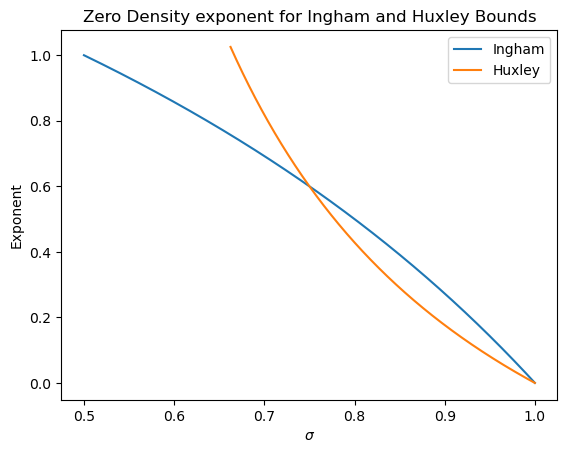
\includegraphics[width=\textwidth]{inghamhuxley1.png}
        \caption{The bounds for the exponent coincide at $\sigma=3/4$}
    \end{subfigure}
    \begin{subfigure}{0.4\textwidth}
        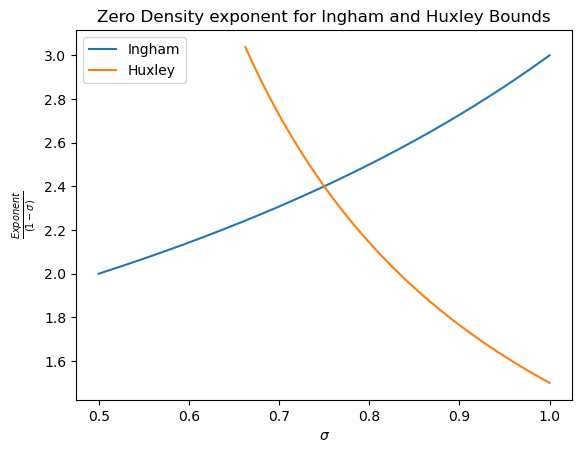
\includegraphics[width=\textwidth]{inghamhuxley2.png}
        \caption{$\sigma=3/4$ is also the bottleneck when written in Hoheisel's form.}
    \end{subfigure}

    \centering
    \begin{subfigure}{0.4\textwidth}
        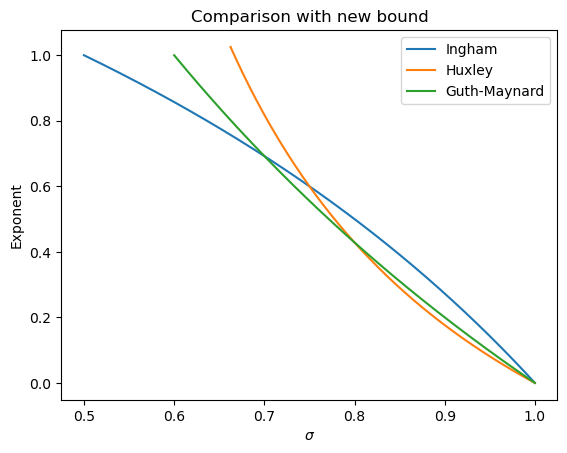
\includegraphics[width=\textwidth]{gm_1.png}
        \caption{Guth-Maynard's result improves in the range at $\sigma\in[7/10,8/10].$}
    \end{subfigure}
    \begin{subfigure}{0.4\textwidth}
        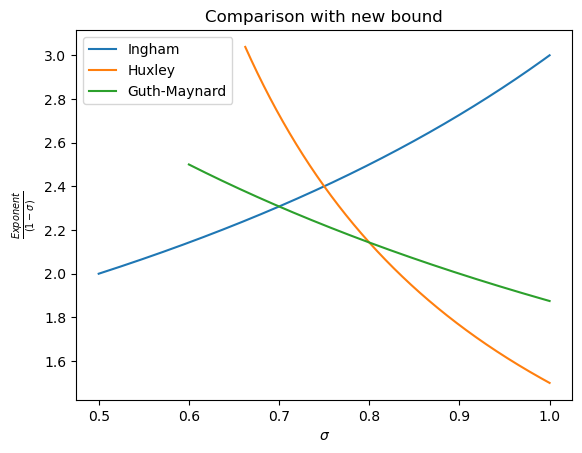
\includegraphics[width=\textwidth]{gm_2.png}
        \caption{The exponent is reduced around the bottleneck region.}
    \end{subfigure}
\end{figure}
	\section{Huxley's Proof of Zero Density}
\begin{theorem}[Huxley]
    We have  \[
    N(\sigma,t)\lesssim T^{\frac{12}{5}(1-\sigma)}.
    \]
\end{theorem}

Huxley's methodology for detecting zeros as follows. Let $M_x(s) \defeq \sum_{n=1}^{x} \mu(n)n^{-s}$. Since this also converges absolutely on $\Re(s)>1$, we can write the dirichlet series of $\zeta(s) M_x (s)$ as \[
    \zeta(s) M_x (s) \defeq \sum_{n}a_n n^{-s}
\]
for some choice of $a_n=a_n(x)$. The zeros of its analytic continuation will contain the zeros of $\zeta$. This may look inefficient as we may have introduced extra zeros from $M_x$, but the tradeoff is that we can bound these $a_n$'s.
\begin{proposition}
    We have  \[\begin{cases}
        a_1 = 1, & \\
        a_n = 0, & \textrm{if $1<n\leq x$},\\
        |a_n|\leq d(n), & \textrm{if $n>x$}.
    \end{cases}\]
\end{proposition}
\begin{proof}
    For all $n\leq x$, this follows from M\"obius inversion. For $n>x$, we just apply the trivial bound $|\mu(d)|\leq 1$ on \[
    a_n  = \sum_{d|n} \mu(d) .
    \]
\end{proof}

Let $y>x$ a parameter to be choosen later, and $y\leq T^A$ for an absolute constant $A$. We apply the Mellin transform to \begin{equation*}
    \begin{split}
    \sum_{n}a_n n^{-s} e^{-n/y}=&\frac{1}{2\pi i}\sum_{n}a_n n^{-s} \int_{2-i\infty}^{2+i\infty}\Gamma(w) y^w n^{-w} dw\\
    =&\frac{1}{2\pi i}\int_{2-i\infty}^{2+i\infty}\zeta(s+w)M_x(s+w)\Gamma(w) y^w dw.
    \end{split}
\end{equation*}
If we move the line of integration to $\Re(w) = 1/2 - \Re(s)$, we get simple pole residue contributions from $\zeta$ and $\Gamma$ \begin{equation}
    \label{huxleyperron}
    \begin{split}
    e^{-1/y}+\sum_{n>x}a_n n^{-s} e^{-n/y}=\sum_{n}a_n n^{-s} e^{-n/y}=&\zeta(s)M_x(s) +M_x(1)\Gamma(1-s)y^{1-s}\\+&
    \frac{1}{2\pi}\int_{-\infty}^{\infty}\zeta(\frac{1}{2}+i\Im(s)+iw)M_x(\frac{1}{2}+i\Im(s)+iw)\\ &\cdot \Gamma\left(\frac{1}{2}-\Re(s)+it\right) y^{\frac{1}{2}-\Re(s)+it} dt.
    \end{split}
\end{equation}
We take $y$ large enough so that $e^{-1/y}$ is close to $1$. Since $M_x(s)$ is an approximation of $1/\zeta$, we should expect that the term $\zeta(s)M_x(s)$ is about $1$ most of the time and the other terms are small. However, if $s$ is a zero of $\zeta$, then $\zeta(s)M_x(s)=0$, so at least one of the following things need to happen \begin{enumerate}[label=(\roman{*})]
    \item $|\sum_{n>x}a_n n^{-s} e^{-n/y}|$ is large.
    \item The integral in $t$ is large.
    \item $|M_x(1)\Gamma(1-s)y^{1-s}|$ is large.
\end{enumerate}
We thus transform the problem of detecting zeros to counting the number of occurences of extreme values. We will later see that type (iii) zeros are negligible, so we need to bound the number of type (i) and type (ii) zeros. 

\begin{lemma}
    Let $a$ be an arithmetic function, and $D_N(s)=\sum_{n\leq N}a(n)n^{s}.$
    If $W = \{t_j\}\subseteq [0,T]$ is a one-separated set such that \[
        |D_N(it_j)| > V \ \forall j,
    \]
    then \[
        |W|\ll \frac{\log^2 T}{V^\alpha} \int_{-(\log N)^{-1}}^{(\log N)^{-1}}
        \int_{0}^{T} |D_N(x+it)|^\alpha dt \ dx
        \]
    for $\alpha > 0$.
\end{lemma}
\begin{proof}
    With a cost of $O(1)$ we can consider $W\subseteq [(\log N)^{-1}, T-(\log N)^{-1}]$.
    Since $D_N$ is analytic, $|D_N|^\alpha$ is subharmonic. Let $B(t_j)$ describe a square-box of side length $(\log N)^-1$ centered at $it_j$ in the complex plane, then \begin{align*}
        V^\alpha \sum_{j} 1 \leq \sum_{j}|D(it_j)|^\alpha \leq \log^2 N \sum_{j} \int_{B(t_j)} |D(s)|^\alpha dA \leq \log^2 T \int_{-(\log N)^{-1}}^{(\log N)^{-1}}
        \int_{0}^{T} |D_N(x+it)|^\alpha dt \ dx.
    \end{align*}
\end{proof}

\begin{corollary}
   Let $W = \{t_j\}\subseteq [0,T]$ be a one-separated set such that \[
        \left|\zeta\left(\frac{1}{2}+it_j\right)\right|>V \ \forall j,
    \]
    then \[
    |W|\ll TV^{-4} \log^{O(1)}T.
    \]
\end{corollary}
\begin{proof}
    We have \[
        \left|\zeta\left(\frac{1}{2}+it\right)\right|\ll \sum_{n\leq \sqrt{T}}n^{-1/2-it},
    \]
    so applying the previous lemma on $D(s)=\sum_{n\leq \sqrt{T}}n^{-s}$ with $\alpha=4$ gives \begin{align*}
        |W|\ll \frac{\log ^2 T}{V^4} \int_{-2(\log T)^{-1}}^{2(\log T)^{-1}}
        \int_{0}^{T} |D_N(x+it)|^4 dt \ dx
    \end{align*}
\end{proof}

\begin{lemma}[Hal\'asz Inequality]
    \label{halasz}
    Let $a$ be an arithmetic function, and $D_N(s)=\sum_{n\leq N}a(n)n^{s}$, and $G=\sum_{n\leq N} |a(n)|^2.$
    If $W = \{t_j\}\subseteq [0,T]$ is a one-separated set such that \[
        |D_N(it_j)| > V \ \forall j,
    \]
    then 
    \[
        |W|\lesssim GNV^{-2} + G^3NTV^{-6}.
        \]
\end{lemma}
\begin{proof}
    Let $-\theta_j$ be the argument of $D(it_j)$, then we have \begin{align*}
        V|W|\leq \sum_j |D(it_j)| = \sum_j e^{\theta_j}D(it_j ) = \sum_{n\leq N} \sum_j e^{i\theta_j} a(n) n^{-it_j}.
    \end{align*}
    By Cauchy-Schwarz, this summation is \[
    \leq \left(\sum_{n\leq N} |a(n)|^2 \right)^{1/2}\left(\sum_{n\leq N} \bigg|\sum_j e^{i\theta_j} n^{-it_j}\bigg|^2 \right)^{1/2}.
    \]
    The first summation in this expression is $G$, so we want to bound the latter nested summation.
    Expanding the summation gives \begin{align*}
        \sum_{n\leq N} \bigg|\sum_j e^{i\theta_j} n^{-it_j}\bigg|^2 =& 
        \sum_{n\leq N} \sum_{j_1,j_2} e^{i\theta_{j_1}-i\theta_{j_2}} n^{it_{j_1}-it_{j_2}}\\
        \leq & |W|N + \sum_{j_1,j_2} \bigg|\sum_{n\leq N}  n^{it_{j_1}-it_{j_2}}\bigg|.
    \end{align*}
    \textcolor{red}{TODO}
\end{proof}

\begin{proof}[Proof of Huxley's Zero Density Theorem]
    From equation \ref{huxleyperron}, we take $y>6$ so that $e^{-1/y}>5/6$. We also truncate the sum in $n>x$ to $x<n\leq y^2$ with an error of $1/6$ for large enough $y$. Finally, we truncate the integral in $t$ to the range $|t|\leq B\log T$ with an error of $1/6$. Thus, $s$ is a zero only if \begin{enumerate}[label=(\roman{*})]
        \item $|\sum_{x<n\leq y^2}a_n n^{-s} e^{-n/y}|\geq \frac{1}{6}$, or
        \item $\frac{1}{2\pi}|\int_{-B\log T}^{B\log T}\zeta(\frac{1}{2}+i\Im(s)+iw)M_x(\frac{1}{2}+i\Im(s)+iw) \Gamma\left(\frac{1}{2}-\Re(s)+it\right) y^{\frac{1}{2}-\Re(s)+it} dt|\geq \frac{1}{6}$, or
        \item $|M_x(1)\Gamma(1-s)y^{1-s}|\geq \frac{1}{6}$ .
    \end{enumerate}
    Of the zeros $\rho = \beta+i\gamma$ of $\zeta$ in the region, at the cost of a factor of $\log T$, we take representatives such that if $\rho_1\neq \rho_2$ then $|\rho_1-\rho_2|\geq \textcolor{red}{1}$. 
    For Class (i) zeros, we split the sum dyadically to get \begin{equation}
    \label{class1dyadic}
    \bigg| \sum_{n\sim U, n\leq y^2} a(n)  n^{-\rho}e^{n/y}\bigg| \geq O((\log T)^{-1}),
    \end{equation}
    for some $x\leq U = 2^k\leq y$. Applying Lemma \ref{halasz}, we get that the number of times that equation \ref{class1dyadic} can happen for each $U$ is \[
    \lesssim U^{2-2\sigma} + U^{4-6\sigma}T\lesssim 
    \]
    (Note that the $\log$ factors are dominated by any choice of $T^\epsilon$)
\end{proof}

	\chapter{Guth-Maynard's Large Values Estimate near $\sigma = 3/4$}
	\section{Guth-Maynard's proof of Large Values of Dirichlet Polynomials}
In June 2024, Guth and Maynard published an improvement of the large values of Dirichlet polynomails estimate at $\sigma\in[7/10,8/10]$.
\begin{theorem}[Guth-Maynard Large Values Estimate]
    Let $(b_n)$ be a sequence of complex numbers such that $|b_n|\leq 1$ for all $n$, and $W=\{t_j\}_{j=1}^{|W|}$ be a $1$-separated set $\subseteq [0,T]$, such that \[
    \left|\sum_{n\sim N}b_n n^{it_j}\right|\geq V
    \]
    for each $t_j\in W$. Then \[
    |W|\lesssim N^2V^{-2}+N^{18/5}V^{-4}+TN{12/5}V^{-4}.
    \]
\end{theorem}
Let us compare this bound to Lemma \ref{halasz}, which states \[
|W|\lesssim N^2V^{-2}+TN^4V^{-6}.
\]
In the critical case $V=N^{3/4}, N\leq T^{5/6-\epsilon}$, the original bound will give \[
|W|\lesssim N^2N^{-3/2}+TN^4N^{-9/2}\lesssim N^{1/2}+ TN^{-1/2}\lesssim TN^{-1/2},
\]
while the bound by Guth and Maynard gives \[
|W|\lesssim N^2N^{-3/2}+N^{18/5}N^{-3}+TN^{12/5}N^{-3}\lesssim N^{1/2}+TN^{-3/5}\lesssim TN^{-3/5}.
\]
\subsection{Outline and Sketch of proof}
%\node[label=above/below/etc:{label}] (x) {}
The structure of the proof can be broken down as follows: We first notice that $|W|$ is bounded by the operator norm of a matrix $M$. This operator norm, using results from linear algebra, is bounded by the trace. Applying Poisson summation on the trace gives $4$ terms that are separately handled, which we will name $S_0$ to $S_3$. We will see that $S_0$ gives the `main term' that is consistent with the density hypothesis, $S_1$ is negligible, $S_2$ is bounded by a theorem by Heath-Brown, which we state below. 
\begin{theorem}[Heath-Brown]
    \label{heathbrown}
    Let $\mathcal{S}=\{(t_j,\chi_j)\}$ be one-separate, primitive characters of modulus $q$. Then 
    \[
        \sum_{\substack{(t_1,\chi_1)\\(t_2,\chi_2)}}\left|\sum_{n=1}^{N} b_n n^{-i(t_1-t2)}\chi_1\bar{\chi}_2(n)\right|^2 \lesssim  |\mathcal{S}|N^2+ |\mathcal{S}|^2N + |\mathcal{S}|^{5/4}(qT)^{1/2}N.
    \]
\end{theorem}
The most tricky term, $S_3$ is a summation over a three-dimensional lattice. We will see that $S_3$ is bounded by what is known as the \textit{additive energy} of the set $W$, defined by\[
    E(W)\defeq \#\{t_1,t_2,t_3,t_4\in W : |t_1+t_2-t_3-t_4|\ll T^\epsilon\}.
\]
This term describes the `additive structure' of $W$.
We see that $E(W)$ is bounded below by $|W|^2$, as the condition is satisfied when $t_1=t_3$ and $t_2=t_4$. Moreover, since $W$ is $1-separated$, the choice of $t_1,t_2,t_3$ fixes $O(1)$ choices for $t_4$, so $E(W)$ is bounded above by $|W|^3$. In the extreme case that the additive structure of $W$ is high, such as when $t_j=j\alpha$ for a constant $\alpha$, the energy of the set is $O(|W|^3)$. This definition naturally arrises from taking the fourth moment of the function \[
R(v)\defeq\sum_{t\in W} v^{it}.
\] 
This gives us \[
R(v)^4=\sum_{t_1,t_2,t_3,t_4\in W}v^{i(t_1+t_2-t_3-t_4)}.
\]

The naive choice $E(W)\leq W^3$ is slightly too loose to beat the Ingham-Huxley bound. However, an orthogonal bound can be found for $E(W)$ based on Heath-Brown's theorem. Finally, the bound in $7$ and $8$ combined is enough to give an improvement in most cases, a further refinement of the $S_3$ bound was required. This relies on the averaging over the affine summations of $R$.
 \[
        \sup_{0<M_1,M_2,M_3<M} \int\Bigg( \sum_{\substack{|m_1|\sim M_1\\|m_2|\sim M_2 \\ |m_3|\ll M_3}} \left|R\left(\frac{m_1 u+m_3}{m_2}\right)\right|\Bigg)^2 \ du \lesssim M^6 \|R\|_{L_2}^4+M^4\|f\|_{L_4}^4.
\] 

We give a quick sketch of the whole proof below. In the next section, we will give a full proof of the generalized statement of the theorem that considers primitive Dirichlet characters mod $q$. The proof of Guth-Maynard can be recovered by using the special case $q=1$.

\begin{figure} [t]
    \begin{tikzpicture}
        \begin{scope}[every node/.style={circle,thick,draw}]
            \node [label={[align=right]left:{$|W|$ is bounded by the operator\\ norm of a matrix $M$}}](A) at (0,0) {1};
            \node [label={[align=right]left:{$\|M\|^2$ is bounded by \\$\textrm{Tr}((M^*M)^k)^{1/k}$}}](B) at (0,-2) {2};
            \node [label={[align=right]left:{Poisson summation on $\textrm{Tr}((M^*M)^3)$,\\split in $4$ pieces}}](C) at (0,-4) {3};
            \node [label={[align=right] left:{$S_0$ gives main \\ term $N^2V^{-2}$}}](D) at (-6,-7) {4};
            \node [label={[align=right] left:{$S_1$ is negligible}}](E) at (-2,-7) {5};
            \node [label={[align=right] left:{$S_2$ reduces to\\ Heath-Brown}}](F) at (2,-7) {6};
            \node [label={[align=right] left:{$S_3$ is bounded\\ by Energy}}](G) at (6,-7) {7};
            \node [label={[align=right]left:{Energy bounded by \\ Heath-Brown}}](H) at (6,-10) {8};
            \node [label={[align=right]left:{Refinement of \\ $S_3$ bound}}](I) at (4,-8.5) {9};
        \end{scope}
        %\draw [dotted] (a) --  (b);
        \draw [->](A) -- (B);\draw [->](B) -- (C);
        \path [->](C) edge [bend left =13](D); \draw [->](C) -- (E); \draw [->](C) -- (F); \path [->](C) edge[bend left =20] (G);
        \draw[->] (G)--(H);\draw[->,red,dotted,thick] (G)--(I);\draw[dotted, red,->,thick] (I)--(H);
        %\draw (a) -- node[midway, below left]{1}(d) -- node[midway, below right]{2}(b);
        %\draw (a)-- node[midway, above left]{2} (c) --node[midway, above right]{1}(b);
\end{tikzpicture}
\caption{Graphical representation of Guth-Maynard proof outline}
\end{figure}
\subsubsection*{0. Setup}
First, as in the theorem, we let $(b_n)$ be a sequence of complex numbers such that $|b_n|\leq 1$ for all $n$, \[
D_n(t)\defeq \sum_{n\sim N}b_n n^{it},
\] $W=\{t_j\}_{j=1}^{|W|}$ be a $T^\epsilon$-separated set $\subseteq [0,T]$, such that \[
\left|D_n(t_j)\right|\geq V
\]
for each $t_j\in W$. Notice that we now let the set be $T^\epsilon$ separated for $\epsilon>0$. This means that we will give up a factor of $T^\epsilon$ in the final bound, but this makes many computations cleaner as this $T^\epsilon$ dominates the log factors. Moreover, we can introduce a bump function $\omega$ with support in $[1,2]$ to localize the summation, and rewrite \[
    D_n(t_j)=\sum_{n}\omega\left(\frac{n}{N}\right)b_n n^{it_j}.
\]
This is added for the Poisson summation in step $3$.
\subsubsection*{1. Bounding $|W|$ with operator norm}
We view $\vec{b}=(b_n)_{n\sim N}$ as a $N$-dimensional vector, and consider the $|W|\times N$ matrix, indexed by $j$ from $1$ to $|W|$ and $n\sim N$,\[
    M_{j,n}=n^{it_j}= \omega\left(\frac{n}{N}\right)n^{i t_j}.
\]
Then we can view the $j$-th entry of the product $M\vec{b}$ as $D_n(t_j)$. In other words \[
|M\vec{b}|^2\geq V^2{|W|}.
\]
However, we can bound $|M\vec{b}|$ using the operator norm of $M$ and $|b_n|\leq 1$ to get\[
    |M\vec{b}|^2\leq \|M\|^2|\vec{b}|^2 \leq \|M\|^2 N.
\]
Combined with the previous inequality, we get \begin{equation}
    \label{basicineq}
|W|\leq \|M\|^2 NV^{-2}.
\end{equation}

\subsubsection*{2. Bounding $\|M\|$}
An immediate way to proceed is to note that $\|M\|^2$ is the largest eigenvalue of $MM^*$, which in turn is bounded by sum of eigenvalues which is the trace of $M^*M$. However, this is somewhat inefficient. Consider $N$-dimensional vector that enumerates through the eigenvalues $(\lambda_n)$ of $MM^*$, so that the trace will be the $L_1$ norm of this vector. In principle, we would like the $L_{\infty}$ norm of this vector, so we can try to take $L_k$ norms of this vector for big $k$ to get close to $L_\infty$. Using an eigenbasis for $MM^*$, we can see that the $L_k$ norm is represented by \[
\left(\sum_{n\sim N}\lambda_n ^ {k}\right)^{1/k}= \textrm{Tr}((MM^*)^k)^{1/k}.
\]
We take $k=3$, which is the highest power we can afford given the tools at our disposal. This gives

\begin{equation}
    \label{traceineq}
    |W|\leq \textrm{Tr}((MM^*)^3)^{1/3} NV^{-2}.
\end{equation}

\subsubsection*{3. Expansion of $\rm{Tr}((MM^*)^3)$}
We first compute 

\begin{align*}
    (MM^*)_{n_1,n_2} = \sum_{t\in W} \omega\left(\frac{n_1}{N}\right)\omega\left(\frac{n_2}{N}\right)
    n_1^{-it_j}n_2^{it_j}
\end{align*}
so that\begin{align*}
    \textrm{tr}((M^*M)^3)=& \sum_{t_1,t_2,t_3\in W}\sum_{n_1,n_2,n_3\sim N} 
    \omega\left(\frac{n_1}{N}\right)^2\omega\left(\frac{n_2}{N}\right)^2\omega\left(\frac{n_3}{N}\right)^2 n_1^{i(t_1-t_3)}
   n_2^{i(t_2-t_1)}
    n_3^{i(t_3-t_2)}\\=& \sum_{t_1,t_2,t_3\in W}\sum_{n_1,n_2,n_3} 
    \omega\left(\frac{n_1}{N}\right)^2\omega\left(\frac{n_2}{N}\right)^2\omega\left(\frac{n_3}{N}\right)^2 \left(\frac{n_1}{N}\right)^{i(t_1-t_3)}
    \left(\frac{n_2}{N}\right)^{i(t_2-t_1)}
    \left(\frac{n_3}{N}\right)^{i(t_3-t_2)}.
\end{align*}
Let $h_t(u)\defeq \omega(u)^2 u^{it}$, we can apply Poisson summation in the inner integral over $n_1,n_2,n_3$ to get 
\begin{equation}\label{poissongm}
    \rm{tr}((M^*M)^3)= N^3\sum_{t_1,t_2,t_3\in W}\sum_{m_1,m_2,m_3}  \hat{h}_{t_1-t_3}(Nm_1)\hat{h}_{t_2-t_1}(Nm_2)\hat{h}_{t_3-t_2}(Nm_3).
\end{equation}
What we can gain here is that $\hat{h}_t{m}$ has decay in $t$ or $m$ based on the principle of non-stationary phase. 
\begin{lemma}[Non-stationary phase]
    We have for any integer $A>0$\begin{align*}
        |\hat{h}_t(\xi)|\ll_A \frac{1+|t|^A}{|\xi|^A},\\
        |\hat{h}_t(\xi)|\ll_A \frac{1+|xi|^A}{|t|^A}. 
    \end{align*}
\end{lemma}
\begin{proof}
   We have \[
   \hat{h}_t(\xi)=\int \omega(u)^2u^{it}e^{2\pi i \xi u} du.\]
   By repeated integration by parts on $\omega(u)^2u^{it}$ and $e^{2\pi i \xi u}$, we get \[
    |\hat{h}_t(\xi)|=\left|\int (2\pi i \xi)^{-A} e^{2\pi i \xi u}  \frac{d^A}{(du)^A}\left(\omega^2(u)u^{it}\right) du\right| \ll_A \frac{1+|t|^A}{|\xi|^A}.
   \]
   A similar argument for integration by parts on $\omega(u)^2e^{2\pi i \xi u}$ and $u^{it}$ gives \[
    |\hat{h}_t(\xi)|=\left|\int \frac{1}{(it+1)(it+2)\ldots(it+A)}u^{it+A}  \frac{d^A}{(du)^A}\left(\omega^2(u)e^{2\pi i \xi u}\right) du \right|\ll_A \frac{1+|\xi|^A}{|t|^A}.
   \]
\end{proof}
This means that we can handle terms in equation \ref{poissongm} if $m_i$ is small and $t_j-t_k$ is big, or  $m_i$ is big and $t_j-t_k$ is small. With this in mind, we split the sum over $n_1,n_2,n_3$ in the equation into four parts. $S_0$, where all three $m$ terms are zero, $S_1$, where exactly one of the $m$ terms is non-zero, $S_2$, where exactly two of the $m$ terms are non-zero, and $S_3$, where all three $m$ terms are non-zero.
That is,

\[\rm{tr}((M^*M)^3)= S_0+S_1+S_2+S_3, \]
where \[
S_j = N^3\sum_{m_1,m_2,m_3, \#\{m_k=0\}=j} I_m,
\]
\[
I_m=I_{(m_1,m_2,m_3)}\defeq N^3\sum_{t_1,t_2,t_3\in W}\hat{h}_{t_1-t_3}(Nm_1)\hat{h}_{t_2-t_1}(Nm_2)\hat{h}_{t_3-t_2}(Nm_3).
\]

\subsubsection*{4. Bounding $S_0$}
$S_0$ only has one term in the sum. \[
S_0 = N^3\sum_{t_1,t_2,t_3\in W} \hat{h}_{t_1-t_3}(0)\hat{h}_{t_2-t_1}(0)\hat{h}_{t_3-t_2}(0)
\]
Now we can apply that $W$ is $T^\epsilon$ separated, so there is a trivial bound $|W|\leq T$ and $\hat{h}_{t_j-t_k}$ is negligible by the principle of non-stationary phase. So we can only consider \[
S_0 = N^3\sum_{t\in W}\hat{h}_0(0) + O(T^{-100}) = N^3|W|\|\omega\|_{L_2}^6.
\]Taking the cube root, this term gives $O(N^2V^{-2}|W|)$ in equation \ref{traceineq}. This is strikingly similar to the $N^2V^{-2}$ term that the density hypothesis conjectures. Guth and Maynard isolates this term by introducing the following lemma.
\begin{lemma}\label{gmtrace}
    Let $A$ be an $m\times n$ matrix. Then 
    \[\|A\| \leq 2\left(\rm{tr}((AA^*)^3)-\frac{\rm{tr}(AA^*)^3}{m^2}\right)^{1/6}+2\left(\frac{\rm{tr}(AA^*)}{m}\right)^{1/2}.
    \]
\end{lemma}
\begin{proof}
    This is Lemma 4.2 from Guth-Maynard. \cite{}
\end{proof}
Applying this lemma, we can compute that \[
    \rm{tr}(MM^*) =\sum_{n\sim N} \sum_{t\in W} \omega\left(\frac{n}{N}\right)^2 n^{-t} n^{t}= |W|\sum_n \omega\left(\frac{n}{N}\right)^2.
\]
Applying Poisson summation, this equals \[
    |W|\sum_m N \hat{h}_0(mN).
\]
By non-stationary phase use the rapid decay of $\hat{h}_0(\xi)$ in $\xi$ to only consider the term $m=0$ at the cost of $N^{-100}$.
Therefore, $\rm{tr}(MM^*)=|W|N\|\omega\|_{L_2}^2+O(N^{-100})$.
Lemma \ref{gmtrace} gives \[
|W|\ll NV^{-2}(N+(S_0+S_1+S_2+S_3-N^3|\omega|_{L_2}^6|W|)^{1/3}) \ll N^2V^{-2}+  NV^{-2}(S_1+S_2+S_3)^{1/3}. 
\]


\subsubsection*{5. Bounding $S_1$}
By symmetry in $m_1,m_2,m_3$, we can consider the terms where $m_3\neq 0$ at a cost of a factor of $3$.
Then \[
S_1 =3 N^3\sum_{m\neq 0} \sum_{t_1,t_2,t_3\in W}\hat{h}_{t_1-t_3}(0)\hat{h}_{t_2-t_1}(0)\hat{h}_{t_3-t_2}(mN).
\] 
This term is bounded by non-stationary phase. If $|m|>T^{1+\epsilon}/N$, then $|m|/|t_3-t_2|< T^\epsilon$, so we can truncate the sum to $|m|\leq T^{1+\epsilon}/N$ with an error of $O_\epsilon(T^{-100})$. In this range, if $t_1\neq t_3$ or $t_2\neq t_1$, then they are $T^\epsilon$ apart, then we get rapid decay in $\hat{h}_{t_1-t_3}(0)$ or $\hat{h}_{t_2-t_1}(0)$ to be $O_\epsilon{T^{-100}}$. But when $t_1=t_2=t_3$, we get decay in the last term $\hat{h}_0(mN)$. Combining all cases, this term is negligible.

\subsubsection*{6. Bounding $S_2$}

By symmetry again we can consider the terms where $m_1,m_2\neq 0,m_3=0$.Then \begin{align*}
    S_2=&3 N^3\sum_{m_1,m_2\neq 0} \sum_{t_1,t_2,t_3\in W}\hat{h}_{t_1-t_3}(m_1N)\hat{h}_{t_2-t_1}(m_2N)\hat{h}_{t_3-t_2}(0).
\end{align*}
Due to decay of the last term in $|t_3-t_2|$, we can only consider the terms $t_3=t_2$ with error $O_{\epsilon,A}(T^{-A})$. Then we can rewrite
\begin{align*}
    3 N^3\hat{h}_{0}(0)\sum_{m_1,m_2\neq 0} \sum_{t_1,t_2\in W}\hat{h}_{t_1-t_2}(m_1N)\hat{h}_{t_2-t_1}(m_2N) &= 3 N^3\hat{h}_{0}(0)\sum_{m_1,m_2\neq 0} \sum_{t_1,t_2\in W}\hat{h}_{t_1-t_2}(m_1N)\hat{h}_{t_1-t_2}(-m_2N)\\
    &= 3 N^3\hat{h}_{0}(0)\sum_{t_1,t_2\in W}\left(\sum_{m\neq 0}\hat{h}_{t_1-t_2}(mN)\right)^2.
\end{align*}
Poisson summation gives \[
N \sum_m \hat{h}_{t_1-t_2}(mN) = \sum_n h_{t_1-t_2}\Big(\frac{n}{N}\Big)=\sum_{n} \omega\left(\frac{n}{N}\right) n^{i(t_1-t_2)}.
\]
\begin{remark}
    Here we have added in the terms for $m=0$. This is somewhat lossy for terms $t_1=t_2$. However, a variation of the argument (and applying Heath-Brown's result in the end) gives a tighter bound, which will be adapted for the general proof.
\end{remark}

\subsubsection*{7. Bounding $S_3$}
$S_3$ sums over most points on the $3$-dimensional lattice. By symmetry, we can consider only the terms with $m_1\leq m_2\leq m_3$ with an error factor of $6$.
Recall that \[
I_m=N^3\sum_{t_1,t_2,t_3\in W}\hat{h}_{t_1-t_3}(Nm_1)\hat{h}_{t_2-t_1}(Nm_2)\hat{h}_{t_3-t_2}(Nm_3).
\]
By the the principle of non-stationary phase, we can truncate the sum across $I_m$ to $|m_1|,|m_2|,|m_3|\lesssim T/N$, at the cost of $O\epsilon(T^{-100})$, as $t_j-t_k=O(T)$.
We expand $\hat{h}$ in integral form, so that \begin{align*}
    I_{\vec{m}}&=N^3\sum_{t_1,t_2,t_3\in W}\int_{\reals^3} \omega(u_1)^2\omega(u_2)^2\omega(u_3)^2 u_1^{i(t_1-t_3)}u_2^{i(t_2-t_1)}u_3^{i(t_3-t_2)} e(-N\vec{m}\cdot \vec{u}) d\vec{u}\\ &=N^3\sum_{t_1,t_2,t_3\in W}\int_{\reals^3} \tilde{\omega}(\vec{u}) \Big(\frac{u_1}{u_2}\Big)^{it_1}\Big(\frac{u_2}{u_3}\Big)^{it_2}\Big(\frac{u_3}{u_1}\Big)^{it_3}e(-N\vec{m}\cdot \vec{u}) d\vec{u}
\end{align*}
For $\tilde{\omega}(\vec{u})=\omega(u_1)^2\omega(u_2)^2\omega(u_3)^2$. Because $\tilde{\omega}$ is supported away from $u_3=0$, we can introduce the change of variables $v_1=u_1/u_3$, $v_2=u_2/u_3$. The Jacobian is $u_3^2$, and $u_1/u_2=v_1/v_2$, so that \begin{align*}
    I_{\vec{m}}& = N^3\sum_{t_1,t_2,t_3\in W}\int_{\reals^3} u_3^2 \tilde{\omega}(v_1u_3,v_2u_3,u_3) \Big(\frac{v_1}{v_2}\Big)^{it_1} v_2^{it_2}\Big(\frac{1}{v_1}\Big)^{it_3}e(-Nu_3(m_1v_1+m_2v_2+m_3)) dv_1\ dv_2 \ du_3\\ 
    & = N^3\sum_{t_1,t_2,t_3\in W}\int_{\reals^2}\int_{\reals} u_3^2 \tilde{\omega}(v_1u_3,v_2u_3,u_3)e(-Nu_3(m_1v_1+m_2v_2+m_3))   du_3 \  \Big(\frac{v_1}{v_2}\Big)^{it_1} v_2^{it_2}\Big(\frac{1}{v_1}\Big)^{it_3}  dv_1\ dv_2 
\end{align*}
The inner integral in $u_3$ places restrictions on the domain of integration. First, the support of $\tilde{\omega}$ is $[1,2]\times [1,2]\times [1,2]$. Thus, if it is non-zero, we have $v_1u_3,v_2u_3,u_3\in [1,2]\implies v_1,v_2\in [1/2,2]$. Therefore, we can restrict the outer integral in $v_1$ and $v_2$ to this range. Next, since $v_1,v_2=O(1)$, the chain rule gives\[
\left(\frac{\partial}{\partial u_3}\right)^j{\omega}(v_1u_3,v_2u_3,u_3)\ll_j 1.\]
Therefore, we can apply the repeated integration by parts to get rapid decay of the integral in $|N(m_1v_1+m_2v_2+m_3)|$. In particular, we can truncate the integral to the range $|N(m_1v_1+m_2v_2+m_3)|\ll T^\epsilon$ at an error of $O_{\epsilon}(T^{-100})$, and use \[
    \int_{\reals} u_3^2 \tilde{\omega}(v_1u_3,v_2u_3,u_3)e(-Nu_3(m_1v_1+m_2v_2+m_3))   du_3=O(1)
\]
in this range by the compact support of $\tilde{\omega}$. This gives us \begin{equation}
    |I_{\vec{m}}|\leq \Bigg|N^3 \sum_{t_1,t_2,t_3\in W}\int\displaylimits_{\substack{
        |v_1m_1+v_2m_2+m_3|\lesssim \frac{1}{N}\\
        \frac{1}{2}\leq v_1,v_2\leq 2
    }} \Big(\frac{v_1}{v_2}\Big)^{it_1} v_2^{it_2}\Big(\frac{1}{v_1}\Big)^{it_3}  dv_1\ dv_2 \Bigg|+O_{\epsilon}(T^{-100}).
\end{equation}
Recall that in the outline we defined\[
R(v)\defeq\sum_{t\in W} v^{it}.
\]
Exchanging the summation and integral, we get the term \begin{align*}
    &\Bigg| N^3 \int\displaylimits_{\substack{
        |v_1m_1+v_2m_2+m_3|\lesssim \frac{1}{N}\\
        \frac{1}{2}\leq v_1,v_2\leq 2
    }} R\Big(\frac{v_1}{v_2}\Big) R({v_2}\Big) R\Big(\frac{1}{v_1}\Big) dv_1\ dv_2 \Bigg|\\
    \leq & N^3 \int\displaylimits_{\substack{
        |v_1m_1+v_2m_2+m_3|\lesssim \frac{1}{N}\\
        \frac{1}{2}\leq v_1,v_2\leq 2
    }} \Bigg|R\Big(\frac{v_1}{v_2}\Big) R({v_2}\Big) R\Big(\frac{1}{v_1}\Big)\Bigg| dv_1\ dv_2 \\
    =  & N^3 \int\displaylimits_{\substack{
        |v_1m_1+v_2m_2+m_3|\lesssim \frac{1}{N}\\
        \frac{1}{2}\leq v_1,v_2\leq 2
    }} \Bigg|R\Big(\frac{v_2}{v_1}\Big) R({v_2}\Big) R({v_1})\Bigg| dv_1\ dv_2,
\end{align*}
where the last step, we used \[
|R(v^{-1})| = \Big|\sum_{t\in W} v^{-it}\Big| = \Big|\sum_{t\in W} v^{it}\Big| = |R(v)|.
\]
Now we fix $v_1$, and consider the integral in $v_2$ in the range \[
    |v_1m_1+v_2m_2+m_3|\lesssim \frac{1}{N} \implies \Big|v_2 -\frac{v_1m_1+m_3}{-m_2}\Big|\lesssim \frac{1}{|m_2| N}.
\]
If we enforce the conditions $|m_1|\leq |m_2|\leq|m_3|$ and $v_2\asymp 1$, we see that the domain of integration is empty unless $|m_2|\asymp |m_3|$. Thus, we can break the sum across \[\sum_{|m_1|,|m_2|,|m_3|\lesssim T/N}\] to be \[\log T^{1+\epsilon}/N \ \rm{sup}_{U=2^j, V\leq U} \sum_{\substack{|m_1|\sim V\\  |m_2|, |m_3|\sim U}}.\]
Moreover, we integrate in $v_2$ over a very small neighborhood of width $\lesssim 1/N$ around $v_2=({v_1m_1+m_3})/({-m_2})$. In principle, we can estimate this integral by taking the value of $R$ at this point to get \[
    \approx  \frac{N}{|m_2|} \int\displaylimits_{\substack{
        \frac{1}{2}\leq v_1\leq 2
    }} \Bigg|R\Big(\frac{v_1m_1+m_3}{-v_1m_2}\Big) R(\frac{v_1m_1+m_3}{-m_2}\Big) R({v_1})\Bigg| dv_1.
\]
This is made precise by apply to a $(1/N|m_2|)$-smoothened version of $R$, stated in Proposition \ref{dyadics_3}. Finally, H\"older's inequality gives a bound of \begin{align*}
    \Big\|R\Big(\frac{vm_1+m_3}{-vm_2}\Big) \Big\|_{\substack{L_4\\ v\asymp 1}}\Big\|R\Big(\frac{vm_1+m_3}{-m_2}\Big) \Big\|_{\substack{L_4\\ v_1\asymp 1}}\Big\|R(v) \Big\|_{\substack{L_2\\ v_1\asymp 1}}
\end{align*}

The second moment of $R$ is bounded by the size of $W$. Indeed, we have \begin{align*}
    \int_{v\asymp 1} |R(v)|^2 dv =  \sum_{t_1,t_2\in W} \int_{v\asymp 1} R(v)^{i(t_1-t_2)} dv.  
\end{align*}
If $t_1-t_2\neq 0$, then $|t_1-t_2|>T^\epsilon$, so the oscillatory integral will be negligible by the fast decay. There are $|W|$ terms satisfying $t_1=t_2$, and each contributes $O(1)$ to the sum. Similarly, the fourth moment of $R$ is bounded by the energy, recalling its definition \[
    E(W)\defeq \#\{t_1,t_2,t_3,t_4\in W : |t_1+t_2-t_3-t_4|\ll T^\epsilon\}.
\]
We get
\begin{align*}
    \int_{v\asymp 1} |R(v)|^2 dv =   \sum_{t_1,t_2,t_3,t_4\in W} \int_{v\asymp 1}  R(v)^{i(t_1+t_2-t_3-t_4)} dv, 
\end{align*}
and the terms in the summation are negligble unless $|t_1+t_2-t_3-t_4|\ll T^\epsilon$. Assembling everything together gives an initial bound of \[
S_3\lesssim T^2E(W)^{1/2}|W|^{1/2}.
\]


\subsubsection*{9. Refinement of $S_3$ bound}

Recall that in the previous section, we summed across 
\[
    \sum_{\substack{|m_1|\sim V\\ |m_2|, |m_3|\sim U}} \frac{N}{|m_2|} \int\displaylimits_{\substack{
        \frac{1}{2}\leq v_1\leq 2
    }} \Bigg|R\Big(\frac{v_1m_1+m_3}{-v_1m_2}\Big) R\Big(\frac{v_1m_1+m_3}{-m_2}\Big) R({v_1})\Bigg| dv_1
\]
By repeatedly applying Cauchy-Schwartz, we can move the summation into the integral and obtain terms that resembles the form \[
   \int_{v_1\asymp 1} \sum_{\substack{|m_1|\sim V\\ |m_2|, |m_3|\sim U}}  \Big| R\Big(\frac{v_1m_1+m_3}{-m_2}\Big)\Big|^2 dv_1.
\]
The term $(v_1m_1+m_3)/(-m_2)$ describes an affine transformation in $v_1$. Therefore, averaging over all the affine transformations, we may expect that this estimates some $L^k$ norm of $R$. Indeed, we have Lemma \ref{affinetrans} that gives us this estimate. This improves the bound on $S_3$ to\[
S_3\lesssim T^2|W|^{3/2}+TN|W|^{1/2}E(W)^{1/2}.
\]
This gives an improvement from the previous bound for the case $N \ll T^{1-\delta_1}$ and $E(W)\gg |W|^{3-\delta_2}$ for some small $\delta$'s.


\subsubsection*{8. Bound on $E(W)$}
Finally, we give an orthogonal bound on the energy of the set $W$. The is that if $|t_1+t_2-t_3-t_4|$ is small, then we can approximate \[
D_N(t_4) \approx D_N(t_1+t_2-t_3).
\]
This is made precise by applying a smoothing of $D_N$ over a width of $\lesssim 1$.
Therefore, since the choice of $t_4$ is fixed by the choice of $t_1,t_2,t_3$, we have\[
E(W)V^2\leq \sum_{|t_1-t_2-t_3-t_4|\lesssim 1} |D_N(t_4)|^2 \approx \sum_{|t_1-t_2-t_3-t_4|\lesssim 1} |D_N(t_1+t_2-t_3)|^2 \leq \sum_{t_1,t_2,t_3\in W} |D_N(t_1+t_2-t_3)|^2.
\]
Now we can expand $|D_N(t_1+t_2-t_3)|^2$ to get \begin{align*}
    \sum_{t_1,t_2,t_3\in W} |D_N(t_1+t_2-t_3)|^2=& \sum_{t_1,t_2,t_3\in W}\sum_{n_1,n_2\sim N} b_{n_1} \bar{b}_{n_2} \Big(\frac{n_1}{n_2}\Big)^{i(t_1+t_2-t_3)}\\ 
    =&\sum_{n_1,n_2\sim N} b_{n_1} \bar{b}_{n_2}\sum_{t_1,t_2,t_3\in W}\Big(\frac{n_1}{n_2}\Big)^{i(t_1+t_2-t_3)}\\ 
    \leq& \sum_{n_1,n_2\sim N} \Big|R\Big(\frac{n_1}{n_2}\Big)R\Big(\frac{n_1}{n_2}\Big)R\Big(\frac{n_2}{n_1}\Big)\Big|\\ 
    \leq& \sum_{n_1,n_2\sim N} \Big|R\Big(\frac{n_1}{n_2}\Big)\Big|^3.
\end{align*}
Now we can apply the trivial bound $|R|\leq |W|$ to get that \[
    E(W)\lesssim V^{-2}|W|\sum_{n_1,n_2\sim N} \Big|R\Big(\frac{n_1}{n_2}\Big)\Big|^2.
\]
This is in turn bounded by Heath-Brown's result as \begin{align*}
    \sum_{n_1,n_2\sim N} \Big|R\Big(\frac{n_1}{n_2}\Big)\Big|^2 &=
    \sum_{n_1,n_2\sim N}\sum_{t_1,t_2\in W} \Big(\frac{n_1}{n_2}\Big)^{i(t_1-t_2)}\\ 
    &= \sum_{t_1,t_2\in W} \Big|\sum_{n\sim N} n^{i(t_1-t_2)} \Big|^2.
\end{align*}
This is enough to give an improvement on Ingham-Huxley's result, but can be further improved using Cauchy Schwartz on the third moment \begin{align*}
    \sum_{n_1,n_2\sim N} \Big|R\Big(\frac{n_1}{n_2}\Big)\Big|^3 \leq 
    \Bigg(\sum_{n_1,n_2\sim N} \Big|R\Big(\frac{n_1}{n_2}\Big)\Big|^2 \Bigg)^{1/2} \Bigg(\sum_{n_1,n_2\sim N} \Big|R\Big(\frac{n_1}{n_2}\Big)\Big|^4\Bigg)^{1/2}.
\end{align*}
The fourth moment can be reduced back to the second moment by taking representative classes of $\lfloor t_1-t_2 \rfloor$, thus can also be bounded using Heath-Brown's result.
	
	 \chapter{Towards a Hybrid Zero Density Result}

\iffalse

\textit{Here I will document some progress with working with
the hybrid version of Guth-Maynard. This section will be removed when I send the draft to Prof. Wunsch.}
\fi
We would like to generalize Guth and Maynard's result to $L$-functions. Specifically, let $\chi$ be a \hyperref[dcharacter]{Dirichlet character}. we are interested in the the zeros of the function defined by \[
L(s,\chi)\defeq\sum_{n} \frac{\chi(n)}{n^{-s}}
\]
on $\Re(s)>1$ and its analytic continuation on the whole complex plane. The zeta function is a special case of an $L$-function with the Dirichlet character $1$ everywhere. The structure of the arguments for analytic continuation of an $L$-function, its line of symmetry along $\Re(s) = 1/2$, and the locations of zeros are very similar to that of the zeta function. This motivates the Generalized Riemann Hypothesis. \begin{conjecture} [Generalized Riemann Hypothesis]
    The \text{Generalized Riemann Hypothesis} asserts that on the critical strip, \[
    L(s,\chi)=0 \implies \Re(s)=\frac{1}{2},
    \]
    for any Dirichlet character.
\end{conjecture}
The Generalized Riemann Hypothesis leads to even stronger for primes in short intervals. Namely, fix an integer $q$, we have that \[
\sum_{\substack{n\leq N\\ n\equiv a\mod q}}\Lambda(n) = \begin{cases}
    \frac{1}{\phi(q)} N + O(x^{2+o(1)}), & \textrm{if $\gcd(a,q)=1$}\\
    o(n),& \textrm{otherwise.}
\end{cases}
\]
This means that not only that the Prime Number Theorem holds in intervals of $x^{2+\epsilon}$, the distribution of primes in each of the residual classes (coprime to $q$) are uniform at this scale too. Noticing that we can modify Huxley's proof with \[
M_{x,\chi} = \sum_{n\leq x} \chi(n) \mu(n) n^{-s},
\]
we have \[
L(s,\chi)M_{x,\chi} = \sum_{n} a_n \chi(n) \mu(n) n^{-s}.
\]

Thus, we can reproduce a similar proof on the zero density of $L$-functions. 
\begin{definition}[Zero Density for $L$-functions]
    Let $N(\sigma,\chi,T)$ denote the number of zeros of the $L$-function $L(-,\chi)$ with real part greater than $\sigma$ and imaginary part between $-T$ and $-T$. That is \[
    N(\sigma,\chi,T) \defeq \#\{\rho=\beta+i\gamma \ | \ \beta\geq \sigma, |\gamma|\leq T\}.
    \]
    For backwards compatibility with our previous definition, we take $N(\sigma,T)\defeq N(\sigma, 1,T)$.
\end{definition}
The hybrid analogs of the zero density bounds of Ingham and Huxley are known.
\begin{theorem}[Hybrid Ingham bound for zero density]
    Let $1/2\leq \sigma\leq 3/4$. We have \[
        \sum_{\chi^* }N(\sigma,\chi^*,t)\lesssim (qT)^{\frac{3(1-\sigma)}{2-\sigma}},
        \]
        where $\sum_{\chi^*}$ sums over all the primitive characters $\chi^*$ of modulus $q$.
\end{theorem}
\begin{theorem}[Hybrid Huxley bound for zero density]
    Let $3/4\leq \sigma\leq 1$. We have \[
        \sum_{\chi^* }N(\sigma,\chi^*,t)\lesssim (qT)^{\frac{3(1-\sigma)}{3\sigma-1}},
        \]        
        where $\sum_{\chi^*}$ sums over all the primitive characters $\chi^*$ of modulus $q$.
\end{theorem}

The method for detecting zeros is very similar to Huxley's proof above with the slight change in definition of $M_{x,\chi}$. This argument then reduces to bounding the number of times large values of Dirichlet polynomials can occur. Therefore we want a result in the form:
\begin{quotation}  
Let $W=\{(t_j,\chi_j)\}$ be a set such that each $\chi_j$ is a primitive Dirichlet character of modulus $q$, and $|t_j-t_k|\geq 1$ if $j\neq k$ and $\chi_j=\chi_k$. (That is, the $t$'s are $1$-separated if the characters are the same.)Let $|b_n|\leq 1$ be a sequence of numbers indexed in $n$, and suppose also that \[
\Bigg|\sum_{n\sim N} b_n\chi_j(n)n^{it_j} \Bigg|>V.
\]
We want to find a bound on $|W|$.
\end{quotation}
\section{Statement of Main Theorem}
Our result is as follows: 
\begin{theorem}\label{mainthm}
    Let $W=\{(t_j,\chi_j)\}$ be a set such that each $\chi_j$ is a primitive Dirichlet character of modulus $q$, and $t_j\in[0,T]$. Further assume that $|t_j-t_k|\geq T^\epsilon$ if $j\neq k$ and $\chi_j=\chi_k$. Let $|b_n|\leq 1$ be a sequence of numbers indexed in $n$, $\omega$ be a smooth bump function that equals $1$ on $[6/5,9/5]$ and has support in $[1,2]$ (thus $\omega^{(A)}\ll_A 1$ for all $A$). Let $V=N^{\sigma}$, where $[7/10,8/10]$, and $N=(qT)^{5/6}$. Suppose also that \[
    |D_N(t_j,\chi_j)|\defeq\Bigg|\sum_{n\sim N} \omega\Bigg(\frac{n}{N}\Bigg)b_n\chi_j(n)n^{it_j} \Bigg|>V.
\]
for all $(t_j,\chi_j)\in W$.
Then \[
|W|\ll (qT)N^{(12-20\sigma)/5+o_{\epsilon}(1)}
\]
for \textbf{almost all} values of $q$ that satisfy $\omega(q)= O(\log\log q)$ by the Erd\"os-Kac Theorem.
\end{theorem}

The idea of the proof is similar to Guth and Maynard's proof. We can define a $|W|\times N$ matrix $M$ with entries
\[
    M_{t_j,\chi_j,n} = \chi_j(n)n^{it_j}
\]
for $(t_j,\chi_j)\in W$ and $n\sim N$, and bound its operator norm in the exact same way: taking it to the $M^*M$ to the third power and calculating its trace. We will highlight similar ideas when they come up.

\section{The matrix $M$ and its trace expansion}
We define $M$ a $|W |\times N$ matrix with entries
\[
    M_{(t_j,\chi_j),n} = \omega\Big(\frac{n}{N}\Big)\chi_j(n)n^{it_j}
\]
for $(t_j,\chi_j)\in W$ and $n\sim N$.
Thus by the same reasoning that $(M\vec{b})_j=D_N(t_j,\chi_j)$,
we want to bound the size of $W$ by trace of the matrix \[
\textrm{tr}((M^*M)^3).
\].
\begin{proposition} \label{Tracebound}
    Let \[
    P(n,(t_1,\chi_1),(t_2,\chi_2))\defeq \omega\left(\frac{n}{N}\right)^2 \left(\frac{n}{N}\right)^{i(t_2-t_1)}\chi_2\bar{\chi}_1(n),
    \]
    and \[
    S \defeq \sum_{\substack{(t_1,\chi_1),(t_2,\chi_2),\\(t_3,\chi_3)\in W\\ (*)} }\ \sum_{n_1,n_2,n_3\sim N} 
    P(n_1,(t_1,\chi_1),(t_3,\chi_3))P(n_2,(t_2,\chi_2),(t_1,\chi_1))P(n_3,(t_3,\chi_3),(t_2,\chi_2)),
    \]
    where the condition $(*)$ denotes that the three pairs are not all identical.
    We have 
    \[
        |W|\ll N^2 V^{-2} + N V^{-2} S^{1/3}.
    \]
    
\end{proposition}


\begin{lemma}\label{trace formula}
    We have 
    \[
        |W|\ll N V^{-2}\left(\frac{\rm{tr}(AA^*)}{|W|}\right) + N V^{-2}\left(\rm{tr}((MM^*)^3)-\frac{\rm{tr}(MM^*)^3}{|W|^2}\right)^{1/3}.
    \]
\end{lemma}


\begin{lemma}\label{hilberttrace}
    Let $A$ be an $m\times n$ matrix. Then 
    \[\|A\| \leq 2\left(\rm{tr}((AA^*)^3)-\frac{\rm{tr}(AA^*)^3}{m^2}\right)^{1/6}+2\left(\frac{\rm{tr}(AA^*)}{m}\right)^{1/2}.
    \]
\end{lemma}
\begin{proof}
    This is Lemma 4.2 from Guth-Maynard. \cite{GM2024}
\end{proof}


\begin{proof}[Proof of Proposition \ref{trace formula}]
    Consider the product $M\vec{b}$. The $j$-th entry is exactly $D_n(t_j,\chi_j)$. Thus we have \[
    V^2|W|\leq |M \vec{b}|^2 \leq \|M\|^2|\vec{b}|^2\leq \|M\|^2N.
    \]
    Applying lemma \label{hilberttrace} gives the desired result.
\end{proof}


We now compute the expression for the traces.
\begin{lemma}[Explicit Expression of Traces]
    Let \[
    P(n,(t_1,\chi_1),(t_2,\chi_2))\defeq \omega\left(\frac{n}{N}\right)^2 \left(\frac{n}{N}\right)^{i(t_2-t_1)}\chi_2\bar{\chi}_1(n).
    \]
    We have 
    \begin{align*}
        \rm{tr}(M^*M) = & \ |W|\sum_{n\sim N, \gcd (n,q)=1} \omega\left(\frac{n}{N}\right)^2, \\
        \rm{tr}((M^*M)^3)=&\sum_{\substack{(t_1,\chi_1),(t_2,\chi_2),\\(t_3,\chi_3)\in W}}\sum_{n_1,n_2,n_3\sim N} 
        P(n_1,(t_1,\chi_1),(t_3,\chi_3))P(n_2,(t_2,\chi_2),(t_1,\chi_1))P(n_3,(t_3,\chi_3),(t_2,\chi_2)).
    \end{align*}
\end{lemma}
\begin{proof}
   % We compute the traces of $MM^*$ and $(MM^*)^3$ instead, as this makes the calculations cleaner.
    We see that \begin{align*}
        (MM^*)_{(t_j,\chi_j),(t_k,\chi_k)} = \sum_{n\sim N} \omega\left(\frac{n}{N}\right)^2 n^{i(t_k-t_j)}\bar{\chi}_j\chi_k(n) = \sum_{n\sim N}P(n,(t_k,\chi_k),(t_j,\chi_j))N^{i(t_k-t_j)},
    \end{align*}
    so that \begin{align*}
        \textrm{tr}(MM^*) =& \sum_{(t_j,\chi_j)} \sum_{n\sim N} P(n,(t_j,\chi_j),(t_j,\chi_j)) \\
        =&|W|\sum_{n\sim N} |\chi_j(n)|\omega\left(\frac{n}{N}\right)^2.
    \end{align*}
    For the third power, we have 
    \begin{align*}
        (MM^*)^3_{(t_j,\chi_j),(t_k,\chi_k)} = \sum_{(t_1,\chi_1),(t_2,\chi_2)\in W}   (MM^*)_{(t_j,\chi_j),(t_1,\chi_1)} (MM^*)_{(t_1,\chi_1),(t_2,\chi_2)} (MM^*)_{(t_2,\chi_2),(t_k,\chi_k)},
    \end{align*}
    so that the trace is given by \begin{align*}
        &\sum_{\substack{(t_1,\chi_1),(t_2,\chi_2),\\(t_3,\chi_3)\in W}} (MM^*)_{(t_3,\chi_3),(t_1,\chi_1)} (MM^*)_{(t_1,\chi_1),(t_2,\chi_2)} (MM^*)_{(t_2,\chi_2),(t_3,\chi_3)}\\
        =&\sum_{\substack{(t_1,\chi_1),(t_2,\chi_2),\\(t_3,\chi_3)\in W}} \sum_{n_1,n_2,n_3\sim N} 
        P(n_1,(t_1,\chi_1),(t_3,\chi_3))P(n_2,(t_2,\chi_2),(t_1,\chi_1))P(n_3,(t_3,\chi_3),(t_2,\chi_2)).
    \end{align*}
\end{proof}

Consider the sum \[\sum_{\substack{(t_1,\chi_1),(t_2,\chi_2),\\(t_3,\chi_3)\in W}}\]  in the expression of $\rm{tr}((M^*M)^3)$.
We isolate the terms where $(t_1,\chi_1)=(t_2,\chi_2)=(t_3,\chi_3)$ in the sum, and call it $S_0$.

\begin{lemma}[Explicit Calculation of $S_0$]
    We have \[
    S_0 = |W|^2\Bigg(\sum_{n\sim N, \gcd(n,q)=1} \omega\Big(\frac{n}{N}\Big)^2 \Bigg)^2.
    \]
    In particular, \[
    S_0 =  \Big(\rm{tr}(M^*M)\Big)^3/|W|^2.
    \]
\end{lemma}
\begin{proof}
    Notice that \[
    P(n_1,(t_1,\chi_1),(t_1,\chi_1)) = \omega\Big(\frac{n_1}{N}\Big)^2 \mathbb{I}_{\gcd(n_1,q)=1}.
    \]
    Thus we have \[
    S_0 = \sum_{(t_1,\chi_1)\in W} \sum_{n_1,n_2,n_3 \sim N}\omega\Big(\frac{n_1}{N}\Big)^2 \omega\Big(\frac{n_2}{N}\Big)^2 \omega\Big(\frac{n_3}{N}\Big)^2 \mathbb{I}_{\gcd(n_1,q)=1}.\mathbb{I}_{\gcd(n_2,q)=1}.\mathbb{I}_{\gcd(n_3,q)=1}
    \]
    which gives the result.
\end{proof}
Thus assembling this lemma with Proposition \ref{trace formula} gives proposition \ref{Tracebound}.

\section{Poisson summation on $S$}
We now bound $S$ using Poisson summation. We would like to apply Poisson summation directly to $P$ in $n_1$, $n_2$, $n_3$, respectively. However, we do not have a good way to express the Dirichlet character $\chi_j\bar\chi_k$ as a $C^\infty$ function. To get around this, we just split the sum in $n$ into $q$ pieces. 
\begin{lemma}[Poisson Summation with Periodic Arithmetic Function]
    Let $f:\reals \to \complex$ be Schwartz, and $g:\naturals\to\complex$ be an arithmetic with period $q$. Then \[
    \sum_n g(n)f(n) = \frac{1}{q}\sum_{\xi} \sum_{x \mod q} g(x) e\bigg(\frac{-x\xi}{q}\bigg)\hat{f}\bigg(\frac{\xi}{q}\bigg). 
    \]
\end{lemma}
\begin{proof}
    By absolute convergence, we have \begin{align*}
        \sum_n g(n)f(n) = \sum_n \sum_{x\mod q} g(qn+x)f(qn+x)=  \sum_{x\mod q} g(x)\sum_n f(qn+x).
    \end{align*}
    Applying Poisson summation to the last expression in $n$ gives \[
        \frac{1}{q} \sum_{x\mod q} g(x) \sum_{\xi} e\bigg(\frac{-x\xi}{q}\bigg)\hat{f}\bigg(\frac{\xi}{q}\bigg).
    \]
\end{proof}
\begin{corollary}[Poisson summation of Trace]
    Let $h_t(u)\defeq\omega(u)^2u^{it}$,
    Then \begin{align*}
        %\rm{tr}(M^*M) &= | W|\frac{N}{q}\sum_{m}\sum_{x\in \mathbb{Z}/q\mathbb{Z}}e\left(\frac{-xm}{q}\right)\hat{h}_0\left(\frac{Nm}{q}\right)\\
        S&=\sum_{\substack{(t_1,\chi_1),\\(t_2,\chi_2),\\(t_3,\chi_3)\in W \\ (*)}}
        \frac{N^3}{q^3}\sum_{m\in\mathbb{Z}^3}\sum_{x\in (\mathbb{Z}/q\mathbb{Z})^3}\chi_1\bar{\chi}_3(x_1)\chi_2\bar{\chi}_1(x_2)\chi_3\bar{\chi}_2(x_3) e\left(\frac{-x\cdot m}{q}\right)\\
        & \quad \quad \quad \times \ \hat{h}_{t_1-t_3}\left(\frac{Nm_1}{q}\right)\hat{h}_{t_2-t_1}\left(\frac{Nm_2}{q}\right)\hat{h}_{t_3-t_2}\left(\frac{Nm_3}{q}\right).
    \end{align*}
\end{corollary}

In the summation in $m$, we separate this into two terms. $S_2$, when at least one of the $m_i$'s are zero, and $S_3$, when all three $m_i$'s are non-zero.

Finally, we state the key result that allows us to bound $\hat{h}$ in the Fourier domain. The proof is very standard, but is included anyway.
\begin{lemma}[Non-stationary phase]
    \label{nonstationarynew}
    We have for any integer $A>0$\begin{align*}
        |\hat{h}_t(\xi)|\ll_A \frac{1+|t|^A}{|\xi|^A},\\
        |\hat{h}_t(\xi)|\ll_A \frac{1+|\xi|^A}{|t|^A}. 
    \end{align*}
\end{lemma}
\begin{proof}
   We have \[
   \hat{h}_t(\xi)=\int \omega(u)^2u^{it}e^{2\pi i \xi u} du.\]
   By repeated integration by parts on $\omega(u)^2u^{it}$ and $e^{2\pi i \xi u}$, we get \[
    |\hat{h}_t(\xi)|=\left|\int (2\pi i \xi)^{-A} e^{2\pi i \xi u}  \frac{d^A}{(du)^A}\left(\omega^2(u)u^{it}\right) du\right| \ll_A \frac{1+|t|^A}{|\xi|^A}.
   \]
   A similar argument for integration by parts on $\omega(u)^2e^{2\pi i \xi u}$ and $u^{it}$ gives \[
    |\hat{h}_t(\xi)|=\left|\int \frac{1}{(it+1)(it+2)\ldots(it+A)}u^{it+A}  \frac{d^A}{(du)^A}\left(\omega^2(u)e^{2\pi i \xi u}\right) du \right|\ll_A \frac{1+|\xi|^A}{|t|^A}.
   \]
\end{proof}
\section{$S_2$ Bound}

\begin{proposition}[Bound on $S_2$]\label{s2bound}
    We have \[
    S_2 \lesssim_k N^2|W|^2 + qTN|W|^{2-1/k} + N^2|W|^2 \Big(\frac{(qT)^{1/2}}{|W|^{3/4}}\Big)^{1/k}.
    \]
\end{proposition}

With a loss of a factor of $3$, we can set $m_3=0$. Thus \begin{align*}
    %\rm{tr}(M^*M) &= | W|\frac{N}{q}\sum_{m}\sum_{x\in \mathbb{Z}/q\mathbb{Z}}e\left(\frac{-xm}{q}\right)\hat{h}_0\left(\frac{Nm}{q}\right)\\
    S_2&\ll\sum_{\substack{(t_1,\chi_1),\\(t_2,\chi_2),\\(t_3,\chi_3)\in W \\ (*)}}
    \frac{N^3}{q^3}\sum_{m_1,m_2\in\mathbb{Z}}\sum_{x\in (\mathbb{Z}/q\mathbb{Z})^3}\chi_1\bar{\chi}_3(x_1)\chi_2\bar{\chi}_1(x_2)\chi_3\bar{\chi}_2(x_3) e\left(\frac{-x_1m_1-x_2m_2}{q}\right)\\
    & \quad \quad \quad \times \ \hat{h}_{t_1-t_3}\left(\frac{Nm_1}{q}\right)\hat{h}_{t_2-t_1}\left(\frac{Nm_2}{q}\right)\hat{h}_{t_3-t_2}\left(0\right).
\end{align*}
By the orthogonality of characters, the terms when $\chi_2\neq \chi_3$ vanish in the summation for $x_3$. But when $\chi_2=\chi_3$ and $t_3\neq t_2$, then they are $T^{\epsilon}$ apart and $\hat{h}_{t_3-t_2}(0)\ll T^{-100}$. Thus the terms for which $(t_2,\chi_2)\neq(t_3,\chi_3)$ are negligble by Lemma \ref{nonstationarynew} and we have \[
    S_2\ll\sum_{\substack{(t_1,\chi_1),\\(t_2,\chi_2)\in W \\ (t_1,\chi_1)\neq (t_2,\chi_2)}}
    \frac{N^3}{q^2}\sum_{m_1,m_2\in\mathbb{Z}}\sum_{x_1,x_2\in \mathbb{Z}/q\mathbb{Z}}\chi_1\bar{\chi}_2(x_1)\chi_2\bar{\chi}_1(x_2) e\left(\frac{-x_1m_1-x_2m_2}{q}\right)
    \hat{h}_{t_1-t_2}\left(\frac{Nm_1}{q}\right)\hat{h}_{t_2-t_1}\left(\frac{Nm_2}{q}\right)+O(T^{-100}).
\]
Noticing that $\hat{h}_t(\xi)=\overline{\hat{h}_{-t}(-\xi)}$, we rewrite \begin{equation} \label{S2clean}
    S_2 \ll\sum_{\substack{(t_1,\chi_1),\\(t_2,\chi_2)\in W \\ (t_1,\chi_1)\neq (t_2,\chi_2)}}
    \frac{N^3}{q^2}\left|\sum_{m \in \mathbb{Z}}\sum_{x\in \mathbb{Z}/q\mathbb{Z}}\chi_1\bar{\chi}_2(x_1) e\left(\frac{-xm}{q}\right)
    \hat{h}_{t_1-t_2}\left(\frac{Nm}{q}\right)\right|^2.
\end{equation}
\begin{lemma}[Approximate Functional Equation]
    Let $|t|\leq T_0$, and $\chi$ be a Dirichlet character mod $q$. Further assume that if $\chi$ is principal then $|t|\geq T^{\epsilon}$. Then we have \[
        \left|\sum_{m \in \mathbb{Z}}\sum_{x\in \mathbb{Z}/q\mathbb{Z}}\chi_1\bar{\chi}_2(x_1) e\left(\frac{-xm}{q}\right)
        \hat{h}_{t_1-t_2}\left(\frac{Nm}{q}\right)\right|\lesssim qN^{1/2}\int_{|u|\lesssim 1}\Big|\sum_{n\lesssim \frac{qT_0}{N}}n^{-1/2-i(t+u)}\bar{\chi}(n)\Big| du + O(((qT)^{-100})).
    \]
\end{lemma}
The proof to this approximate functional equation is due to Vishal Gupta, who had been collaborating with me on this problem. The proof relies on the reflection method for $L$-functions akin to Theorem 9.15 in \cite{iwaniec}. 

\begin{proof}[Proof of Proposition \ref{s2bound}]
    Beginning from equation \ref{S2clean}, we apply the approximate functional equation to get \begin{align*}
    S_2\lesssim& N^2  \sum_{\substack{(t_1,\chi_1),\\(t_2,\chi_2)\in W \\ (t_1,\chi_1)\neq (t_2,\chi_2)}} \Bigg|
    \int_{u\lesssim 1}\Big|\sum_{n\lesssim \frac{qT}{N}}n^{-1/2-i(t_1-t_2+u)}\bar{\chi}_2\chi_1(n)\Big| du\Bigg|^2\\
    \stackon{CS}{\lesssim}& \sup_{|u|\lesssim 1} N^2  \sum_{\substack{(t_1,\chi_1),\\(t_2,\chi_2)\in W}} \Big|\sum_{n\lesssim \frac{q{T_0}}{N}}n^{-1/2-i(t_1-t_2+u)}\bar{\chi}_2\chi_1(n)\Big|^2.
    \end{align*}

    We now apply H\"older's inequality on \begin{align*}
        &\sum_{\substack{(t_1,\chi_1),\\(t_2,\chi_2)\in W}} \Big|\sum_{n\lesssim \frac{q{T_0}}{N}}n^{-1/2-i(t_1-t_2+u)}\bar{\chi}_2\chi_1(n)\Big|^2\\
        \leq& \Bigg(\sum_{\substack{(t_1,\chi_1),\\(t_2,\chi_2)\in W}} 1 \Bigg)^{(k-1)/k} \Bigg(\sum_{\substack{(t_1,\chi_1),\\(t_2,\chi_2)\in W}}
            \Big|\sum_{n\lesssim \frac{q{T_0}}{N}}n^{-1/2-i(t_1-t_2+u)}\bar{\chi}_2\chi_1(n)\Big|^2\Bigg)^{1/k}\\
        =&|W|^{2-2/k}\Bigg(\sum_{\substack{(t_1,\chi_1),\\(t_2,\chi_2)\in W}}
        \Big|\sum_{n\lesssim \big(\frac{q{T_0}}{N}\big)^k} b_n n^{-1/2-i(t_1-t_2)}\bar{\chi}_2\chi_1(n)\Big|^2\Bigg)^{1/k}
    \end{align*}
    where each $|b_n|\lesssim 1$ by the divisor bound. We can thus apply Heath-Brown's theorem to get \[
    S_2 \lesssim N^2 |W|^{2-2/k}(|W|M^k+|W|^2+W^{5/4}(qT)^{1/2})^{1/k},
    \]where $M=qT/N$. This gives the proposition upon reduction.
\end{proof}
	\subsection{$S_3$ bound}
\begin{proposition}[Preliminary bound on $S_3$]\label{s_3bound}
    We have \[
    S_3 \lesssim (qT)^2 E(\mathcal{S})^{1/2} |\mathcal{S}|^{1/2}.
    \]
\end{proposition}
Recall that \begin{align*}
	I_m\defeq\frac{N^3}{q^3}\sum_{\substack{(t_1,\chi_1),\\(t_2,\chi_2),\\(t_3,\chi_3)\in\mathcal{S}}} &\sum_{x\in (\mathbb{Z}/q\mathbb{Z})^3}\chi_1\bar{\chi}_3(x_1)\chi_2\bar{\chi}_1(x_2)\chi_3\bar{\chi}_2(x_3) e\left(\frac{-x\cdot m}{q}\right)\\
	\times \ &\hat{h}_{t_1-t_3}\left(\frac{Nm_1}{q}\right)\hat{h}_{t_2-t_1}\left(\frac{Nm_2}{q}\right)\hat{h}_{t_3-t_2}\left(\frac{Nm_3}{q}\right).
\end{align*}

By non-stationary phase, $I_m$ is negligible for the terms $qT/N\lesssim |m|$, so 
\begin{equation}
    S_3 = \sum_{0<|m_1|,|m_2|,|m_3|\lesssim qT/N} I_m + O(T^{-100}).
\end{equation}
Furthermore, by symmetry in $m_1$, $m_2$, $m_3$, we can consider the terms $|m_1|\leq |m_2|\leq |m_3|$ at a cost of a factor of $6$.
We first consider the triple summation in $\mathbb{Z}/q$. Define \begin{align*}
    A_{m,\chi_1,\chi_2,\chi_3}&\defeq \sum_{x\in (\mathbb{Z}/q\mathbb{Z})^3}\chi_1\bar{\chi}_3(x_1)\chi_2\bar{\chi}_1(x_2)\chi_3\bar{\chi}_2(x_3) e\left(\frac{-x\cdot m}{q}\right),
\end{align*}
which is the inner summation in $I_m$.
Notice that $\chi(0)=0$, so we can define the summation in $A$ to run over $(\mathbb{Z}/q\mathbb{Z})^\times$ to get 
\begin{align*}
    A_{m,\chi_1,\chi_2,\chi_3}&= \sum_{x\in ((\mathbb{Z}/q\mathbb{Z})^\times)^3}\chi_1\bar{\chi}_3(x_1)\chi_2\bar{\chi}_1(x_2)\chi_3\bar{\chi}_2(x_3) e\left(\frac{-x\cdot m}{q}\right)\\
\end{align*}
We now make the substitution $y_1=x_1x_3^{-1}, y_2=x_2x_3^{-1} \mod q$ for the summation over $x$.
We thus rewrite the sum over $x$ as 
\begin{align*}
    &\sum_{y_1,y_2,x_3\in (\mathbb{Z}/q\mathbb{Z})^\times}
    \chi_1(y_1y_2^{-1})\chi_2(y_2)\chi_3(y_1^{-1})e\left(\frac{-(y_1m_1+y_2m_2+m_3)x_3}{q}\right)\\
    =&
    \sum_{y_1,y_2\in (\mathbb{Z}/q\mathbb{Z})^\times}\chi_1(y_1)\bar{\chi}_1(y_2)\chi_2(y_2)\bar{\chi}_3(y_1)\sum_{x_3\in (\mathbb{Z}/q\mathbb{Z})^\times}e\left(\frac{-(y_1m_1+y_2m_2+m_3)x_3}{q}\right)\\
    =&	\sum_{y_1,y_2\in \mathbb{Z}/q\mathbb{Z}}\chi_1(y_1)\bar{\chi}_1(y_2)\chi_2(y_2)\bar{\chi}_3(y_1)\left(-1+\sum_{x_3\in (\mathbb{Z}/q\mathbb{Z})}e\left(\frac{-(y_1m_1+y_2m_2+m_3)x_3}{q}\right)\right)\\
    =&\sum_{y_1,y_2\in\mathbb{Z}/q\mathbb{Z}}\chi_1(y_1)\bar{\chi}_1(y_2)\chi_2(y_2)\bar{\chi}_3(y_1) \Big(q \mathbb{I}_{q|(y_1m_1+y_2m_2+m_3)}-1\Big)\\
    =&  - (q-1)^2 \delta_{\chi_1\chi_2}\delta_{\chi_1\chi_3}+q \sum_{\substack{y_1,y_2 \in\mathbb{Z}/q\mathbb{Z} \\ y_1m_1+y_2m_2+m_3\equiv 0 \mod q}}\chi_1(y_1)\bar{\chi}_1(y_2)\chi_2(y_2)\bar{\chi}_3(y_1).
\end{align*}
Based on the Kronecker delta products, the first term in the last expression is non-zero exactly when $\chi_1=\chi_2=\chi_3$. We turn to the second term with double summation. 
We first suppose that $(m_1,q)=1$. Then there is exactly one value of $y_1$ for each value of $y_2$ in the summation, namely \[
y_1\equiv \frac{y_2m_2+m_3}{-m_1} \mod q.
\]
Similarly, if $(m_2,q)=1$, we can rearrange the summation to get one value of $y_2$ for each value of $y_1$,\[
y_2\equiv \frac{y_1m_1+m_3}{-m_2} \mod q.
\]
Finally, if $m_1$ and $m_2$ are multiples of $q$, then the summation is non-empty only if $m_3$ is also a multiple of $q$. In this case, the summation is over all terms $y_1,y_2$ modulo $q$ and evaluates to \[
q (q-1)^2\delta_{\chi_1\chi_2}\delta_{\chi_1\chi_3}
\] 

With this in mind, we break $I_m=I_{m,1}+I_{m,2}$,\begin{align*}
I_{m,1}\defeq&\frac{N^3}{q^3}\sum_{\substack{(t_1,\chi_1),\\(t_2,\chi_2),\\(t_3,\chi_3)\in\mathcal{S}\\
\chi_1=\chi_2=\chi_3}}(q-1)^2 \hat{h}_{t_1-t_3}\left(\frac{Nm_1}{q}\right)\hat{h}_{t_2-t_1}\left(\frac{Nm_2}{q}\right)\hat{h}_{t_3-t_2}\left(\frac{Nm_3}{q}\right),\\
I_{m,2}\defeq&\frac{N^3}{q^2}\sum_{\substack{(t_1,\chi_1),\\(t_2,\chi_2),\\(t_3,\chi_3)\in\mathcal{S}}} \sum_{\substack{y_1,y_2 \in\mathbb{Z}/q\mathbb{Z} \\ y_1m_1+y_2m_2+m_3\equiv 0 \mod q}}\chi_1(y_1)\bar{\chi}_1(y_2)\chi_2(y_2)\bar{\chi}_3(y_1)\\
&\times \hat{h}_{t_1-t_3}\left(\frac{Nm_1}{q}\right)\hat{h}_{t_2-t_1}\left(\frac{Nm_2}{q}\right)\hat{h}_{t_3-t_2}\left(\frac{Nm_3}{q}\right).
\end{align*}

\subsubsection{Sum in $I_{m,1}$}
\begin{proposition} [Sum in $I_{m,1}$ bound] \label{im1bound}
    We have \[
    \sum_{m_1,m_2,m_3\neq 0} I_{m,1}\lesssim (qT)^2E(\mathcal{S})|\mathcal{S}|^{1/2}.
    \]
\end{proposition}

For a Dirichlet character $\chi$, we define \[
R_\chi (v) \defeq\sum_{(t_1,\chi_1)\in \mathcal{S}, \chi_1=\chi} v^{it_1}.
\]
We then consider the expression \[
	\hat{h}_{t_1-t_3}\left(\frac{Nm_1}{q}\right)\hat{h}_{t_2-t_1}\left(\frac{Nm_2}{q}\right)\hat{h}_{t_3-t_2}\left(\frac{Nm_3}{q}\right).
\]
Expanding the Fourier transform as an integral, this expression equals \begin{align*}
	 &\int_{\reals^3}\mathbf{\tilde{\omega}}(\mathbf{u})u_1^{i(t_1-t_3)}u_2^{i(t_2-t_1)}u_3^{i(t_3-t_2)}e\left(\frac{-N\mathbf{m}\cdot \mathbf{u}}{q}\right)d\mathbf{u}\\
	 =&\int_{\reals^3}\mathbf{\tilde{\omega}}(\mathbf{u})\left(\frac{u_1}{u_2}\right)^{it_1}\left(\frac{u_2}{u_3}\right)^{it_2}\left(\frac{u_3}{u_1}\right)^{it_3}
	 e\left(\frac{-N\mathbf{m}\cdot \mathbf{u}}{q}\right)d\mathbf{u}
	 \end{align*}
	 where $\tilde{\omega}(u_1,u_2,u_3)\defeq \omega(u_1)^2\omega(u_2)^2\omega(u_3)^2$ is compactly supported. The observation is that the choice of $u_1/u_2$ and $u_2/u_3$ fixes $u_3/u_1$, so this triple integral can be rewritten in two variables. We change variables $v_1=u_1/u_3,v_2=u_2/u_3$ for the integral, which is well defined on the support of $\tilde{\omega}$. This gives us a Jacobian of $u_3^2$ and equals
	 \begin{equation}\label{im1integral}
        \begin{split}
	&\int_{\reals^3}\tilde{\omega}(v_1u_3,v_2u_3,u_3) {\left(\frac{v_1}{v_2}\right)}^{it_1} {\left(v_2\right)}^{it_2}{\left(\frac{1}{v_1}\right)}^{it_3} u_3^2 \ e\left(\frac{-N(v_1m_1+v_2m_2+m_3)u_3}{q}\right)\ dv_1\ dv_2\ du_3\\
	=&\int_{\reals^2}\int_\reals u_3^2 \ \tilde{\omega}(v_1u_3,v_2u_3,u_3) e\left(\frac{-N(v_1m_1+v_2m_2+m_3)u_3}{q}\right)  du_3 \ {\left(\frac{v_1}{v_2}\right)}^{it_1} {\left(v_2\right)}^{it_2}{\left(\frac{1}{v_1}\right)}^{it_3}  \ dv_1\ dv_2.\\
     \end{split}
\end{equation}
Therefore, \begin{equation*}
    I_{m,1} = \frac{N^3(q-1)^2}{q^3}\int_{\reals^2} \tilde{I}_{u_3}(v_1,v_2) \sum_{\chi} R_{\chi}{\left(\frac{v_1}{v_2}\right)}R_{\chi} {\left(v_2\right)}R_{\chi}{\left(\frac{1}{v_1}\right)} \ dv_1\ dv_2,
\end{equation*}
    where\[
     \tilde{I}_{u_3}(v_1,v_2)\defeq \tilde{I}_{u_3}(v_1,v_2,m)\defeq \int_\reals u_3^2 \ \tilde{\omega}(v_1u_3,v_2u_3,u_3) e\left(\frac{-N(v_1m_1+v_2m_2+m_3)u_3}{q}\right)  du_3\]
and $\sum_\chi$ runs over all Dirichlet characters mod $q$.
The innermost integral $\tilde{I}_{u_3}(v_1,v_2)$ has cancellation property. By the principle of non-stationary phase through repeated integration by parts, this integral is $O_{\epsilon, A}(T^{-A})$ for any $|v_1m_1+v_2m_2+m_3|>qT^\epsilon/N$. Therefore, we can truncate the domain of the integrals in $v_1$ and $v_2$ to  $|v_1m_1+v_2m_2+m_3|\lesssim q/N$ with negligible error. On this domain, the innermost integral in $u_3$ is $O(1)$ by the trivial bound. Moreover, by the compact support of $\tilde{\omega}$ on $[1,2]\times [1,2]\times [1,2]$  the integrand of innermost integral is non-zero only if \[
v_1u_3,v_2u_3,u_3\sim N.
\]
Importantly, this requires $1/2 \leq v_1,v_2 \leq 2$, so we can further restrict the outermost integrals to this region. 
We therefore have: 
\begin{proposition}
    \[
    |I_{m,1}|\ll \frac{N^3}{q}\int\displaylimits_{\substack{
        |v_1m_1+v_2m_2+m_3|\lesssim \frac{q}{N}\\
        \frac{1}{2}\leq v_1,v_2\leq 2
}} \sum_{\chi} R_{\chi}{\left(\frac{v_1}{v_2}\right)}R_{\chi} {\left(v_2\right)}R_{\chi}{\left(\frac{1}{v_1}\right)} \ dv_1\ dv_2+O_{\epsilon}(T^{-100}).
    \]
    Moreover, if $|m_1|\leq|m_2|\leq |m_3|$, $|I_m|=O(T^{-100})$ unless $|m_2|\asymp|m_3|$.
\end{proposition}
\begin{proof}
    The first statement is a result of our work so far. The second part of the proposition follows from the integral bounds $|v_1m_1+v_2m_2+m_3|\lesssim q/N$
    and $v_1,v_2\asymp 1$. When $|m_1|\leq |m_2|$, we have $|v_1m_1+v_2m_2|=O(|m_2|)$. These force $|m_2| \asymp|m_3|$, or else the integral will be negligible as the domain of the integration will be outside the range $|v_1m_1+v_2m_2+m_3|\lesssim q/N$.
\end{proof}
    \iffalse
    \begin{proposition}
        \label{doubleintegrals3}
        \[
        |I_m|\ll \phi(q) \frac{N^3}{q^3}  
        \sum_{y_1,y_2\in (\mathbb{Z}/q\mathbb{Z})^\times}\ \int\displaylimits_{\substack{
            |v_1m_1+v_2m_2+m_3|\lesssim \frac{q}{N}\\
            \frac{1}{2}\leq v_1,v_2\leq 2
        }} \left| R\left(\frac{v_2}{v_1},y_2,y_1\right)
        R(v_2,y_2)R\left(v_1,y_1\right)\right| dv_1 \ dv_2  + O(T^{-100}).\\
        \]
        Moreover, if $|m_1|\leq|m_2|\leq |m_3|$, $|I_m|=O(T^{-100})$ unless $|m_2|\asymp|m_3|$.
    \end{proposition}
    \begin{proof}
        
    Recall
    \begin{align*}
        I_m=\frac{N^3}{q^3}\sum_{\substack{(t_1,\chi_1),\\(t_2,\chi_2),\\(t_3,\chi_3)\in\mathcal{S}}} &\sum_{x\in (\mathbb{Z}/q\mathbb{Z})^3}\chi_1\bar{\chi}_3(x_1)\chi_2\bar{\chi}_1(x_2)\chi_3\bar{\chi}_2(x_3) e\left(\frac{-x\cdot m}{q}\right)\\
        \times \ &\hat{h}_{t_1-t_3}\left(\frac{Nm_1}{q}\right)\hat{h}_{t_2-t_1}\left(\frac{Nm_2}{q}\right)\hat{h}_{t_3-t_2}\left(\frac{Nm_3}{q}\right).
    \end{align*}
    Expanding the integrals, 
    \begin{align*}
        I_m=\frac{N^3}{q^3}\sum_{\substack{(t_1,\chi_1),\\(t_2,\chi_2),\\(t_3,\chi_3)\in\mathcal{S}}} &\sum_{x\in (\mathbb{Z}/q\mathbb{Z})^3}\chi_1\bar{\chi}_3(x_1)\chi_2\bar{\chi}_1(x_2)\chi_3\bar{\chi}_2(x_3) e\left(\frac{-x\cdot m}{q}\right)\\
        \times \ &
        \int_{\reals^3}\mathbf{\tilde{\omega}}(\mathbf{u})u_1^{i(t_1-t_3)}u_2^{i(t_2-t_1)}u_3^{i(t_3-t_2)}e\left(\frac{-N\mathbf{m}\cdot \mathbf{u}}{q}\right)d\mathbf{u},
    \end{align*}
    where $\tilde{\omega}(\mathbf{u})=\omega(u_1)^2\omega(u_2)^2\omega(u_3)^2$ is compactly supported.
    We now make the substitution $y_1=x_1x_3^{-1}, y_2=x_2x_3^-1 \mod q$ for the summation over $x$, and $v_1=u_1/u_3,v_2=u_2/u_3$ for the integral on the support of $\tilde{\omega}$.
    We thus rewrite the sum over $x$ as 
    \begin{align*}
        &\sum_{y_1,y_2,x_3\in (\mathbb{Z}/q\mathbb{Z})^\times}
        \chi_1(y_1y_2^{-1})\chi_2(y_2)\chi_3(y_1^{-1})e\left(\frac{-(y_1m_1+y_2m_2+m_3)x_3}{q}\right)\\
        =&
        \sum_{y_1,y_2\in (\mathbb{Z}/q\mathbb{Z})^\times}\chi_1(y_1)\bar{\chi}_1(y_2)\chi_2(y_)\bar{\chi}_3(y_1)\sum_{x_3\in (\mathbb{Z}/q\mathbb{Z})^\times}e\left(\frac{-(y_1m_1+y_2m_2+m_3)x_3}{q}\right),
    \end{align*}
    where we can use the trivial bound $\phi(q)$ for the innermost sum.
    We also rewrite triple integral as 
    \begin{align*}
        &\int_{\reals^3}\tilde{\omega}(v_1u_3,v_2u_3,u_3) {\left(\frac{v_1}{v_2}\right)}^{it_1} {\left(v_2\right)}^{it_2}{\left(\frac{1}{v_1}\right)}^{it_3} u_3^2 \ e\left(\frac{-N(v_1m_1+v_2m_2+m_3)u_3}{q}\right)\ dv_1\ dv_2\ du_3\\
        =&\int_{\reals^2}\int_\reals u_3^2 \ \tilde{\omega}(v_1u_3,v_2u_3,u_3) e\left(\frac{-N(v_1m_1+v_2m_2+m_3)u_3}{q}\right)  du_3 \ {\left(\frac{v_1}{v_2}\right)}^{it_1} {\left(v_2\right)}^{it_2}{\left(\frac{1}{v_1}\right)}^{it_3}  \ dv_1\ dv_2.\\
    \end{align*}
    The integrand of the innermost integral is non-zero only if \[
        v_1u_3,v_2u_3,u_3\sim N.
    \]
    Importantly, this requires $1/2 \leq v_1,v_2 \leq 2$, so we can truncate the outermost integrals to these regions. Moreover, by repeated integration by parts, this integral is $O_{\epsilon, A}(T^{-A})$ for any $|v_1m_1+v_2m_2+m_3|>qT^\epsilon/N$.
    So 
    \begin{align*}
        |I_m|\ll &\phi(q) \frac{N^3}{q^3}  
        \sum_{y_1,y_2\in (\mathbb{Z}/q\mathbb{Z})^\times}\left|\ \int\displaylimits_{\substack{
            |v_1m_1+v_2m_2+m_3|\lesssim \frac{q}{N}\\
            \frac{1}{2}\leq v_1,v_2\leq 2
        }} R\left(\frac{v_1}{v_2},y_1,y_2\right)
        R(v_2,y_2)R\left(\frac{1}{v_1},1,y_1\right) dv_1 \ dv_2 \right|\\ &+ O(T^{-100}).\\
    \end{align*}
    Since $|R(v_1^{-1},1,y_1)|=|R(v_1,y_1)|$, $| R\left(\frac{v_1}{v_2},y_1,y_2\right)| = R\left(\frac{v_2}{v_1},y_2,y_1\right)|$, we have the first part of the proposition.
    The second part of the proposition follows from the integral bounds $|v_1m_1+v_2m_2+m_3|\lesssim q/N$
    and $v_1,v_2\asymp 1$. These force $|m_2| \asymp|m_3|$, or else the integral will be zero.

    \end{proof}
\fi
\iffalse
We define \begin{align*}
	A_{m,\chi_1,\chi_2,\chi_3}&\defeq \sum_{x\in (\mathbb{Z}/q\mathbb{Z})^3}\chi_1\bar{\chi}_3(x_1)\chi_2\bar{\chi}_1(x_2)\chi_3\bar{\chi}_2(x_3) e\left(\frac{-x\cdot m}{q}\right)\\
	R(v,n_1,n_2)&\defeq \sum_{(t,\chi)\in \mathcal{S}} 
	\chi({n_1})\bar{\chi}(n_2)v^{it},\\
	R(v,n)&\defeq R(v,n,1).
\end{align*}
\fi
When $|m_2|\asymp|m_3|$, the domain of integration can be written as\begin{align*}
    |v_1m_1+v_2m_2+m_3|\lesssim \frac{q}{N} \implies \left|v_2 - \frac{v_1m_1+m_3}{-m_2}\right|\lesssim \frac{q}{|m_2|N} \asymp \frac{q}{|m_3|N}.
\end{align*}
Thus, if we fix $v_1$, the integration in $v_2$ is in a ${q}/{(|m_3|N)}$-small neighborhood of $\frac{v_1m_1+m_3}{-m_2}$. In principle, we can estimate the value of the integral by evalulating at 
$v_2 = {v_1m_1+m_3}/{-m_2}$ and multiplying it by $q/(|m_3|N)$. This is made precise by splitting the sum across $m_3$ into dyadic interals $M$, and smoothing over ranges of ${q}/{(MN)}$.

Let $\tilde{\phi}$ be a smooth bump function such that equals $\tilde{\phi}=1$ on $|x|\lesssim 1$ and is supported in $|x|\lesssim 1$, with a larger constant, so that $\|\tilde{\phi}^{(j)}\lesssim_j 1\|$ for all $j$.

We define \[
\tilde{R}_{\chi,M}(v) \defeq \left( \int \frac{NM}{q}\tilde{\phi}\left(\frac{NM}{q}(v-v')\right)|{R}_{\chi,M}(v')|^2 dv'\right)^{1/2}.
\]
\begin{proposition} \label{dyadics_31}
    Let \[
    \tilde{I}_{m,1}\defeq 
    %\frac{N^3}{q}
    \int\displaylimits_{v_1\asymp 1} \sum_{\chi} \left|R_\chi\left(v_1\right) \tilde{R}_{\chi,M}\left(\frac{m_1v_1+m_3}{-m_2v_1}\right)
\tilde{R}_{\chi,M}\left(\frac{m_1v_1+m_3}{-m_2}\right)\right|dv_1.
    \]
    Then there is a choice of $0<M_1\leq M \lesssim qT/N$ such that \[
        \sum_{0<|m_1|,|m_2|,|m_3|\lesssim \frac{qT}{N}} I_{m,1}\lesssim \frac{N^2}{M}\sum_{|m_1|\sim M_1,|m_2|,|m_3|\sim M}\tilde{I}_{m,1}+O_\epsilon(T^{-100}).
    \]
\end{proposition}

\begin{proof}
    At the cost of a factor of $6$, we consider the terms $|m_1|\leq |m_2|\asymp |m_3|$, and $|m_2|\leq|m_3|$. Expanding the sum over $m_1,m_2,m_3$ dyadically, we get for some $M_1\leq M \lesssim qT/N $ \begin{align*}
        \sum_{0<|m_1|,|m_2|,|m_3|\lesssim \frac{qT}{N}} I_{m,1}\lesssim \sum_{\substack{|m_1|\sim M_1,\\|m_2|,|m_3|\sim M}}|I_{m,1}| + O_\epsilon(T^{-100})
    \end{align*}
    For these values of $M$ and $M_1$, we now consider as $|R_{\chi}(v)|=|R_\chi(v^{-1})|$,
    \begin{align*} 
        &\int\displaylimits_{\substack{
        |v_1m_1+v_2m_2+m_3|\lesssim \frac{q}{N}\\
        \frac{1}{2}\leq v_1,v_2\leq 2
            }}\left|R_{\chi} {\left(\frac{v_1}{v_2}\right)}R_{\chi} {\left(v_2\right)}R_{\chi}{\left(\frac{1}{v_1}\right)}\right| \ dv_1\ dv_2\\
        =&\int\displaylimits_{\substack{
            |v_1m_1+v_2m_2+m_3|\lesssim \frac{q}{N}\\
            \frac{1}{2}\leq v_1,v_2\leq 2
    }}\left|R_{\chi} {\left(\frac{v_2}{v_1}\right)}R_{\chi} {\left(v_2\right)}R_{\chi}{\left({v_1}\right)}\right| \ dv_1\ dv_2\\
        \ll& 
        \int_{v_1\asymp 1}\left|R_{\chi}{\left({v_1}\right)}\right|
        \int\displaylimits_{\left|v_2 - \frac{v_1m_1+m_3}{-m_2}\right|\lesssim \frac{q}{|m_2|N}} \left| R_{\chi}\left(\frac{v_2}{v_1}\right)
        R_{\chi}(v_2)\right|  dv_2 \ dv_1\\
        \ll& 
        \int_{v_1\asymp 1}\left|R_{\chi}{\left({v_1}\right)}\right|
        \int\displaylimits_{\left|v_2 - \frac{v_1m_1+m_3}{-m_2}\right|\lesssim \frac{q}{MN}} \left| R_{\chi}\left(\frac{v_2}{v_1}\right)
        R_{\chi}(v_2)\right|  dv_2 \ dv_1\\
    \end{align*}
    The inner integral, by Cauchy-Schwarz,
    is \begin{align*}
        \leq & \Bigg(\int\displaylimits_{\left|v_2 - \frac{v_1m_1+m_3}{-m_2}\right|\lesssim \frac{q}{MN}} \left| R_{\chi}\left(\frac{v_2}{v_1}\right)\right|^2 \ dv_2 \Bigg)^{1/2}
        \Bigg(
        \int\displaylimits_{\left|v_2 - \frac{v_1m_1+m_3}{-m_2}\right|\lesssim \frac{q}{MN}} \left|
        R_{\chi}(v_2)\right|^2  dv_2\Bigg)^{1/2}\\
        \ll& \frac{q}{MN} \tilde{R}_{\chi,M}\left(\frac{v_1m_1+m_3}{-m_2v_1},y_2,y_1\right)  \tilde{R}_{\chi,M}\left(\frac{v_1m_1+m_3}{-m_2}\right)
    \end{align*}
    where in the last step, we used $v_1\asymp 1$ for the change of variables $v'=v_2/v_1$.
    Thus,
    \[
    |I_{m,1}|\lesssim \frac{N^2}{M}\tilde{I}_{m,1}.
    \]
    The proposition follows from this claim.
    \end{proof}
    
    \begin{lemma} \label{secondmoment1}
        Let $\mathcal{S}=\{(t_j,\chi_j)\}$, and the $t$'s are contained in an interval of length $T$, and are $T^\epsilon$-separated for the same character. Then \[
            \sum_{\chi} \int_{v\asymp 1} 
            \left|R_{\chi}\left(v\right)\right|^2dv \ll |\mathcal{S}|+ O_{\epsilon}(T^{-100}).
        \]
    \end{lemma}
    \begin{proof}
        
        Let $\psi$ be a bump function supported on $v\asymp 1$ and equals $1$ on the domain of integration in the lemma. Then
       \begin{align*}
        &\sum_{\chi} \int_{v\asymp 1} 
            \left|R_{\chi}\left(v\right)\right|^2dv\\
            =&\int_{v\asymp 1} \psi(v)\sum_{\substack{(t_1,\chi_1),(t_2,\chi_2)\in \mathcal{S}\\ \chi_1=\chi_2}}v^{i(t_1-t_2)}dv \\
            \leq&\int 
        \psi(v)\sum_{\substack{(t_1,\chi_1),(t_2,\chi_2)\in \mathcal{S}\\ \chi_1=\chi_2}}v^{i(t_1-t_2)}dv
        \end{align*}
        In the sum, the terms $t_1=t_2$ contribute $O(|\mathcal{S}|)$. If $t_1\neq t_2$, then $|t_1-t_2|\geq T^\epsilon$. The integral in this case is $O_\epsilon(T^{-100})$ and is negligible.
    \end{proof}
    \begin{lemma}\label{fourthmoment1}
        Let $E(\mathcal{S})=\#\{(t_1,\chi_1),(t_2,\chi_2),(t_3,\chi_3),(t_4,\chi_4)\in \mathcal{S}  :  |t_1+t_2-t_3-t_4|\lesssim 1, \chi_1\chi_2=\chi_3\chi_4\}$. Then \[
            \sum_{\chi} \int_{v\asymp 1} 
            \left|R_{\chi}\left(v\right)\right|^4dv \lesssim E(\mathcal{S}) + O_{\epsilon}(T^{-100}).
        \]
    \end{lemma}
    \begin{proof}
        We have
        \begin{align*}
            \sum_{\chi} \int_{v\asymp 1} 
            \left|R\left(v,y\right)\right|^4dv = & 
            \sum_{\substack{(t_1,\chi_1),(t_2,\chi_2),\\ (t_3,\chi_3),(t_4,\chi_4)\in \mathcal{S}\\ \chi_1=\chi_2=\chi_3=\chi_4}} \int_{v\asymp 1} v^{i(t_1+t_2-t_3-t_4)} dv.
        \end{align*}
        Similar to the previous proof, we can construct a bump function for the integral in the same way, and restrict the summation to the terms $|t_1+t_2-t_3-t_4|\leq T^\epsilon$ with an error of $O_\epsilon(T^{-100})$. The remaining terms in the summation contribute $O(E(\mathcal{S}))$, as $\chi_1=\chi_2=\chi_3=\chi_4$ implies $\chi_1\chi_2=\chi_3\chi_4$.
    \end{proof}
    \begin{lemma}\label{fourthmoment_smooth1}
        Let $E(\mathcal{S})=\#\{(t_1,\chi_1),(t_2,\chi_2),(t_3,\chi_3),(t_4,\chi_4)\in \mathcal{S}  :  |t_1+t_2-t_3-t_4|\lesssim 1, \chi_1\chi_2=\chi_3\chi_4\}$. Then \[
            \sum_{\chi} \int_{v\asymp 1} 
            \left|\tilde{R}_{M,\chi}\left(v\right)\right|^4dv \lesssim E(\mathcal{S}) + O_{\epsilon}(T^{-100}).
        \]
    \end{lemma}
    \begin{proof}
        We apply Cauchy-Schwarz to \begin{align*}
            \int_{v\asymp 1} 
            \left|\tilde{R}_{M,\chi}(v)\right|^4dv  \lesssim& \int_{v\asymp 1} 
            \left(\int_{|u-v|\lesssim q/NM}
            \frac{NM}{q}|R_{\chi}(u)|^2 du\right)^2
            dv \\
            \lesssim& \frac{NM}{q} \int_{v\asymp 1} 
           \int_{|u-v|\lesssim q/NM}
            |R(u)|^4 du \ 
            dv\\
            \lesssim&  
            \int_{u\asymp 1}
             |R_{\chi}(u)|^4 du.
        \end{align*}
        Lemma \ref{fourthmoment1} completes the proof.
    \end{proof}
\begin{proof}[Proof of Proposition \ref{im1bound}]\label{im1boundproof}
    We apply H\"older's inequality to $\tilde{I}_{m,1}$, so that \begin{align*}  
        &\int\displaylimits_{v_1\asymp 1} \sum_{\chi} \left|R_\chi\left(v_1\right) \tilde{R}_{\chi,M}\left(\frac{m_1v_1+m_3}{-m_2v_1}\right)
        \tilde{R}_{\chi,M}\left(\frac{m_1v_1+m_3}{-m_2}\right)\right|dv_1 \\\leq& 
        \Bigg(\int\displaylimits_{v_1\asymp 1} \sum_{\chi} |R_\chi\left(v_1\right)|^2 dv_1 \Bigg)^{1/2}
        \Bigg(\int\displaylimits_{v_1\asymp 1} \sum_{\chi} \left|\tilde{R}_{\chi,M}\left(\frac{m_1v_1+m_3}{-m_2v_1}\right)\right|^4dv_1 \Bigg)^{1/4}
        \Bigg(\int\displaylimits_{v_1\asymp 1} \sum_{\chi}\left| \tilde{R}_{\chi,M}\left(\frac{m_1v_1+m_3}{-m_2}\right)\right|^4dv_1 \Bigg)^{1/4}\\
        \lesssim & E(\mathcal{S})^{1/2}|\mathcal{S}|^{1/2},
    \end{align*}
    where in the last step, we apply change of variables $u=(m_1v_1+m_3)/(-m_2v_1)$ and $u=(m_1v_1+m_3)/(-m_2)$ respectively, with a Jacobian factor of $\asymp 1$.
    We now sum this over $M_1M^2$ terms, as in Proposition \ref{dyadics_31},
    so that \begin{align*}
        \sum_{0<|m_1|,|m_2|,|m_3|\lesssim \frac{qT}{N}} I_{m,1}\lesssim& \frac{N^2}{M}\sum_{|m_1|\sim M_1,|m_2|,|m_3|\sim M}\tilde{I}_{m,1}+O_\epsilon(T^{-100})\\
        \lesssim & N^2M_1ME(\mathcal{S})^{1/2}|\mathcal{S}|^{1/2}\\
        \lesssim & (qT)^2E(\mathcal{S})^{1/2}|\mathcal{S}|^{1/2}.
    \end{align*}
\end{proof}

\subsubsection{Sum in $I_{m,2}$}
\begin{proposition} [Sum in $I_{m,2}$ bound] \label{im2bound}
    We have \[
    \sum_{m_1,m_2,m_3\neq 0} I_{m,2}\lesssim (qT)^2E(\mathcal{S})|\mathcal{S}|^{1/2}.
    \]
\end{proposition}
Recall that
\begin{align*}I_{m,2}\defeq&\frac{N^3}{q^2}\sum_{\substack{(t_1,\chi_1),\\(t_2,\chi_2),\\(t_3,\chi_3)\in\mathcal{S}}} \sum_{\substack{y_1,y_2 \in\mathbb{Z}/q\mathbb{Z} \\ y_1m_1+y_2m_2+m_3\equiv 0 \mod q}}\chi_1(y_1)\bar{\chi}_1(y_2)\chi_2(y_2)\bar{\chi}_3(y_1)\\
    &\times \hat{h}_{t_1-t_3}\left(\frac{Nm_1}{q}\right)\hat{h}_{t_2-t_1}\left(\frac{Nm_2}{q}\right)\hat{h}_{t_3-t_2}\left(\frac{Nm_3}{q}\right).
    \end{align*}
The sum in $y_1,y_2$ behaves differently depending on $(m_1, q)$ and $(m_2, q)$.
\begin{proposition}
    We have
    \begin{align*}
        &\sum_{\substack{y_1,y_2 \in\mathbb{Z}/q\mathbb{Z} \\ y_1m_1+y_2m_2+m_3\equiv 0 \mod q}}\chi_1(y_1)\bar{\chi}_1(y_2)\chi_2(y_2)\bar{\chi}_3(y_1)\\=&
        \begin{dcases*}
            \sum_{\substack{y_1\in (\mathbb{Z}/q\mathbb{Z})^\times\\y_2=\frac{y_1m_1+m_3}{-m_2}}}\chi_1(y_1)\bar{\chi}_1(y_2)\chi_2(y_2)\bar{\chi}_3(y_1), &if $(m_1,q)=(m_2,q)=1$;\\
            \sum_{\substack{y_1\in (\mathbb{Z}/q\mathbb{Z})^\times}}\chi_1(y_1)\bar{\chi}_1(-m_3m_2^{-1})\chi_2(-m_3m_2^{-1})\bar{\chi}_3(y_1)& if $(m_1,q)=q, (m_2,q)=1$;\\
            \sum_{\substack{y_2\in (\mathbb{Z}/q\mathbb{Z})^\times}}\chi_1(-m_3m_1^{-1})\bar{\chi}_1(y_2)\chi_2(y_2)\bar{\chi}_3(-m_3m_1^{-1})& if $(m_1,q)=1,(m_2,q)=q$;\\
            (q-1)^2\delta_{\chi_1\chi_2}\delta_{\chi_1\chi_3}\mathbb{I}_{q|m_3}, & if $ (m_1,q)=(m_2,q)=q.$\\
        \end{dcases*}
    \end{align*}
\end{proposition} 
\begin{proof}
    If $(m_1,q)=(m_2,q)=1$, we have \begin{align*}
        \sum_{\substack{y_1,y_2 \in\mathbb{Z}/q\mathbb{Z} \\ y_1m_1+y_2m_2+m_3\equiv 0 \mod q}}\chi_1(y_1)\bar{\chi}_1(y_2)\chi_2(y_2)\bar{\chi}_3(y_1)=
        \sum_{\substack{y_1\in (\mathbb{Z}/q\mathbb{Z})^\times\\y_2=\frac{y_1m_1+m_3}{-m_2}}}\chi_1(y_1)\bar{\chi}_1(y_2)\chi_2(y_2)\bar{\chi}_3(y_1).
    \end{align*}
    
    If $(m_1,q)=q, \ (m_2,q)=1$, we have \begin{align*}
        \sum_{\substack{y_1,y_2 \in\mathbb{Z}/q\mathbb{Z} \\ y_1m_1+y_2m_2+m_3\equiv 0 \mod q}}\chi_1(y_1)\bar{\chi}_1(y_2)\chi_2(y_2)\bar{\chi}_3(y_1)=&
        \sum_{\substack{y_1\in (\mathbb{Z}/q\mathbb{Z})^\times\\y_2=\frac{y_1m_1+m_3}{-m_2}}}\chi_1(y_1)\bar{\chi}_1(y_2)\chi_2(y_2)\bar{\chi}_3(y_1)\\
        =&\sum_{\substack{y_1\in (\mathbb{Z}/q\mathbb{Z})^\times}}\chi_1(y_1)\bar{\chi}_1(-m_3m_2^{-1})\chi_2(-m_3m_2^{-1})\bar{\chi}_3(y_1).
    \end{align*}
    Similarly, for $(m_1,q)=1, \ (m_2,q)=q$, we have\begin{align*}
        \sum_{\substack{y_1,y_2 \in\mathbb{Z}/q\mathbb{Z} \\ y_1m_1+y_2m_2+m_3\equiv 0 \mod q}}\chi_1(y_1)\bar{\chi}_1(y_2)\chi_2(y_2)\bar{\chi}_3(y_1)=&
        \sum_{\substack{y_2\in (\mathbb{Z}/q\mathbb{Z})^\times\\y_1=\frac{y_2m_2+m_3}{-m_1}}}\chi_1(y_1)\bar{\chi}_1(y_2)\chi_2(y_2)\bar{\chi}_3(y_1)\\
        =&\sum_{\substack{y_2\in (\mathbb{Z}/q\mathbb{Z})^\times}}\chi_1(-m_3m_1^{-1})\bar{\chi}_1(y_2)\chi_2(y_2)\bar{\chi}_3(-m_3m_1^{-1}).
    \end{align*}

    If $(m_1,q)=(m_2,q)=q$, we have, by the orthogonality of characters, \begin{align*}
        \sum_{\substack{y_1,y_2 \in\mathbb{Z}/q\mathbb{Z} \\ y_1m_1+y_2m_2+m_3\equiv 0 \mod q}}\chi_1(y_1)\bar{\chi}_1(y_2)\chi_2(y_2)\bar{\chi}_3(y_1)=(q-1)^2\delta_{\chi_1\chi_2}\delta_{\chi_1\chi_3}\mathbb{I}_{q|m_3}
    \end{align*}

\end{proof}
 Moreover, We define \begin{align*}
	R(v,n_1,n_2)&\defeq \sum_{(t,\chi)\in \mathcal{S}} 
	\chi({n_1})\bar{\chi}(n_2)v^{it},\\
	R(v,n)&\defeq R(v,n,1).
\end{align*}, and repeat the argument in equation \ref{im1integral} and the previous proposition to get \iffalse \begin{align*}
    I_{m,2} \ll \begin{dcases*}
        \frac{N^3}{q^2}\sum_{\substack{y_1\in (\mathbb{Z}/q\mathbb{Z})^\times\\y_2=\frac{y_1m_1+m_3}{-m_2}}} \int\displaylimits_{\substack{
            |v_1m_1+v_2m_2+m_3|\lesssim \frac{q}{N}\\
            \frac{1}{2}\leq v_1,v_2\leq 2
        }} \left| R\left(\frac{v_2}{v_1},y_2,y_1\right)
        R(v_2,y_2)R\left(v_1,y_1\right)\right| dv_1 \ dv_2, &if $(m_1,q)=(m_2,q)=1$;\\
        \frac{N^3}{q^2}\sum_{\substack{y_1\in (\mathbb{Z}/q\mathbb{Z})^\times}}\int\displaylimits_{\substack{
            |v_1m_1+v_2m_2+m_3|\lesssim \frac{q}{N}\\
            \frac{1}{2}\leq v_1,v_2\leq 2
        }} \left| R\left(\frac{v_2}{v_1},-m_3m_2^{-1},y_1\right)
        R(v_2,-m_3m_2^{-1})R\left(v_1,y_1\right)\right| dv_1 \ dv_2
        & if $(m_1,q)=q, (m_2,q)=1$;\\
        \frac{N^3}{q^2}\sum_{\substack{y_2\in (\mathbb{Z}/q\mathbb{Z})^\times}}\int\displaylimits_{\substack{
            |v_1m_1+v_2m_2+m_3|\lesssim \frac{q}{N}\\
            \frac{1}{2}\leq v_1,v_2\leq 2
        }} \left| R\left(\frac{v_2}{v_1},y_2,-m_3m_1^{-1}\right)
        R(v_2,y_2)R\left(v_1,-m_3m_1^{-1}\right)\right| dv_1 \ dv_2& if $(m_1,q)=1,(m_2,q)=q$;\\
        N^3\mathbb{I}_{q|m_3} \sum_{\chi}\int\displaylimits_{\substack{
            |v_1m_1+v_2m_2+m_3|\lesssim \frac{q}{N}\\
            \frac{1}{2}\leq v_1,v_2\leq 2
    }} \left| R_{\chi}{\left(\frac{v_2}{v_1}\right)}R_{\chi} {\left(v_2\right)}R_{\chi}{\left(v_1\right)} \right|\ dv_1\ dv_2, & if $ (m_1,q)=(m_2,q)=q.$\\
    \end{dcases*}
\end{align*}
\fi

\begin{align*}
    I_{m,2} \ll \begin{dcases*}
        \frac{N^3}{q^2}\sum_{\substack{y_1\in (\mathbb{Z}/q\mathbb{Z})\\y_2=\frac{y_1m_1+m_3}{-m_2}}} \ \int\displaylimits_{\substack{
            |v_1m_1+v_2m_2+m_3|\lesssim \frac{q}{N}\\
            \frac{1}{2}\leq v_1,v_2\leq 2
        }} \left| R\left(\frac{v_2}{v_1},y_2,y_1\right)
        R(v_2,y_2)R\left(v_1,y_1\right)\right| dv_1 \ dv_2, &if $(m_1,q)=(m_2,q)=1$;\\
        \frac{N^3}{q^2}\sum_{\substack{y_1\in (\mathbb{Z}/q\mathbb{Z})}}\ \int\displaylimits_{\substack{
            |v_1m_1+v_2m_2+m_3|\lesssim \frac{q}{N}\\
            \frac{1}{2}\leq v_1,v_2\leq 2
        }} \left| R\left(\frac{v_2}{v_1},-\frac{m_3}{m_2},y_1\right)
        R(v_2,-\frac{m_3}{m_2})R\left(v_1,y_1\right)\right| dv_1 \ dv_2
        ,& if $(m_1,q)=q, (m_2,q)=1$;\\
        \frac{N^3}{q^2}\sum_{\substack{y_2\in (\mathbb{Z}/q\mathbb{Z})}}\ \int\displaylimits_{\substack{
            |v_1m_1+v_2m_2+m_3|\lesssim \frac{q}{N}\\
            \frac{1}{2}\leq v_1,v_2\leq 2
        }} \left| R\left(\frac{v_2}{v_1},y_2,-\frac{m_3}{m_1}\right)
        R(v_2,y_2)R\left(v_1,-\frac{m_3}{m_1}\right)\right| dv_1 \ dv_2,& if $(m_1,q)=1,(m_2,q)=q$;\\
        N^3\mathbb{I}_{q|m_3} \sum_{\chi}\ \int\displaylimits_{\substack{
            |v_1m_1+v_2m_2+m_3|\lesssim \frac{q}{N}\\
            \frac{1}{2}\leq v_1,v_2\leq 2
    }} \left| R_{\chi}{\left(\frac{v_2}{v_1}\right)}R_{\chi} {\left(v_2\right)}R_{\chi}{\left(v_1\right)} \right|\ dv_1\ dv_2, & if $ (m_1,q)=(m_2,q)=q.$\\
    \end{dcases*}
\end{align*}

Therefore, we split the summation of $I_{m,2}$ in $m$ into four pieces. $\Sigma_{11}$ sums over all $(m_1,q)=(m_2,q)=1$, $\Sigma_{1,q}$ sums over $(m_1,q)=1, (m_2,q)=q$, $\Sigma_{q,1}$ sums over $(m_1,q)=q,(m_2,q)=1$, and $\Sigma_{q,q}$ sums over $(m_1,q)=(m_2,q)=q$. Similar to how we dealt with $I_{m,1}$ terms, we can only consider $0<|m_1|,|m_2|,|m_3|\lesssim qT/N$ terms in the sum with an error of $O_\epsilon({T^{-100}})$ from applying Non-stationary phase.

Notice that the domain (and the overall structure) of the integrands resemble that of $I_{m,1}$, so we can define \[
\tilde{R}_M(v,y_1,y_2) \defeq \left( \int \frac{NM}{q}\tilde{\phi}\left(\frac{NM}{q}(v-v')\right)|R(v',y_1,y_2)|^2 dv'\right)^{1/2}.
\]
We can therefore split the summation in $0<|m_1|,|m_2|,|m_3|\lesssim qT/N$ in dyadic intervals, and for the choice of $M_1$ and $M$, replace the double integrals of $R$ in $v_1$ and $v_2$ with $\tilde{R}_M$ evaluated at $v_2=(v_1m_1+m_3/(-m_2))$. This leads to the following proposition.
\begin{proposition}\label{dyadics_32}
    Let \[
    \tilde{I}_{m,2}\defeq  \begin{dcases*}
        \frac{N^3}{q^2}\sum_{\substack{y_1\in (\mathbb{Z}/q\mathbb{Z})\\y_2=\frac{y_1m_1+m_3}{-m_2}}} \ \int\displaylimits_{v_1\asymp 1}  \left| \tilde{R}_M\left(\frac{m_1v_1+m_3}{-m_2v_1},y_2,y_1\right)
        \tilde{R}_M(\frac{m_1v_1+m_3}{-m_2},y_2)R\left(v_1,y_1\right)\right| dv_1, \\ \textrm{if } (m_1,q)=(m_2,q)=1;\\ \\
        \frac{N^3}{q^2}\sum_{\substack{y_1\in (\mathbb{Z}/q\mathbb{Z})}} \ \int\displaylimits_{v_1\asymp 1}  \left| \tilde{R}_M\left(\frac{m_1v_1+m_3}{-m_2v_1},-\frac{m_3}{m_2},y_1\right)
        \tilde{R}_M(\frac{m_1v_1+m_3}{-m_2},-\frac{m_3}{m_2})R\left(v_1,y_1\right)\right| dv_1 
        ,\\\textrm{if }(m_1,q)=q, (m_2,q)=1;\\ \\ 
        \frac{N^3}{q^2}\sum_{\substack{y_2\in (\mathbb{Z}/q\mathbb{Z})}}\ \int\displaylimits_{v_1\asymp 1}  \left| \tilde{R}_M\left(\frac{m_1v_1+m_3}{-m_2v_1},y_2,-\frac{m_3}{m_1}\right)
        \tilde{R}_M(\frac{m_1v_1+m_3}{-m_2},y_2)R\left(v_1,-\frac{m_3}{m_1}\right)\right| dv_1 ,\\\textrm{if }(m_1,q)=1,(m_2,q)=q;\\ \\ 
        N^3\mathbb{I}_{q|m_3} \sum_{\chi}\ \int\displaylimits_{v_1\asymp 1}  \left| \tilde{R}_{\chi,M}{\left(\frac{m_1v_1+m_3}{-m_2v_1}\right)}\tilde{R}_{\chi,M} {\left(\frac{m_1v_1+m_3}{-m_2}\right)}R_{\chi}{\left(v_1\right)} \right|\ dv_1,\\  \textrm{if }  (m_1,q)=(m_2,q)=q.
    \end{dcases*}
    \]
    Then there is a choice of $0<M_1\leq M \lesssim qT/N$ such that \[
        \sum_{0<|m_1|,|m_2|,|m_3|\lesssim \frac{qT}{N}} I_{m,2}\lesssim \frac{q}{NM}\sum_{\substack{|m_1|\sim M_1,\\|m_2|,|m_3|\sim M}}\tilde{I}_{m,2}+O_\epsilon(T^{-100}).
    \]
\end{proposition}
\begin{remark}
    Notice we can recover
    \[
    \tilde{I}_{m_2}= \frac{N^3}{q^2} \sum_{\substack{y_1,y_2 \in\mathbb{Z}/q\mathbb{Z} \\ y_1m_1+y_2m_2+m_3\equiv 0 \mod q}}\ \int_{v_1\asymp 1} \left| \tilde{R}_M\left(\frac{m_1v_1+m_3}{-m_2v_1},y_2,y_1\right)
    \tilde{R}_M(\frac{m_1v_1+m_3}{-m_2},y_2)R\left(v_1,y_1\right)\right| dv_1.
    \]
\end{remark}
\begin{proof}
    The proof follow the exact same structure as Proposition \ref{dyadics_31}.
\end{proof}
\iffalse
We define \[
\tilde{R}_M(v,y_1,y_2) \defeq \left( \int \frac{NM}{q}\tilde{\phi}\left(\frac{NM}{q}(v-v')\right)|R(v',y_1,y_2)|^2 dv'\right)^{1/2}.
\]
\begin{proposition} \label{dyadics_3}
    Let \[
    \tilde{I}_{m_2}\defeq \sum_{y_1,y_2\in (\mathbb{Z}/q\mathbb{Z})^\times}\ \int_{v_1\asymp 1} \left| \tilde{R}_M\left(\frac{m_1v_1+m_3}{-m_2v_1},y_2,y_1\right)
    \tilde{R}_M(\frac{m_1v_1+m_3}{-m_2},y_2)R\left(v_1,y_1\right)\right| dv_1.
    \]
    There is a choice of $0<M_1\leq M \lesssim qT/N$ such that \[
        S_3\lesssim \phi(q)\frac{N^2}{Mq^2}\sum_{|m_1|\sim M_1,|m_2|,|m_3|\sim M}\tilde{I}_m+O(T^{-100}).
    \]
\end{proposition}


\begin{proof}
By Proposition \ref{doubleintegrals3}, we consider the terms $|m_1|\leq |m_2|\leq|m_3|$ at the cost of a factor of $6$, and $|m_2|\asymp|m_3|$. Expanding the sum over $m_1,m_2,m_3$ dyadically, we get for some $M_1\leq M \lesssim qT/N $ \begin{align*}
    S_3\lesssim \sum_{|m_1|\sim M_1,|m_2|,|m_3|\sim M}|I_m| + O(T^{-100})
\end{align*}
We now consider
\begin{align*} 
   & \int\displaylimits_{\substack{
        |v_1m_1+v_2m_2+m_3|\lesssim \frac{q}{N}\\
        \frac{1}{2}\leq v_1,v_2\leq 2
    }} \left| R\left(\frac{v_2}{v_1},y_2,y_1\right)
    R(v_2,y_2)R\left(v_1,y_1\right)\right| dv_1 \ dv_2\\
     \ll& 
    \int_{v_1\asymp 1} |R\left(v_1,y_1\right)|
    \int\displaylimits_{\left|v_2 - \frac{v_1m_1+m_3}{-m_2}\right|\lesssim \frac{q}{|m_2|N}} \left| R\left(\frac{v_2}{v_1},y_2,y_1\right)
    R(v_2,y_2)\right|  dv_2 \ dv_1\\
    \ll& \int_{v_1\asymp 1} |R\left(v_1,y_1\right)|
    \int\displaylimits_{\left|v_2 - \frac{v_1m_1+m_3}{-m_2}\right|\lesssim \frac{q}{MN}} \left| R\left(\frac{v_2}{v_1},y_2,y_1\right)
    R(v_2,y_2)\right|  dv_2 \ dv_1\\
\end{align*}
when $|m_2|\asymp M$. The inner integral, by Cauchy-Schwarz,
is \begin{align*}
    \leq & \left(\int\displaylimits_{\left|v_2 - \frac{v_1m_1+m_3}{-m_2}\right|\lesssim \frac{q}{MN}} \left| R\left(\frac{v_2}{v_1},y_2,y_1\right)\right|^2 \ dv_2 \right)^{1/2}
    \left(
    \int\displaylimits_{\left|v_2 - \frac{v_1m_1+m_3}{-m_2}\right|\lesssim \frac{q}{MN}} \left|
    R(v_2,y_2)\right|^2  dv_2\right)^{1/2}\\
    \ll& \frac{q}{MN} \tilde{R}_M\left(\frac{v_1m_1+m_3}{-m_2v_1},y_2,y_1\right)  \tilde{R}_M(\frac{v_1m_1+m_3}{-m_2},y_2)
\end{align*}
where in the last step, we used $v_1\asymp 1$.
Thus, for $|m_2|\sim M$,
\[
|I_m|\lesssim \phi(q)\frac{N^2}{Mq^2}\tilde{I}_m.
\]
The proposition follows from this claim.
\end{proof}

\fi
To apply H\"older's inequality, we need to find bounds on the second and fourth moments of $R(v,y_1,y_2)$.
\begin{lemma} \label{secondmoment}
    Let $\mathcal{S}=\{(t_j,\chi_j)\}$, such that $\chi_j$ is a character mod $q$, and the $t$'s are contained in an interval of length $T$, and are $T^\epsilon$-separated for the same character. Then uniformly in $y_2\in \mathbb{Z}/q\mathbb{Z}$, \[
        \sum_{y_1\in (\mathbb{Z}/q\mathbb{Z})} \int_{v\asymp 1} 
        \left|R\left(v,y_1,y_2\right)\right|^2dv \ll_{\epsilon} \phi(q)|\mathcal{S}|,
    \]
     and \[
        \sum_{y_1\in (\mathbb{Z}/q\mathbb{Z})} \int_{v\asymp 1} 
        \left|R\left(v,y_1,y_2\right)\right|^4dv  \lesssim \phi(q)E(\mathcal{S}).
    \]
\end{lemma}
\begin{proof}
    For the second moment, we have \[
    |R(v,y_1,y_2)|^2 = \sum_{(t_1,\chi_1),(t_2,\chi_2)\in \mathcal{S}}
    \chi_1\bar{\chi}_2(y_1)\bar{\chi}_1{\chi}_2(y_2)v^{i(t_1-t_2)}.
    \]
    By the orthogonality of characters,\[
        \sum_{y_1\in (\mathbb{Z}/q\mathbb{Z})}|R(v,y_1,y_2)|^2 = \phi(q) \sum_{(t_1,\chi_1),(t_2,\chi_2)\in \mathcal{S}} \delta_{\chi_1\chi_2}\bar{\chi}_1{\chi}_2(y_2)v^{i(t_1-t_2)} = \phi(q)\sum_{(t_1,\chi_1),(t_2,\chi_2)\in \mathcal{S}} \delta_{\chi_1\chi_2}\mathbb{I}_{(y_2,q)=1} v^{i(t_1-t_2)},
    \]
    so it is enough to consider the second moment of $R(v,y,1)$.
    Let $\psi$ be a bump function supported on $v\asymp 1$ and equals $1$ on the domain of integration in the lemma.
   Then, \begin{align*}
        \sum_{y\in (\mathbb{Z}/q\mathbb{Z})^\times} \int_{v\asymp 1} 
        \left|R\left(v,y\right)\right|^2dv 
        \leq&\sum_{y\in (\mathbb{Z}/q\mathbb{Z})^\times} \int 
        \psi(v)\left|R\left(v,y\right)\right|^2dv 
        \\=&
        \phi(q)\int \psi(v)
        \sum_{\substack{(t_1,\chi_1),(t_2,\chi_2)\in \mathcal{S}\\ \chi_1=\chi_2}}v^{i(t_1-t_2)}
        dv\\
        =&
        \phi(q)\sum_{\substack{(t_1,\chi_1),(t_2,\chi_2)\in \mathcal{S}\\ \chi_1=\chi_2}}\int \psi(v)
        v^{i(t_1-t_2)}
        dv.
    \end{align*}
    In the sum, the terms $t_1=t_2$ contribute $O(|\mathcal{S}|)$. If $t_1\neq t_2$, then $|t_1-t_2|\geq T^\epsilon$. The integral in this case is $O_\epsilon(T^{-100})$ and is negligible.

    Similarly for the fourth moment, it is enough to consider $R(v,y)$. We have \[
    |R(v,y)|^4 = \sum_{\substack{(t_1,\chi_1),(t_2,\chi_2),\\ (t_3,\chi_3),(t_4,\chi_4)\in \mathcal{S}}}
    \chi_1{\chi}_2\bar{\chi_3}\bar{\chi_4}(y)v^{i(t_1+t_2-t_3-t_4)}.
    \]
    So again by the orthogonality of characters, \begin{align*}
        \sum_{y\in (\mathbb{Z}/q\mathbb{Z})^\times} \int_{v\asymp 1} 
        \left|R\left(v,y\right)\right|^4dv = & \phi(q)
        \sum_{\substack{(t_1,\chi_1),(t_2,\chi_2),\\ (t_3,\chi_3),(t_4,\chi_4)\in \mathcal{S}\\ \chi_1\chi_2=\chi_3\chi_4}} \int_{v\asymp 1} v^{i(t_1+t_2-t_3-t_4)} dv.
    \end{align*}
    Similar to the previous proof, we can introduce the bump function $\psi$ for the integral, and restrict the summation to the terms $|t_1+t_2-t_3-t_4|\leq T^\epsilon$ with an error of $O_\epsilon(T^{-100})$. The remaining terms in the summation contribute $O(E(\mathcal{S}))$.
\end{proof}
\begin{lemma}\label{fourthmoment_smooth}
    Let $E(\mathcal{S})=\#\{(t_1,\chi_1),(t_2,\chi_2),(t_3,\chi_3),(t_4,\chi_4)\in \mathcal{S}  :  |t_1+t_2-t_3-t_4|\leq 1, \chi_1\chi_2=\chi_3\chi_4\}$. Then \[
        \sum_{y_1\in (\mathbb{Z}/q\mathbb{Z})^\times} \int_{v\asymp 1} 
        \left|\tilde{R}_M\left(v,y_1,y_2\right)\right|^4dv  \lesssim \phi(q)E(\mathcal{S}).
    \]
\end{lemma}
\begin{proof}
    It is enough to show the case where $y_2=1$.
    We apply Cauchy-Schwarz to \begin{align*}
        \int_{v\asymp 1} 
        \left|\tilde{R}_M\left(v,y\right)\right|^4dv  \lesssim& \int_{v\asymp 1} 
        \left(\int_{|u-v|\lesssim q/NM}
        \frac{NM}{q}|R(u)|^2 du\right)^2
        dv \\
        \lesssim& \frac{NM}{q} \int_{v\asymp 1} 
       \int_{|u-v|\lesssim q/NM}
        |R(u)|^4 du \ 
        dv\\
        \lesssim&  
        \int_{u\asymp 1}
         |R(u)|^4 du.
    \end{align*}
    Lemma \ref{secondmoment} completes the proof.
\end{proof}
\begin{proof}[{Proof of Proposition \ref{im2bound}}]
    \textbf{Case 1:} $\sum_{11}$\\
    We apply H\"older's inequality on $\tilde{I}_{m,2}$. When $(m_1,q)=(m_2,q)=1$, we have \begin{align*}
        \frac{q^2}{N^3}\tilde{I}_{m,2}\leq &
       \Bigg( \sum_{\substack{y_1\in (\mathbb{Z}/q\mathbb{Z})\\y_2=\frac{y_1m_1+m_3}{-m_2}}} \ \int\displaylimits_{v_1\asymp 1}  \left| \tilde{R}_M\left(\frac{m_1v_1+m_3}{-m_2v_1},y_2,y_1\right)\right|^4\Bigg)^{1/4}
       \Bigg( \sum_{\substack{y_1\in (\mathbb{Z}/q\mathbb{Z})\\y_2=\frac{y_1m_1+m_3}{-m_2}}} \ \int\displaylimits_{v_1\asymp 1} \left|\tilde{R}_M(\frac{m_1v_1+m_3}{-m_2},y_2)\right|^4\Bigg)^{1/4}\\
        & \quad \quad    \times     \Bigg(\sum_{\substack{y_1\in (\mathbb{Z}/q\mathbb{Z})\\y_2=\frac{y_1m_1+m_3}{-m_2}}} \ \int\displaylimits_{v_1\asymp 1} \left|R\left(v_1,y_1\right)\right| ^2\Bigg)^{1/2}
    \end{align*}
    The second and third terms in the product simplify to $\lesssim (q-1)^{1/4}E(\mathcal{S})^{1/4}$ and $\ll_\epsilon (q-1)^{1/2}|\mathcal{S}|^{1/2}$ respectively by Lemmas \ref{secondmoment} and \ref{fourthmoment_smooth}. For the first term, we consider, for $y_1$ coprime to $q$, \[
    \chi(y_1)\bar{\chi}\left(\frac{y_1m_1+m_3}{-m_2}\right) = \bar{\chi}\left(\frac{y_1m_1+m_3}{-m_2y_1}\right)=\bar{\chi}\left(\frac{m_1}{-m_2}+\frac{m_3}{-y_1m_2}\right). 
    \]
    Therefore if $(q,m_3)=1$, the first term can be rewritten as \[
        \leq \Bigg( \sum_{y_1\in (\mathbb{Z}/q\mathbb{Z})} \ \int\displaylimits_{v_1\asymp 1}  \left| \tilde{R}_M\left(\frac{m_1v_1+m_3}{-m_2v_1},1,y_1\right)\right|^4\Bigg)^{1/4} \lesssim(q-1)^{1/4} E(\mathcal{S})^{1/4}.
    \]
    Therefore, the sum \[
    \sum_{\substack{|m_1|\sim M_1\\|m_2|,|m_3|\sim M\\
    m_1,m_2,m_3 \textrm{ coprime to } q}} \tilde{I}_{m,2} \lesssim \frac{N^3}{q}M_1M^2q E(\mathcal{S})^{1/2}|\mathcal{S}|^{1/2}.
    \]
    If $(q,m_3)=q$, then the first term is \[
        (q-1)^{1/4}\Bigg(\int\displaylimits_{v_1\asymp 1}  \left| \tilde{R}_M\left(\frac{m_1v_1+m_3}{-m_2v_1},\frac{m_2}{m_1}\right)\right|^4\Bigg)^{1/4}\ll (q-1)^{1/4}\Bigg(\int\displaylimits_{u\asymp 1}  \left| \tilde{R}_M\left(u,\frac{m_2}{m_1}\right)\right|^4\Bigg)^{1/4}
    \]by a change of variables, and extending the domain $u\asymp 1$ for the bound to be uniform across all $m_1\sim M_1$. Now we can apply H\"older's inequality for the sum of this in $m_1$ \[
       \sum_{\substack{|m_1|\sim M_1\\ m_1\textrm{ coprime to }q}} \Bigg(\int\displaylimits_{u\asymp 1}  \left| \tilde{R}_M\left(u,\frac{m_2}{m_1}\right)\right|^4\Bigg)^{1/4}\Bigg(\leq \sum_{\substack{|m_1|\sim M_1\\ m_1\textrm{ coprime to }q}} \int\displaylimits_{u\asymp 1}  \left| \tilde{R}_M\left(u,\frac{m_2}{m_1}\right)\right|^4\Bigg)^{1/4} M_1^{3/4} \lesssim M_1 E(\mathcal{S}).
    \]
    This gives \[
    \sum_{\substack{|m_1|\sim M_1\\|m_2|,|m_3|\sim M\\
    m_1,m_2 \textrm{ coprime to } q}} \tilde{I}_{m,2} \lesssim \frac{N^3}{q}M_1M^2 E(\mathcal{S})^{1/2}|\mathcal{S}|^{1/2}.
    \]

    \textbf{Case 2,3:} $\sum_{q,1}$ and $\sum_{1,q}$. 
    \\
    The arguments are similar. We can apply H\"older's inequality on the integral ($1=1/4+1/4+1/2$). For Case 2, we apply orthogonality cancellation in $y_1$ for the first and third term. Cancellation in the second term can be achieved by in summation of $m_3$, which is exactly the same argument for the $(q,m_1)=(q,m_2)=1, (q,m_3)=q$. \\
    For Case 3, the first two terms after applying H\"older's inequality achieves cancellation in $y_2$, and the last term achieves cancellation in $m_3$. Combined, these gives the same bounds as Case 1.

    \textbf{Case 4:} $\sum_{qq}$\\
    We repeat the argument for \hyperref[im1boundproof]{bounding the sum in $\tilde{I}_{m,1}$}. The sum in all $m_1,m_2,m_3$ multiples of $q$ gives
    \[  
        \sum_{qq}\lesssim \frac{N^3}{q^3}M_1M^2E(\mathcal{S})^{1/2}|\mathcal{S}|^{1/2}.
    \]
    Therefore, by Proposition \ref{dyadics_32}, we have \[
    \sum_{0<|m_1|,|m_2|,|m_3|\lesssim \frac{qT}{N}} I_{m,2} \lesssim \frac{q}{NM}\frac{N^3}{q}M_1M^2E(\mathcal{S})^{1/2}|\mathcal{S}|^{1/2}\lesssim (qT)^2E(\mathcal{S})^{1/2}|\mathcal{S}|^{1/2}.
    \]
\end{proof}
Proposition \ref{s_3bound} follows directly from Propositions \ref{im1bound} and \ref{im2bound}.
	\section{Summations over affine transformations result}
The basic bound for $S_3$ in the previous section is slightly too loose for improving on the current bound. To further improve on the bound, we need to introduce a result that exploits equidistribution over the affine transformations. Morally, the two terms in the following proposition represents the average and the variance of the distribution of $f$ respectively.

\iffalse
\begin{proposition}[Refinement of $S_3$]
    \label{refinements_3}
    We have \[
    S_3\lesssim \phi(q)^{7/2}T^2|\mathcal{S}|^{3/2}+\phi(q)^{3}\frac{NT}{q}|\mathcal{S}|^{1/2}E(\mathcal{S})^{1/2}.
     \]
\end{proposition}
The refinement of the previous bound relies on the result for summation over affine transformation by Guth and Maynard.
\begin{lemma} \label{affineGM}
    Let $M>0$. Let $f(u)\geq 0$, supported on $u\asymp 1$, and $|\hat{f}(\xi)|\lesssim_j ((1+|\xi|)/T)^{-j}$ for all $j\in \mathbb{N}$. Then \[
        \sup_{0<M_1,M_2,M_3<M} \int\Bigg( \sum_{\substack{|m_1|\sim M_1\\|m_2|\sim M_2 \\ |m_3|\ll M_3}} f\left(\frac{m_1 u+m_3}{m_2}\right)\Bigg)^2 \ du \lesssim M^6 \|f\|_{L_1}^2+M^4\|f\|_{L_2}^2.
    \] 
\end{lemma}
This is Proposition 9.1 from [GM]. The reduction in \[
\sum_{\substack{y_1,y_2 \in\mathbb{Z}/q\mathbb{Z} }}\int_{v_1\asymp 1}\Big[\sum_{\substack{|m_1|\sim M_1,|m_2|,|m_3|\sim M\\ y_1m_1+y_2m_2+m_3\equiv 0 \mod q_0}}\Big|\tilde{R}_M\left(\frac{m_1v_1+m_3}{-m_2v_1},y_2,y_1\right)\Big|^2\Big]^2dv_1\]
is somewhat lossy, so we aim to refine this bound in this section.
In principle, the condition $y_1m_1+y_2m_2+m_3\equiv 0$ fixes the residue class of $m_3$ based on $m_1$ and $m_2$. Therefore, we would expect a factor of $1/q^2$ if we add this summation condition to Proposition \ref{affineGM}. 
\fi
\begin{proposition}\label{affinetrans}
    Let $M>0$. Let $f(u,y):\reals\times \mathbb{Z}/d \to \reals$ be non-negative, supported on $u\asymp 1$ uniformly in $y$, and $|\hat{f}(\xi,x)|\lesssim_j (|\xi|/(qT)^2)^{-j}$ for all $j$. Then \begin{align*}
        J(f)\defeq &\sup_{0<M_1,M_2,M_3<M}\sum_{y \mod d} \int\Bigg( \sum_{\substack{|m_1|\sim M_1,|m_2|\sim M_2 , |m_3|\ll M_3\\ (m_1,d)=(m_2,d)=1}} f\left(\frac{m_1 u+m_3}{m_2},(m_1 y+m_3)m_2^{-1}\right)\Bigg)^2 \ du\\
        \lesssim&\frac{M^6}{d}\Big(\sum_{y \mod d } \int f(u,y) du\Big)^2+{M^4}\sum_{y\mod d} \int f(u,y)^2 du.
    \end{align*}
\end{proposition}

\begin{lemma}[Iterative bound for $J(f)$] \label{iterative}
    There exists a bump function $\phi(x)$ supported on $|x|\lesssim 1$, such that for \[
    \tilde{f}(u,y) \defeq \int T \phi(T(u'-u)) f(u',y) du'
    \]
    we have \[
    J(f)\lesssim \frac{M^6}{d}\|f\|_{L_1}^2 + M^2 \|f\|_{L_2} J(\tilde{f}).
    \]
\end{lemma}

\begin{proof}[Proof of Proposition \ref{affinetrans} from Lemma \ref{iterative}]
    The argument is exactly the same as Lemma 9.2 in \cite{GM2024}.
\end{proof}
Let $\psi$ be a smooth bump on $|x|\lesssim 1$, such that $\psi(m_3/M_3)=1$ where $m_3\lesssim M_3$ in the summation conditiion. 
For the choice of $M_1,M_2,M_3$ that the supremum in the lemma is achieved, we define \[
    g(u,y)\defeq\sum_{\substack{m_1\sim M_1,m_2\sim M_2\\ (m_1,d)=(m_2,d)=1}} \sum_{m_3\in \mathbb{Z}} \psi\left(\frac{m_3}{M_3}\right)f\left(\frac{m_1 u+m_3}{m_2} , (m_1 y+m_3)m_2^{-1}\right),
\]so that we have \[
J(f)\leq \sum_{y\mod d} \int |g(u,y)|^2 du \quad \stackeq{Plancheral} \quad  \frac{1}{d}\sum_{x\mod d} \int |\hat{g}(\xi,x)|^2 d\xi.
\]
We now compute, using the change of variables $\tilde{u}=u+m_3/m_1$ and $\tilde{y}\equiv y + m_3 m_1^{-1} (d)$, \begin{align*}
    \hat{g}(\xi,x)=&\sum_{y=0}^{d-1}\int 
    e\left(\frac{-xy}{d}\right)e(-u\xi)
    \sum_{\substack{m_1\sim M_1,m_2\sim M_2\\ (m_1,d)=(m_2,d)=1}} \sum_{m_3\in \mathbb{Z}} \psi\left(\frac{m_3}{M_3}\right)f\left(\frac{m_1 u+m_3}{m_2} , (m_1 y+m_3)m_2^{-1}\right) du\\
    =& 
    \sum_{\substack{m_1\sim M_1,m_2\sim M_2\\ (m_1,d)=(m_2,d)=1}} \sum_{m_3\in \mathbb{Z}} \sum_{\tilde{y}=0}^{d-1}\int 
    e\left(\frac{-x\tilde{y}}{d}\right) e\left(\frac{[{m_3x}{m_1}^{-1}]}{d}\right)e(-\tilde{u}\xi) e\left(\frac{m_3\xi}{m_1}\right)\psi\left(\frac{m_3}{M_3}\right)f\left(\frac{m_1 \tilde{u}}{m_2} , (m_1 \tilde{y})m_2^{-1}\right) d\tilde{u}\\
    =& \sum_{\substack{m_1\sim M_1,m_2\sim M_2\\ (m_1,d)=(m_2,d)=1}} \sum_{\tilde{y}=0}^{d-1}\int e\left(\frac{-x\tilde{y}}{d}\right)e(-\tilde{u}\xi) f\left(\frac{m_1 \tilde{u}}{m_2} , (m_1 \tilde{y})m_2^{-1}\right) d\tilde{u}
    \sum_{m_3\in \mathbb{Z}}
    \psi\left(\frac{m_3}{M_3}\right)e\left(\frac{[{m_3x}{m_1}^{-1}]}{d}\right)e\left(\frac{m_3\xi}{m_1}\right)\\
    =&\sum_{\substack{m_1\sim M_1,m_2\sim M_2\\ (m_1,d)=(m_2,d)=1}} \frac{m_2}{m_1}\hat{f}\left(\frac{m_2}{m_1}\xi, m_2 m_1^{-1}x\right)
    \sum_{m_3\in \mathbb{Z}}
    \psi\left(\frac{m_3}{M_3}\right)e\left(\frac{[{m_3x}{m_1}^{-1}]}{d}\right)e\left(\frac{m_3\xi}{m_1}\right)\\
    \stackon{Poisson}{=}&\sum_{\substack{m_1\sim M_1,m_2\sim M_2\\ (m_1,d)=(m_2,d)=1}} \frac{m_2}{m_1}\hat{f}\left(\frac{m_2}{m_1}\xi, m_2 m_1^{-1}x\right)
    \sum_{l\in \mathbb{Z}}M_3
    \hat{\psi}\left(M_3\left(l-\frac{\xi}{m_1}-\frac{[m_1^{-1}x]}{d}\right)\right)
\end{align*}
By non-stationary phase, $\hat{\psi}$ has rapid decay and thus we can truncate the summation in $l$ to \[
    M_3\left(l-\frac{\xi}{m_1}-\frac{[m_1^{-1}x]}{d}\right) \lesssim 1 \implies  m_1\left(l-\frac{[m_1^{-1}x]}{d}\right)- \xi \lesssim \frac{M_1}{M_3}
\]
with negligible error.
Thus we have \begin{align*}
    |\hat{g}(\xi,x)|\lesssim 
    \sum_{\substack{m_1\sim M_1\\(m_1,d)=1}} 
    \sum_{l : m_1\left(l-\frac{[m_1^{-1}x]}{d}\right)- \xi \lesssim \frac{M_1}{M_3} } M_3\Bigg|
    \sum_{\substack{m_2\sim M_2\\(m_2,d)=1}} \frac{m_2}{m_1}\hat{f}\left(\frac{m_2}{m_1}\xi, m_2 m_1^{-1}x\right) 
    \Bigg|+ O(T^{-100})
\end{align*}
where the choice of the representative $[m_1^{-1}x]$ is arbitrary, as it only induces a shift in the the range of $l$ by an integer.

Let $\eta>0$. We break \[
\sum_{x\mod d} \int |\hat{g}(\xi,x)|^2 d\xi
\]
into five pieces. \begin{enumerate}
    \item [Ai] $\int_{|\xi|<\frac{M_1}{M_3}T^\eta} |\hat{g}(\xi,0)|^2 d\xi$
    \item [Aii]$\sum_{x\neq 0 \mod d}\int_{|\xi|<\frac{M_1}{M_3}T^\eta} |\hat{g}(\xi,x)|^2 d\xi$
    \item [Bi] $\int_{\frac{M_1}{M_3}\leq|\xi|<(qT)^4} |\hat{g}(\xi,0)|^2 d\xi$
    \item [Bii]$\sum_{x\neq 0 \mod d}\int_{\frac{M_1}{M_3}\leq|\xi|<(qT)^4} |\hat{g}(\xi,x)|^2 d\xi$
    \item [C]  $\sum_{x \mod d}\int_{|\xi|\geq (qT)^4} |\hat{g}(\xi,x)|^2 d\xi$
\end{enumerate}
By the decay in $\hat{f}$ and $T>d^{1+\epsilon}, M^{1+\epsilon}$, C is negligible. 

\begin{lemma}[Ai bound]\label{affinemainterm}
    We have \[
    \rm{Ai} \lesssim T^{3\eta}M^6\left(\sum_y \int f(u,y) du\right)^2
    \]
\end{lemma}
\begin{proof}
    We have
    \[
        |\hat{g}(\xi,0)|\lesssim 
        \sum_{\substack{m_1\sim M_1\\(m_1,d)=1}} 
        \sum_{l : m_1l- \xi \lesssim \frac{M_1}{M_3} }M_3\Bigg|
        \sum_{\substack{m_2\sim M_2\\(m_2,d)=1}} \frac{m_2}{m_1}\hat{f}\left(\frac{m_2}{m_1}\xi, 0\right) 
        \Bigg|+ O(T^{-100}),
    \]
    so the possible non-zero contributions of $l$ satisfy $l\lesssim T^\eta/M_3$. Therefore, for $\xi\leq T^\eta M_1/M_3$\begin{align*}
    |\hat{g}(\xi,0)|^2 \lesssim& \Bigg|\Big(M_3+T^\eta\Big)\sum_{\substack{m_1\sim M_1\\(m_1,d)=1}} 
    \Big|
        \sum_{\substack{m_2\sim M_2\\(m_2,d)=1}} \frac{m_2}{m_1}\hat{f}\left(\frac{m_2}{m_1}\xi, 0\right) 
        \Big| \Bigg|^2\\
        \stackon{CS}{\ll}& M_3^2T^{2\eta} M_1\sum_{\substack{m_1\sim M_1\\(m_1,d)=1}} 
        \Big|\sum_{\substack{m_2\sim M_2\\(m_2,d)=1}} \frac{m_2}{m_1}\hat{f}\left(\frac{m_2}{m_1}\xi, 0\right) \Big|^2\\
        \lesssim & T^{2\eta}M_3^2M_2^4 |\sup_{\xi'} \hat{f}(\xi',0)|^2.
    \end{align*}
    We have $|\hat{f}(\xi',0)|\leq \sum_{y\mod d}\int |f(\xi,y)|$,
    so integrating over the range $\xi\leq M_1/M_3 T^\eta$ and taking $M_1,M_2,M_3\leq M$ gives the result.
\end{proof}


\begin{lemma}[Aii, Bi, Bii bound]\label{affineweirdterm}
    We have
    \[
    \rm{Aii}+\rm{Bi}+\rm{Bii}\lesssim dT^{2\eta}\left(M^4 \sum_{y\mod d}\int f(u,y)^2 du\right)^{1/2} (J(f))^{1/2}
    \]
\end{lemma}
\begin{proof}
    As in Ai bound, the non-zero contribution from $l$ occurs only if \[
        \Bigg|m_1\left(l-\frac{[m_1^{-1}x]}{d}\right)- \xi \lesssim \frac{M_1}{M_3} \Bigg|\implies
        \Bigg|m_1\left(dl-[m_1^{-1}]x\right) -d\xi\Bigg|\lesssim\frac{dM_1T^\eta}{M_3}
    \]
    Let $s=m_1\left(dl-[m_1^{-1}]x\right) $, so that $s$ must be an integer within $\lesssim{dM_1T^\eta}/{M_3}$ of $d\xi$. Moreover, $s\equiv -x \mod d$, so there are $\lesssim (1+M_1T^\eta/M_3)$ candidates of $s$. Since $\xi\geq T^\eta M_1/M_3$ or $x\neq 0$, we also have $s\neq 0$. Thus noticing the choice of $m_1$ and $s$ fixes the value of $l$ we have by the divisor bound \[
    \lesssim 1+\frac{M_1}{M_3}
    \]
    pairs of $(m_1,l)$ that satisfy these conditions. So in this range 
    \begin{align*}
        &|\hat{g}(\xi,x)|^2 \\
        \stackon{CS}{\ll}&T^\eta(M_1M_3+M_3^2)
        \sum_{\substack{m_1\sim M_1\\(m_1,d)=1}}  \sum_{l : m_1\left(l-\frac{[m_1^{-1}x]}{d}\right)- \xi \lesssim \frac{M_1}{M_3} } 
        \Big|
            \sum_{\substack{m_2\sim M_2\\(m_2,d)=1}} \frac{m_2}{m_1}\hat{f}\left(\frac{m_2}{m_1}\xi, m_2m_1^{-1}x\right) 
            \Big|^2,\\
    \end{align*}
    giving 
    \begin{align*}
        \rm{Aii}+{Bi}+{Bii}\leq&\sum_{x \mod d}\int_{|\xi|\leq (qT)^4} (1-\mathbb{I}_{x=0}*\mathbb{I}_{\xi\leq M_1T^{\eta}/M_3})|\hat{g}(\xi,x)|^2 d\xi\\
        {\lesssim}&T^\eta(M_1M_3+M_3^2)
        \sum_{\substack{m_1\sim M_1\\(m_1,d)=1}} \sum_{x \mod d} \int_{|\xi|<(qT)^4}\sum_{l : m_1\left(l-\frac{[m_1^{-1}x]}{d}\right)- \xi \lesssim \frac{M_1}{M_3} } 
        \Big|
            \sum_{\substack{m_2\sim M_2\\(m_2,d)=1}} \frac{m_2}{m_1}\hat{f}\left(\frac{m_2}{m_1}\xi, m_2m_1^{-1}x\right) 
            \Big|^2d\xi\\
            \leq&T^\eta(M_1M_3+M_3^2)
            \sum_{\substack{m_1\sim M_1\\(m_1,d)=1}} \sum_{x \mod d} \sum_{l} 
            \int\displaylimits_{\Big|m_1\left(l-\frac{[m_1^{-1}x]}{d}\right)- \xi \Big|\lesssim \frac{M_1}{M_3}}
            \Big|
                \sum_{\substack{m_2\sim M_2\\(m_2,d)=1}} \frac{m_2}{m_1}\hat{f}\left(\frac{m_2}{m_1}\xi, m_2m_1^{-1}x\right) 
                \Big|^2 d\xi.\\
    \end{align*}
    We now remove the dependence on $m_1$. First $\tilde{x} \equiv x m_1^{-1}$, so that the summation condition in $x$ and $l$ becomes \[
        \sum_{\tilde{x} \mod d} \sum_{l : m_1\left(l-\frac{\tilde{x}}{d}\right)- \xi \lesssim \frac{M_1}{M_3} }.
    \]
    Moreover, for each $m_1$, we now make the change of variables \[
    \xi = m_1\Big(l-\frac{\tilde{x}}{d}\Big)+\tau\frac{m_1}{M_3}
    \]
    so by slightly extending the domain of integration we can find uniformly $|\tau|\lesssim 1$ with Jacobian $\asymp M_1/M_3$.
    Combined we get
    \begin{align*}
        \rm{Aii}+{Bi}+{Bii} \lesssim &
        \frac{M_1}{M_3}(M_3^2+M_3M_1)T^{\eta}
        \sum_{\substack{m_1\sim M_1\\(m_1,d)=1}}\sum_{\tilde{x} \mod d} \sum_{l  } 
        \int_{|\tau|\lesssim 1}
        \Big|
            \sum_{\substack{m_2\sim M_2\\(m_2,d)=1}} \frac{m_2}{m_1}\hat{f}\left(m_2\Big(l-\frac{\tilde{x}}{d}\Big)+\frac{m_2}{M_3}\tau, m_2\tilde{x}\right) 
            \Big|^2 d\tau\\
            \lesssim (M_1+M_3)T^{\eta} \Sigma_1,
    \end{align*}
    where\[
    \Sigma_1 \defeq \sum_{\tilde{x} \mod d} \sum_{l  } 
    \int_{|\tau|\lesssim 1}
    \Big|
        \sum_{\substack{m_2\sim M_2\\(m_2,d)=1}} {m_2}\hat{f}\left(m_2\Big(l-\frac{\tilde{x}}{d}\Big)+\frac{m_2}{M_3}\tau, m_2\tilde{x}\right) 
        \Big|^2d\tau.
    \]
    Since $\hat{f}(\xi,x)$ is negligble unless $|\xi|\lesssim T$, we can introduce a bump function $\psi_2(x)$ supported on $|x|\lesssim 1$ to get \[
        \Sigma_1 = \sum_{\tilde{x} \mod d} \sum_{l  } \psi_2\left(\frac{M_2(l-\tilde{x}/d)}{T}\right)
        \int_{|\tau|\lesssim 1}
        \Big|
            \sum_{\substack{m_2\sim M_2\\(m_2,d)=1}} {m_2}\hat{f}\left(m_2\Big(l-\frac{\tilde{x}}{d}\Big)+\frac{m_2}{M_3}\tau, m_2\tilde{x}\right) 
            \Big|^2d\tau+O(T^{-100}).
    \]
    Expanding the square, we have \begin{align*}
        \Sigma_1= & \sum_{\tilde{x} \mod d} \sum_{l  }  \psi_2\left(\frac{M_2(l-\tilde{x}/d)}{T}\right)
        \int_{|\tau|\lesssim 1}
        \int\int \sum_{\substack{m_2,m_2'\sim M_2\\(m_2,d)=(m_2',d)=1}} \sum_{y,y'\mod d}
         {m_2} m_2' f(u,y)f(u',y')  \\ & \quad \quad \times e\left(\frac{\tilde{x}(m_2'y'-m_2y)}{d}\right) 
         e\left((m_2'u'-m_2u)\Big(l-\frac{\tilde{x}}{d}\Big)\right) e\left((m_2'u'-m_2u)\Big(\frac{\tau}{M_3}\Big)\right) du du' d\tau\\
        &= \sum_{\tilde{x} \mod d} \int\int  \sum_{y,y'\mod d} \sum_{\substack{m_2,m_2'\sim M_2\\(m_2,d)=(m_2',d)=1}} {m_2} m_2' f(u,y)f(u',y') 
        e\left(\frac{\tilde{x}(m_2'y'-m_2y)}{d}\right) 
        \Sigma_{2}\Sigma_3 du du'
           .
    \end{align*}
    where \begin{align*}
        \Sigma_2\defeq &\int_{|\tau|\lesssim 1}  e\left((m_2'u'-m_2u)\Big(\frac{\tau}{M_3}\Big)\right)  d\tau\\
        \Sigma_3\defeq &\sum_{l}  \psi_2\left(\frac{M_2(l-\tilde{x}/d)}{T}\right)e\left((m_2'u'-m_2u)l\right)e\left((m_2u-m_2'u')\Big(\frac{\tilde{x}}{d}\Big)\right)
    \end{align*}
   On $\Sigma_3$, we apply Poisson summation to get \begin{align*}
        \Sigma_3 \quad \stackon{Poisson}{=}& \quad  \frac{T}{M_2}\sum_k \hat{\psi}_2 \left(\frac{k+m_2-m_2'u'}{M_2/T}\right) e\left(-\frac{k\tilde{x}}{d}\right)\\
        =& \frac{T}{M_2}\sum_{\substack{k\\
        |k+m_2u-m_2'u'|\lesssim M_2/T}} \hat{\psi}_2 \left(\frac{k+m_2u-m_2'u'}{M_2/T}\right)+O(T^{-100}),
    \end{align*}
    where we truncated in the last step by the rapid decay of $\hat\psi_2$.
    We can directly compute the remaining dependecies on $\tilde{x}$ \[
        \sum_{\tilde{x} \mod d} e\left(\frac{\tilde{x}(m_2'y'-m_2y)}{d}\right)e\left(-\frac{k\tilde{x}}{d}\right)=d \mathbb{I}_{d|(m_2'y'-m_2y-k)}.
    \]
    Finally, we trivially bound \[
        |\Sigma_2|\lesssim 1.
     \]
     This gives us\begin{align*}
        \Sigma_1\lesssim
        d \int  {M_2}T \sum_{y\mod d}\sum_{\substack{m_2,m_2'\sim M_2\\(m_2,d)=(m_2',d)=1
        }} \sum_{\substack{k}}  f(u,y)\sum_{\substack{y'\mod d\\d|(m_2'y'-m_2y-k)}} \int_{\substack{
        |k+m_2u-m_2'u'|\lesssim M_2/T}} f(u',y')  du' du.
     \end{align*}
    The condition $d|(m_2'y'-m_2y-k)$ forces $y'= (m_2y+k)m_2'^{-1}$.
    For the second condition, we notice that $u'$ is in a $\lesssim 1/T$ neighborhood of $(m_2u+k)/m_2'$, so let $\phi(x)$ be a bump function supported on $|x|\lesssim 1$ \[
    \tilde{f}(u,y) \defeq \int T \phi(T(u'-u)) f(u',y) du'
    \]
    if needed, we extend the support of $\phi$ by a constant such that 
    \begin{align*}
        \Sigma_1\lesssim
        d \int  {M_2} \sum_{y\mod d}\sum_{\substack{m_2,m_2'\sim M_2\\(m_2,d)=(m_2',d)=1
        }} \sum_{\substack{k}}  f(u,y) \tilde{f}\left(\frac{m_2u+k}{m_2'},(m_2y+k)m_2'^{-1}\right)  du.
     \end{align*}
     Thus putting this bound for $\Sigma_1$ we obtain
     \begin{align*}
        \rm{Aii}+{Bi}+{Bii}\lesssim& (M_1+M_3)T^{\eta} d \int  {M_2} \sum_{y\mod d}\sum_{\substack{m_2,m_2'\sim M_2\\(m_2,d)=(m_2',d)=1
        }} \sum_{\substack{k}}  f(u,y) \tilde{f}\left(\frac{m_2y+k}{m_2'},(m_2y+k)m_2'^{-1}\right)  du\\
        \stackon{CS}{\ll}& M^2T^{\eta}d \Bigg(\sum_{y\mod d}\int f(u,y)^2 du \Bigg) ^{1/2}
        \Bigg(\sum_{y\mod d} \int \Big(\sum_{\substack{m_2,m_2'\sim M_2\\(m_2,d)=(m_2',d)=1
        }} \sum_{\substack{k}} \tilde{f}\left(\frac{m_2u+k}{m_2'},(m_2y+k)m_2'^{-1}\right)\Big)^2 du\Bigg) ^{1/2}
    \end{align*}
    Finally, noticing that $\tilde{f}$ has support on $y\asymp 1$ we can restrict the summation in $k$ to be $|k|\ll M_2$, so that 
    \begin{align*}
        \rm{Aii}+{Bi}+{Bii}\lesssim M^2T^{\eta}d \Bigg(\sum_{y\mod d}\int f(u,y)^2 du \Bigg) ^{1/2}
        \Bigg(J(\tilde{f})\Bigg) ^{1/2}.
    \end{align*}
\end{proof}
\begin{proof}[Proof of Lemma \ref{iterative}]
    Recall that\[
J(f)\leq \frac{1}{d}\sum_{x\mod d} \int |\hat{g}(\xi,x)|^2 d\xi.
\]
By the decay in $\hat{f}$, the range $|\xi|\geq T^2$ is negligble. The remaining parts are bounded by lemmas \ref{affinemainterm} and \ref{affineweirdterm} to get \[
J(f)\lesssim \frac{1}{d}T^{3\eta}M^6\left(\sum_y \int f(u,y) du\right)^2+ M^2T^{\eta} \Bigg(\sum_{y\mod d}\int f(u,y)^2 du \Bigg) ^{1/2}
\Bigg(J(\tilde{f})\Bigg) ^{1/2}.
\]
Letting $\eta \to 0$ sufficiently slowly gives the result.
\end{proof}


\begin{corollary}\label{cor: affine}
    Let $f$ be as in Proposition \ref{affinetrans}, except $f$ is now supported on $u \asymp L$, and $\tilde{M}={ML}$. Then \begin{align*}
        J_{M}(f)\defeq &\sup_{\substack{0<M_1,M_3<\tilde{M}, \\ 0< M_2<{M}}}\sum_{y \mod d} \int\Bigg( \sum_{\substack{|m_1|\sim M_1,|m_2|\sim M_2 , |m_3|\ll M_3\\ (m_1,d)=(m_2,d)=1}} f\left(\frac{m_1 u+m_3}{m_2},(m_1 y+m_3)m_2^{-1}\right)\Bigg)^2 \ du\\
        \lesssim&\frac{M^4\tilde{M}^2}{d}\Big(\sum_{y \mod d } \int f(u,y) du\Big)^2  + {M}^2\tilde{M}^2\sum_{y\mod d} \int f(u,y)^2 du\\
        =&\frac{\tilde{M}^6}{L^4d}\Big(\sum_{y \mod d } \int f(u,y) du\Big)^2  + \frac{\tilde{M}^4}{L^2}\sum_{y\mod d} \int f(u,y)^2 du
        .
    \end{align*}
\end{corollary}
\begin{proof}
    By the same argument as above, we keep track of the $M_2$'s to get 
    \[
        J_{{M}}(f) \lesssim \frac{M^4\tilde{M}^2}{d} \Big(\sum_{y \mod d } \int f(u,y) du\Big)^2 + \Big(M^2\tilde{M}^2\sum_{y\mod d} \int f(u,y)^2 du\Big)^{1/2}(J_{M}(\tilde{f}))^{1/2},
    \] where $J(\tilde{f})$ uses the bounds $m_1,m_2\sim M_2, m_3 \ll LM_2\leq \tilde{M}$.
\end{proof}

	%\section{Refinement of $S_3$}

\begin{proposition}[Refinement of $S_3$ bound] \label{s3refined}
    We have
    \[
S_3 \lesssim \frac{N^2d}{M}(|\mathcal{S}|)^{1/2}(M^3|\mathcal{S}|/d^3 + M^2E(\mathcal{S})^{1/2}/d^2)\lesssim (qT)^{2}|\mathcal{S}|^{3/2}+N(qT)|\mathcal{S}|^{1/2}E(\mathcal{S})^{1/2}.
\]
\end{proposition}
We repeat the arguments in \ref{s_3chapter} until proposition \ref{dyadics_3}.

Recall that at this step, we expressed $v_2$ as a small neighborhood around $v_1$ by the condition \[
|v_1m_1+v_2m_2+m_3|\lesssim \frac{q}{N}.
\] 
\textcolor{red}{We assume that $(m_1,q_0)=(m_2,q_0)=(m_3,q_0)$, which is a weaker assumption than $(m_1,q)=(m_2,q)=(m_3,q)$ is stronger.}
Let $d=\gcd(m_2,q_0)$. Thus we (with the assumption) can set \[
    k_1\defeq \frac{m_1}{d},k_2\defeq \frac{m_2}{d},k_3\defeq \frac{m_3}{d},
\]
where $k_1,k_2,k_3$ are coprime to $q_0/d$.
We can repeat the same argument for the condition \[
y_1m_1+y_2m_2+m_3 \equiv 0 \mod q_0 \implies y_1k_1+y_2k_2+k_3 \equiv 0 \mod \frac{q_0}{d}
\implies y_2\equiv \frac{y_1k_1+k_3}{-k_2} \mod \frac{q_0}{d}.
\]
This means for fixed $y_1$ the values $y_2$ can take are \[
y_2 \equiv \left[\frac{y_1k_1+k_3}{-k_2}\right]_{q_0/d} + \alpha \frac{q_0}{d} \mod q,
\]

$\alpha=0,1,\ldots, (qd/q_0)-1$. We are now ready to state the new definition for the smoothed function $\tilde{R}$.

\begin{proposition}
    Let $d=(m_1,q_0)=(m_2,q_0)=(m_3,q_0)$, and
    \[
        \tilde{R}^{(q_0,d)}_M(u,y) \defeq \tilde{R}^{(d)}_M(u,y) \defeq  \Bigg(\sum_{l=0}^{(qd/q_0)-1} \frac{q_0}{qd} \Big|\tilde{R}_M\Big(\left[y\right]_{q_0/d} + l \frac{q_0}{d}\Big)\Big|^2\Bigg)^{1/2}.
    \]
    Then the following hold:\begin{enumerate}
        \item $\tilde{R}^{(d)}_M$ is $q_0/d$-periodic in the second argument.
        \item $\sum_{a\mod q_0/d} \int_{u\asymp 1 }|\tilde{R}^{(d)}_M(u,a)|^2 du\lesssim\frac{q_0}{d}|\mathcal{S}|$.
        \item $\sum_{a\mod q_0/d} \int_{u\asymp 1 }|\tilde{R}^{(d)}_M(u,a)|^4 du\lesssim\frac{q_0}{d}E(\mathcal{S})$.
    \end{enumerate}
    Moreover, there is a choice of $d|q_0, q_0|q$, $0<M_1\leq M\lesssim qT/N$ such that  \[
        S_3\lesssim \frac{N^2d}{Mq}
        \sum_{\substack{|k_1|\sim M_1/d,\\|k_2|,|k_3|\sim M/d\\
        (k_1,q_0/d)=(k_2,q_0/d)\\=(k_3,q_0/d)=1}} \sum_{y_1\in \mathbb{Z}/q^\times} \int_{v_1\asymp 1}
        \tilde{R}_M^{(d)}\Big(\frac{k_1v_1+k_3}{-k_2v_1},\frac{k_1y_1+k_3}{-k_2y_1}\Big)\tilde{R}_M^{(d)}\Big(\frac{k_1v_1+k_3}{-k_2},\frac{k_1y_1+k_3}{-k_2}\Big) |R(v_1,y_1)|dv_1.
    \]
\end{proposition}\ 
\\ \ 
\begin{proof}
    The periodicity statement is evident from the construction. 

    The argument for the second and fourth moments are the same. We use the fourth moment as an example. We unfold \begin{align*}
        \sum_{a\mod q_0/d} \int_{u\asymp 1 }|\tilde{R}^{(d)}_M(u,a)|^4 du=&
        \sum_{a\mod q_0/d} \int_{u\asymp 1 }
        \Bigg(\sum_{l=0}^{(qd/q_0)-1} \frac{q_0}{qd} \Big|\tilde{R}_M\Big(u,a + l \frac{q_0}{d}\Big)\Big|^2\Bigg)^{2}\\
        \stackon{CS}{\leq}&\sum_{a\mod q_0/d} \int_{u\asymp 1 }
        \sum_{l=0}^{(qd/q_0)-1} \frac{q_0}{qd} \Big|\tilde{R}_M\Big(u,a + l \frac{q_0}{d}\Big)\Big|^4 du\\
        =& \frac{q_0}{qd} \sum_{y\mod q}\int_{u\asymp 1}\Big|\tilde{R}_M\Big(u,a + l \frac{q_0}{d}\Big)\Big|^4 du\\
        \lesssim& \frac{q_0}{d}E(\mathcal{S})
    \end{align*}
    by Proposition \ref{fourthmoment_smooth}.


    Finally, from Proposition \ref{dyadics_3}, we choose $q_0|q$, $0<M_1\leq M\lesssim qT/N$ such that
    \[
        S_3\lesssim \frac{N^2q_0}{Mq^2}\sum_{|m_1|\sim M_1,|m_2|,|m_3|\sim M}\sum_{\substack{y_1,y_2 \in\mathbb{Z}/q\mathbb{Z} \\ y_1m_1+y_2m_2+m_3\equiv 0 \mod q_0}}\tilde{I}_{m,q_0}+O(T^{-100}).
    \]
    \textcolor{red}{Assuming that we can restrict the summation in $m_i$ to have the same gcd's with $q_0$}, we split the summation in $m_1,m_2,m_3$ according to $(m_2,q_0)=d$. By the divisor bound, we have for a choice of $d|q_0$,
     \[
        S_3\lesssim \frac{N^2q_0}{Mq^2}\sum_{\substack{|m_1|\sim M_1,|m_2|,|m_3|\sim M\\
        (m_1,q_0)=(m_2,q_0)=(m_3,q_0)=d}}\sum_{\substack{y_1,y_2 \in\mathbb{Z}/q\mathbb{Z} \\ y_1m_1+y_2m_2+m_3\equiv 0 \mod q_0/d}}\tilde{I}_{m,q_0}+O(T^{-100}).
    \]
    
    Set $k_i=m_i/d$, so that the summation in $m$ becomes \[
        \sum_{\substack{|k_1|\sim M_1/d,|k_2|,|k_3|\sim M/d\\
        (k_1,q_0/d)=(k_2,q_0/d)=(k_3,q_0/d)=1}}.
    \]We notate $I_{m,q_0}=I_{dk,q_0}$.
    Recall that \[
        \tilde{I}_{m,q_0}\defeq \ \int_{v_1\asymp 1} \left| \tilde{R}_M\left(\frac{m_1v_1+m_3}{-m_2v_1},y_2,y_1\right)
    \tilde{R}_M\left(\frac{m_1v_1+m_3}{-m_2},y_2\right)R\left(v_1,y_1\right)\right| dv_1.\]
    We now rewrite the summation in $y$ as \begin{align*}
        \sum_{\substack{y_1,y_2 \in\mathbb{Z}/q\mathbb{Z} \\ y_1k_1+y_2k_2+m_3\equiv 0 \mod q_0/d}}\tilde{I}_{d k ,q_0} =& \sum_{y_1\mod q} \sum_{\substack{y_2 \mod q,\\y_2\equiv \frac{y_1m_1+m_3}{-k2} \mod q_0/d}
        } \tilde{I}_{d k ,q_0}\\
        =&\sum_{y_1\mod q} \sum_{\substack{y_2 \mod q,\\y_2\equiv \frac{y_1m_1+m_3}{-k2} \mod q_0/d} }\int_{v_1\asymp 1} \Bigg| \tilde{R}_M\left(\frac{dk_1v_1+dk_3}{-dk_2v_1},y_2,y_1\right)\\
        & \quad \quad
        \tilde{R}_M\left(\frac{dk_1v_1+dk_3}{-dk_2},y_2\right)R\left(v_1,y_1\right)\Bigg| dv_1
    \end{align*}
    Keeping in mind that $R$ only has support in $y_1,y_2$ coprime to $q$, we apply Cauchy-schwarz to the summation in $y_2$ to get \begin{align*}
        &\sum_{\substack{y_2 \mod q,\\y_2\equiv \frac{y_1m_1+m_3}{-k2} \mod q_0/d} }\Bigg|\tilde{R}_M\left(\frac{dk_1v_1+dk_3}{-dk_2v_1},[y_2y_1^{-1}]_{q}\right)\tilde{R}_M\left(\frac{dk_1v_1+dk_3}{-dk_2},[y_2]_q\right)\Bigg|\\
        \leq &\Bigg(\sum_{\substack{y_2 \mod q,\\y_2\equiv \frac{y_1m_1+m_3}{-k2} \mod q_0/d} }\Big|\tilde{R}_M\left(\frac{k_1v_1+k_3}{-k_2v_1},[y_2y_1^{-1}]_{q}\right)\Big|^2\Bigg)^{1/2}
       \Bigg( \sum_{\substack{y_2 \mod q,\\y_2\equiv \frac{y_1m_1+m_3}{-k2} \mod q_0/d} }
        \Big|\tilde{R}_M\left(\frac{k_1v_1+k_3}{-k_2},[y_2]_q\right)\Big|^2 \Bigg)^{1/2}\\
        =&\frac{qd}{q_0}\tilde{R}_M^{(d)}\Big(\frac{k_1v_1+k_3}{-k_2v_1},\frac{k_1y_1+k_3}{-k_2y_1}\Big)\tilde{R}_M^{(d)}\Big(\frac{k_1v_1+k_3}{-k_2},\frac{k_1y_1+k_3}{-k_2}\Big),
    \end{align*} 
    Combined, we have \[
        S_3\lesssim \frac{N^2d}{Mq}
        \sum_{\substack{|k_1|\sim M_1/d,\\|k_2|,|k_3|\sim M/d\\
        (k_1,q_0/d)=(k_2,q_0/d)\\=(k_3,q_0/d)=1}} \sum_{y_1\in \mathbb{Z}/q^\times} \int_{v_1\asymp 1}
        \tilde{R}_M^{(d)}\Big(\frac{k_1v_1+k_3}{-k_2v_1},\frac{k_1y_1+k_3}{-k_2y_1}\Big)\tilde{R}_M^{(d)}\Big(\frac{k_1v_1+k_3}{-k_2},\frac{k_1y_1+k_3}{-k_2}\Big) |R(v_1,y_1)|dv_1.
    \]
\end{proof}


\begin{proof}[Proof of Proposition \ref{s3refined}]
We repeatedly apply Cauchy- Schwarz to \begin{align*}
    S_3\lesssim& \frac{N^2d}{Mq}
    \sum_{\substack{|k_1|\sim M_1/d,\\|k_2|,|k_3|\sim M/d\\
    (k_1,q_0/d)=(k_2,q_0/d)\\=(k_3,q_0/d)=1}} \sum_{y_1\in \mathbb{Z}/q^\times} \int_{v_1\asymp 1}
    \tilde{R}_M^{(d)}\Big(\frac{k_1v_1+k_3}{-k_2v_1},\frac{k_1y_1+k_3}{-k_2y_1}\Big)\tilde{R}_M^{(d)}\Big(\frac{k_1v_1+k_3}{-k_2},\frac{k_1y_1+k_3}{-k_2}\Big) |R(v_1,y_1)|dv_1\\
    \stackon{CS}{\leq}&
    \frac{N^2d}{Mq} \Big(\sum_{y_1\in \mathbb{Z}/q^\times} \int_{v_1\asymp 1}|R(v_1,y_1)|^2 dv_1\Big)^{1/2}\\
    & \quad \quad
    \Bigg(
    \sum_{y_1\in \mathbb{Z}/q^\times} \int_{v_1\asymp 1} \Big[
    \sum_{\substack{|k_1|\sim M_1/d,\\|k_2|,|k_3|\sim M/d\\
    (k_1,q_0/d)=(k_2,q_0/d)\\=(k_3,q_0/d)=1}}
    \tilde{R}_M^{(d)}\Big(\frac{k_1v_1+k_3}{-k_2v_1},\frac{k_1y_1+k_3}{-k_2y_1}\Big)\tilde{R}_M^{(d)}\Big(\frac{k_1v_1+k_3}{-k_2},\frac{k_1y_1+k_3}{-k_2}\Big)\Big] ^2 dv_1\Bigg)^{1/2}.\\
\end{align*}
The second moment gives a factor of \[
    \Big(\sum_{y_1\in \mathbb{Z}/q^\times} \int_{v_1\asymp 1}|R(v_1,y_1)|^2 dv_1\Big)^{1/2} \lesssim (q|\mathcal{S}|)^{1/2}.
\]
And we also have \begin{align*}
    &\sum_{y_1\in \mathbb{Z}/q^\times} \int_{v_1\asymp 1} \Big[
    \sum_{\substack{|k_1|\sim M_1/d,\\|k_2|,|k_3|\sim M/d\\
    (k_1,q_0/d)=(k_2,q_0/d)\\=(k_3,q_0/d)=1}}
    \tilde{R}_M^{(d)}\Big(\frac{k_1v_1+k_3}{-k_2v_1},\frac{k_1y_1+k_3}{-k_2y_1}\Big)\tilde{R}_M^{(d)}\Big(\frac{k_1v_1+k_3}{-k_2},\frac{k_1y_1+k_3}{-k_2}\Big)\Big] ^2 dv_1\\
    \stackon{CS}{\leq} &
    \sum_{y_1\in \mathbb{Z}/q^\times} \int_{v_1\asymp 1} 
    \Big[\sum_{\substack{|k_1|\sim M_1/d,\\|k_2|,|k_3|\sim M/d\\
        (k_1,q_0/d)=(k_2,q_0/d)\\=(k_3,q_0/d)=1}}
        \tilde{R}_M^{(d)}\Big(\frac{k_1v_1+k_3}{-k_2v_1},\frac{k_1y_1+k_3}{-k_2y_1}\Big)^2\Big]
        \Big[\sum_{\substack{|k_1|\sim M_1/d,\\|k_2|,|k_3|\sim M/d\\
        (k_1,q_0/d)=(k_2,q_0/d)\\=(k_3,q_0/d)=1}}
        \tilde{R}_M^{(d)}\Big(\frac{k_1v_1+k_3}{-k_2},\frac{k_1y_1+k_3}{-k_2}\Big)^2\Big]dv_1\\
        \stackon{CS}{\leq}& (AB)^{1/2},
\end{align*} 
where\begin{align*}
    A\defeq& \sum_{y_1\in \mathbb{Z}/q^\times} \int_{v_1\asymp 1} 
    \Big[\sum_{\substack{|k_1|\sim M_1/d,\\|k_2|,|k_3|\sim M/d\\
        (k_1,q_0/d)=(k_2,q_0/d)\\=(k_3,q_0/d)=1}}
        \tilde{R}_M^{(d)}\Big(\frac{k_1v_1+k_3}{-k_2v_1},\frac{k_1y_1+k_3}{-k_2y_1}\Big)^2\Big]^2 dv_1,\\
    B\defeq&\sum_{y_1\in \mathbb{Z}/q^\times} \int_{v_1\asymp 1} 
    \Big[\sum_{\substack{|k_1|\sim M_1/d,\\|k_2|,|k_3|\sim M/d\\
        (k_1,q_0/d)=(k_2,q_0/d)\\=(k_3,q_0/d)=1}}
        \tilde{R}_M^{(d)}\Big(\frac{k_1v_1+k_3}{-k_2},\frac{k_1y_1+k_3}{-k_2}\Big)^2\Big]^2 dv_1.
\end{align*}
(Confirm that $\tilde{R}$ has the desired fourier decay)
For $A$, we take the substitution $u=1/v_1$ with Jacobian $\asymp 1$ and $a\equiv y^{-1} \mod q$, so that it descends to $a\equiv y^{-1}\mod {q_0}/d$ to get \begin{align*}
A\ll & \sum_{a\in \mathbb{Z}/q^\times} \int_{u\asymp 1} 
\Big[\sum_{\substack{|k_1|\sim M_1/d,\\|k_2|,|k_3|\sim M/d\\
    (k_1,q_0/d)=(k_2,q_0/d)\\=(k_3,q_0/d)=1}}
    \tilde{R}_M^{(d)}\Big(\frac{k_1+k_3u}{-k_2u},\frac{k_1+k_3a}{-k_2}\Big)^2\Big]^2 dv_1\\
    \leq& \frac{qd}{q_0}\sum_{\tilde{a}\in \mathbb{Z}/{(q_0/d)}^\times} \int_{u\asymp 1} 
    \Big[\sum_{\substack{|k_1|\sim M_1/d,\\|k_2|,|k_3|\sim M/d\\
        (k_1,q_0/d)=(k_2,q_0/d)\\=(k_3,q_0/d)=1}}
        \tilde{R}_M^{(d)}\Big(\frac{k_1+k_3u}{-k_2u},\frac{k_1+k_3a}{-k_2}\Big)^2\Big]^2 dv_1
\end{align*}
by the $q_0/d$ periodicity of $\tilde{R}^{(d)}_M$ in the second argument.
We can now apply proposition \ref{affinetrans} to bound this to be \[
    A\lesssim \frac{qd}{q_0} \left(\frac{d}{q_0}\Big(\frac{M}{d}\Big)^6\Big(\frac{q_0}{d}|\mathcal{S}|\Big)^2 +
    \Big(\frac{M}{d}\Big)^4\frac{q_0}{d}E(\mathcal{S})
    \right) \lesssim qM^6|\mathcal{S}|^2/d^6 + qM^4E(\mathcal{S})/d^4.
\]
Similarly, descending each $y_1\in\mathbb{Z}/q^{\times}$ into $\tilde{y_1} \in \mathbb{Z}/(q_0/d)^{\times}$ gives \[
    B\lesssim  qM^6|\mathcal{S}|^2/d^6 + qM^4E(\mathcal{S})/d^4
\]
by proposition \ref{affinetrans}.
Substituting this back into \[
S_3\lesssim \frac{N^2d}{Mq}(q|\mathcal{S}|)^{1/2}(AB)^{1/4}
\]
gives \[
S_3 \lesssim \frac{N^2d}{M}(|\mathcal{S}|)^{1/2}(M^3|\mathcal{S}|/d^3 + M^2E(\mathcal{S})^{1/2}/d^2)\lesssim (qT)^{2}|\mathcal{S}|^{3/2}+N(qT)|\mathcal{S}|^{1/2}E(\mathcal{S})^{1/2}.
\]
\end{proof}
	\section{Refinement of $S_3$}

\begin{proposition}[Refinement of $S_3$ bound] \label{s3refined}
    We have for almost all $q$,
    \[
S_3 \lesssim (qT)^{2}| W|^{3/2}+N(qT)| W|^{1/2}E( W)^{1/2}.
\]
\end{proposition}
\begin{remark}
    The ``almost all'' in the statement is required as one argument, corollary \ref{almostallek}, applies the Erd\"os Kac theorem to bound the number of prime divisors
    (excluding multiplicity) to be $\omega(n) \asymp \log \log n$ for almost all numbers. This fails if $q$ is primordial and $\omega(n)\asymp \log n / \log \log n$. We note that the argument is somewhat lossy and there should be a more efficient method to provide a bound for all $q$. 
\end{remark}
We repeat the arguments in \ref{s_3chapter} until proposition \ref{dyadics_3}.

Recall that at this step, we expressed $v_2$ as a small neighborhood around $v_1$ by the condition \[
|v_1m_1+v_2m_2+m_3|\lesssim \frac{q}{N}.
\] 
We split up the sum in $m_1,m_2,m_3$ according to the gcd's with $q_0$. By the divisor bound, the loss from this step negligible.

Let $d_1\defeq \gcd (m_1,q_0),d_2\defeq \gcd(m_2,q_0), d_3\defeq \gcd (m_3,q_0)$. 


\begin{proposition}[Extension of Proposition \ref{domainreduction}]
    We have 
    \[
        |I_{m,q_0}|\ll \frac{N^3q_0}{q^3}\sum_{\substack{y_1,y_2 \in\mathbb{Z}/q\mathbb{Z} \\ y_1m_1+y_2m_2+m_3\equiv 0 \mod q_0}}\int\displaylimits_{\substack{
            |v_1m_1+v_2m_2+m_3|\lesssim \frac{q}{N}\\
            \frac{1}{2}\leq v_1,v_2\leq 2
    }}  R{\left(\frac{v_1}{v_2},y_1,y_2\right)}R {\left(v_2,y_2\right)}R{\left(\frac{1}{v_1},y_1^{-1}\right)} \ dv_1\ dv_2+O_{\epsilon}(T^{-100}).
        \]

        Moreover, if $|m_1|\leq|m_2|\leq |m_3|$, $|I_{m,q_0}|=O(T^{-100})$ unless $|m_2|\asymp|m_3|$. 
        
        Furthermore, $I_{m,q_0}=0$ unless $\gcd(d_1,d_2)=\gcd(d_2,d_3)=\gcd(d_3,d_1)$.
        
\end{proposition}
\begin{proof}
    It suffices to show the last statement, as we have already proved the first two. 
    Suppose $|I_{m,q_0}|\neq 0$. Then the summation condition $y_1m_1+y_2m_2+m_3\equiv 0 \mod q_0$ is fulfilled for some choice of $y_1,y_2$ which are coprime to $q_0$, as the characters vanish when $y_1,y_2$ are not coprime. We want to show that there exists a value $d$ such that $d_1/d, d_2/d, d_3/d$ are mutually coprime. We proceed by contradiction. Let $d=\gcd(d_1,d_2,d_3)$, and suppose without lost of generality (because $y_1$, $y_2$ are coprime to $q_0$) that $(d_1/d,d_2/d)= k\neq 1$. Naturally $k|(q_0/d)$ Then for some choice of $y_1,y_2, \alpha$, we have \[
    y_1m_1+y_2m_2 = -m_3 + \alpha q_0 \implies y_1 \big(\frac{m_1}{d}\big)+ y_2 \big(\frac{m_1}{d}\big) = -\frac{m_3}{d} + \frac{q_0}{d} \implies (m_3/d) \equiv 0 \mod k.
    \]
\end{proof}

We now set $d=\gcd(d_1,d_2,d_3)$, and set $k_i \defeq m_i/d$, $\tilde{d}_i\defeq d_i/d$ \[
y_1m_1+y_2m_2+m_3\equiv 0 \mod q_0 \implies y_1k_1+y_2k_2 + k_3 \equiv 0 \mod \frac{q_0}{d}.
\]
We can solve the last equation in $y_2$ in terms of $y_1$ as \[
y_2 \quad \begin{cases}
     \equiv \left[\frac{y_1k_1+k_3}{-k_2}\right]_{q_0/d_2} , & \textrm{if $\tilde{d_2}|y_1k_1+k_3$}, \\
      \textrm{has no solutions}, & \rm{otherwise}.
\end{cases}
\]
One caveat is that $k_2/\tilde{d}_2$ might not be coprime to $q_0/d$, for instance if $k_1=k_3=1,k_2=q^2$ and $q_0=q$. Therefore, we cannot naively evaluate $\left[\frac{y_1k_1+k_3}{-k_2}\right]_{q_0/d}$ to find the class of $\left[\frac{y_1k_1+k_3}{-k_2}\right]_{q_0/d_2}$. However, we can isolate the 
non-coprime parts by setting $k_2 = \tilde{k}_2 \tilde{d}_2 \omega$, where $\tilde{k}_2$ is coprime to $q_0/d$. Then the solution set for $y_2$ for when $\tilde{d}_2|y_1k_1+k_3$ is \[
    \left[\frac{y_1k_1+k_3}{-\tilde{k}_2\tilde{d}_2}\right]_{q_0/d_2}\left[\frac{1}{\omega}\right]_{q_0/d_2}+ \alpha \frac{q_0}{d_2}
\]
for integer $\alpha$. If we set $y_2\mod q$ then we can pick $0\leq \alpha < qd_2/q_0 $.


We are now ready to state the new definition for the smoothed function $\tilde{R}$, which intuitively sums up the solutions in $y_2$.

\begin{proposition}[Extension of Proposition \ref{dyadics_3}] \label{folding unfolding}
    Let
    \[
        \tilde{R}^{(q_0,d,d_2,\omega_2)}_M(u,y) \defeq \tilde{R}^{(d)}_M(u,y) \defeq \mathbb{I}_{\tilde{d}_2|y} \Bigg(\sum_{l=0}^{(qd_2/q_0)-1} \frac{q_0}{qd_2} \Big|\tilde{R}_M\Big(u,\left[\frac{y}{\tilde{d}_2}\right]_{q_0/d_2} \left[\frac{1}{\omega_2}\right]_{q_0/d_2} + l \frac{q_0}{d_2}\Big)\Big|^2\Bigg)^{1/2}.
    \]
    Then the following hold:\begin{enumerate}
        \item $\tilde{R}^{(d)}_M$ is $q_0/d$-periodic in the second argument.
        \item $\sum_{a\mod q_0/d} \int_{u\asymp 1 }|\tilde{R}^{(d)}_M(u,a)|^2 du\lesssim\frac{q_0}{d_2}| W|$.
        \item $\sum_{a\mod q_0/d} \int_{u\asymp 1 }|\tilde{R}^{(d)}_M(u,a)|^4 du\lesssim\frac{q_0}{d_2}E( W)$.
    \end{enumerate}
    Moreover, there is a choice of $d_1,d_2,d_3|q_0, q_0|q$, $0<M_1\leq M\lesssim qT/N$ such that  \[
        S_3\lesssim \frac{N^2d_2}{Mq} \sum_{\substack{\omega_1,\omega_2,\omega_3\\ (**)}}  \sum_{\substack{|m_1|\sim M_1,\\|m_2|,|m_3|\sim M\\
        (***)}}\sum_{\substack{y_1\mod q\\ (y_1,q)=1} }\int_{v_1\asymp 1}
        \tilde{R}_M^{(d)}\Big(\frac{k_1v_1+k_3}{-k_2v_1},\frac{k_1y_1+k_3}{-\tilde{k}_2y_1}\Big)\tilde{R}_M^{(d)}\Big(\frac{k_1v_1+k_3}{-k_2},\frac{k_1y_1+k_3}{-\tilde{k}_2}\Big)|R\left(v_1,y_1\right)| dv_1,
    \]
    where the summation conditions are$(**)$ on $\omega_i$'s are that $\omega_i<qT/N$ only has prime factors that are also prime factors of $d_i$, $(***)$ on $m_i$'s are that
    $m_i=d_i\tilde{k}_i\omega_i$ where $(\tilde{k}_i,q_0)=1$. 
\end{proposition}
\begin{remark}
    As a recall, we defined $d\defeq \gcd(d_1,d_2,d_3)$, $k_i\defeq m_i/d$, $\tilde{d}_i=\gcd(k_i,q_0/d)$, $\tilde{k}_i=k_i/(\tilde{d}_i\omega_i) = m_i/(d_i\omega_i)$.
\end{remark}
\begin{proof}
    The first statement is evident from construction. We have $[(y+q_0/d)/\tilde{d}_2] \equiv [y/\tilde{d}_2 + q_0/d_2] \equiv [y/\tilde{d}_2]$.
    
    For the second statement, we have \begin{align*}
        \sum_{a\mod q_0/d} \int_{u\asymp 1 } |\tilde{R}^{(d)}_M(u,a)|^2 du =&  \sum_{a\mod q_0/d} \int_{u\asymp 1 }\mathbb{I}_{\tilde{d}_2|y} \sum_{l=0}^{(qd_2/q_0)-1} \frac{q_0}{qd_2} \Big|\tilde{R}_M\Big(u,\left[\frac{a}{\tilde{d}_2}\right]_{q_0/d_2} \left[\frac{1}{\omega_2}\right]_{q_0/d_2} + l \frac{q_0}{d_2}\Big)\Big|^2\\
       =&\sum_{a\mod q_0/d_2} \int_{u\asymp 1 } \sum_{l=0}^{(qd_2/q_0)-1} \frac{q_0}{qd_2} \Big|\tilde{R}_M\Big(u,\left[a\right]_{q_0/d_2} \left[\frac{1}{\omega_2}\right]_{q_0/d_2} + l \frac{q_0}{d_2}\Big)\Big|^2\\
       =&\sum_{b\mod q} \int_{u\asymp 1 }\frac{q_0}{qd_2} \Big|\tilde{R}_M\Big(u,b\Big)\Big|^2\\
       \lesssim& \frac{q_0}{d_2} |W|.
    \end{align*}

    Similarly, the third statement follows from \begin{align*}
        \sum_{a\mod q_0/d} \int_{u\asymp 1 }|\tilde{R}^{(d)}_M(u,a)|^4 = & 
        \sum_{a\mod q_0/d} \int_{u\asymp 1 }\mathbb{I}_{\tilde{d}_2|y}\Bigg( \sum_{l=0}^{(qd_2/q_0)-1} \frac{q_0}{qd_2} \Big|\tilde{R}_M\Big(u,\left[\frac{a}{\tilde{d}_2}\right]_{q_0/d_2} \left[\frac{1}{\omega_2}\right]_{q_0/d_2} + l \frac{q_0}{d_2}\Big)\Big|^2\Bigg)^2\\
        \stackon{CS}{\leq} &\sum_{a\mod q_0/d} \int_{u\asymp 1 }\mathbb{I}_{\tilde{d}_2|y}\sum_{l=0}^{(qd_2/q_0)-1} \frac{q_0}{qd_2} \Big|\tilde{R}_M\Big(u,\left[\frac{a}{\tilde{d}_2}\right]_{q_0/d_2} \left[\frac{1}{\omega_2}\right]_{q_0/d_2} + l \frac{q_0}{d_2}\Big)\Big|^4 
        \\
        \lesssim & \frac{q_0}{d_2} E(W).
    \end{align*}

    Finally, from Proposition \ref{dyadics_3}, we choose $q_0|q$, $0<M_1\leq M\lesssim qT/N$ such that
    \[
        S_3\lesssim \frac{N^2q_0}{Mq^2}\sum_{|m_1|\sim M_1,|m_2|,|m_3|\sim M}\sum_{\substack{y_1,y_2 \in\mathbb{Z}/q\mathbb{Z} \\ y_1m_1+y_2m_2+m_3\equiv 0 \mod q_0}}\tilde{I}_{m,q_0}+O(T^{-100}).
    \]
    We split the summation in $m_1,m_2,m_3$ according to the gcd's $d_1,d_2,d_3$. By the divisor bound, we have for a choice of $d_1,d_2,d_3|q_0$,
     \[
        S_3\lesssim \frac{N^2q_0}{Mq^2}\sum_{\substack{|m_1|\sim M_1,|m_2|,|m_3|\sim M\\
        (m_1,q_0)=d_1\\(m_2,q_0)=d_2\\(m_3,q_0)=d_3}}\sum_{\substack{y_1,y_2 \in\mathbb{Z}/q\mathbb{Z} \\ y_1m_1+y_2m_2+m_3\equiv 0 \mod q_0/d}}\tilde{I}_{m,q_0}+O(T^{-100}).
    \]
    In the summation of $m_i$'s we split the $m_i$'s according to $\omega_i$'s. Such that we can write $m_i=d_i\tilde{k}_i\omega_i$ with $\tilde{k}_i$ coprime to $q_0$.
    Therefore we have \begin{align*}
        S_3\lesssim \frac{N^2q_0}{Mq^2} \sum_{\substack{\omega_1,\omega_2,\omega_3\\ (**)}}  \sum_{\substack{|m_1|\sim M_1,|m_2|,|m_3|\sim M\\
        (***)}}\sum_{\substack{y_1,y_2 \in\mathbb{Z}/q\mathbb{Z} \\ y_1m_1+y_2m_2+m_3\equiv 0 \mod q_0/d}}\tilde{I}_{m,q_0}+O(T^{-100}),
    \end{align*}
    where the conditions $(**)$ on $\omega_i$'s are that $\omega_i<qT/N$ only has prime factors that are also prime factors of $d_i$, $(***)$ on $m_i$'s are that
    $m_i=d_i\tilde{k}_i\omega_i$ where $(\tilde{k}_i,q_0)=1$. 
    Recall that \[
        \tilde{I}_{m,q_0}\defeq \ \int_{v_1\asymp 1} \left| \tilde{R}_M\left(\frac{m_1v_1+m_3}{-m_2v_1},y_2,y_1\right)
    \tilde{R}_M\left(\frac{m_1v_1+m_3}{-m_2},y_2\right)R\left(v_1,y_1\right)\right| dv_1.\]

    We now rewrite the summation in $y$, using $m=dk$, as \begin{align*}
        \sum_{\substack{y_1,y_2 \in\mathbb{Z}/q\mathbb{Z} \\ y_1k_1+y_2k_2+k_3\equiv 0 \mod q_0/d}}\tilde{I}_{d k ,q_0} =& \sum_{y_1\mod q} \sum_{\substack{y_2 \mod q,\\y_2\equiv y_1k_1+y_2k_2+k_3\equiv 0 \mod q_0/d}
        } \tilde{I}_{dk ,q_0}\\
        =&\sum_{y_1\mod q} \sum_{\substack{y_2 \mod q,\\ y_1k_1+y_2k_2+k_3\equiv 0 \mod q_0/d} }\int_{v_1\asymp 1} \Bigg| \tilde{R}_M\left(\frac{dk_1v_1+dk_3}{-dk_2v_1},y_2,y_1\right)\\
        & \quad \quad
        \tilde{R}_M\left(\frac{dk_1v_1+dk_3}{-dk_2},y_2\right)R\left(v_1,y_1\right)\Bigg| dv_1
    \end{align*}
    Keeping in mind that $R$ only has support in $y_1,y_2$ coprime to $q$, we apply Cauchy-schwarz to the summation in $y_2$ to get \begin{align*}
        &\sum_{\substack{y_2 \mod q,\\ y_1k_1+y_2k_2+k_3\equiv 0 \mod q_0/d} } \Bigg|\tilde{R}_M\left(\frac{dk_1v_1+dk_3}{-dk_2v_1},[y_2y_1^{-1}]_{q}\right)\tilde{R}_M\left(\frac{dk_1v_1+dk_3}{-dk_2},[y_2]_q\right)\Bigg|\\
        \leq &\Bigg(\sum_{\substack{y_2 \mod q,\\ y_1k_1+y_2k_2+k_3\equiv 0 \mod q_0/d} }\Big|\tilde{R}_M\left(\frac{k_1v_1+k_3}{-k_2v_1},[y_2y_1^{-1}]_{q}\right)\Big|^2\Bigg)^{1/2}
       \Bigg( \sum_{\substack{y_2 \mod q,\\ y_1k_1+y_2k_2+k_3\equiv 0 \mod q_0/d}  }
        \Big|\tilde{R}_M\left(\frac{k_1v_1+k_3}{-k_2},[y_2]_q\right)\Big|^2 \Bigg)^{1/2}\\
        =&\frac{qd_2}{q_0}\tilde{R}_M^{(d)}\Big(\frac{k_1v_1+k_3}{-k_2v_1},\frac{k_1y_1+k_3}{-\tilde{k}_2y_1}\Big)\tilde{R}_M^{(d)}\Big(\frac{k_1v_1+k_3}{-k_2},\frac{k_1y_1+k_3}{-\tilde{k}_2}\Big),
    \end{align*} 
    Combined, we have \[
        S_3\lesssim \frac{N^2d_2}{Mq} \sum_{\substack{\omega_1,\omega_2,\omega_3\\ (**)}} \sum_{\substack{|m_1|\sim M_1,\\|m_2|,|m_3|\sim M\\
        (***)}}\sum_{\substack{y_1\mod q\\ (y_1,q)=1} }\int_{v_1\asymp 1}
        \tilde{R}_M^{(d)}\Big(\frac{k_1v_1+k_3}{-k_2v_1},\frac{k_1y_1+k_3}{-\tilde{k}_2y_1}\Big)\tilde{R}_M^{(d)}\Big(\frac{k_1v_1+k_3}{-k_2},\frac{k_1y_1+k_3}{-\tilde{k}_2}\Big)|R\left(v_1,y_1\right)| dv_1
    \]
\end{proof}
\begin{corollary}\label{almostallek}
    For \textbf{almost all} $q$, there is a choice of $d_1,d_2,d_3|q_0, q_0|q$, $0<M_1\leq M\lesssim qT/N$, $\omega_1,\omega_2,\omega_3$ such that  \[
        S_3\lesssim \frac{N^2d_2}{Mq} 
        %\sum_{\substack{\omega_1,\omega_2,\omega_3\\ (**)}}  
        \sum_{\substack{|m_1|\sim M_1,\\|m_2|,|m_3|\sim M\\
        (***)}}\sum_{\substack{y_1\mod q\\ (y_1,q)=1} }\int_{v_1\asymp 1}
        \tilde{R}_M^{(d)}\Big(\frac{k_1v_1+k_3}{-k_2v_1},\frac{k_1y_1+k_3}{-\tilde{k}_2y_1}\Big)\tilde{R}_M^{(d)}\Big(\frac{k_1v_1+k_3}{-k_2},\frac{k_1y_1+k_3}{-\tilde{k}_2}\Big)|R\left(v_1,y_1\right)| dv_1,
    \]
    where each $\omega_i<qT/N$ consists of only factors that are also prime factors of $d_i$, and the summation condition $(***)$ on $m_i$'s are that
    $m_i=d_i\tilde{k}_i\omega_i$ where $(\tilde{k}_i,q_0)=1$. 
\end{corollary}
\begin{proof}
    It suffices to show that \[
   \Sigma\defeq \sum_{\omega_1 (**)} 1 \lesssim 1.
    \]
    The conditions on $\omega_2,\omega_3$ are the same. Since $\omega_1$ consists of only prime factors of $d_i$, the number of choices of $\omega_1$ is bounded above by\[
    \prod_{p|d_1, p\leq qT/N}\log_{p} \frac{qT}{N}\leq \prod_{p|q,p\leq qT/N}\log_{p} \frac{qT}{N} \ll \prod_{p|q} \log \frac{qT}{N}.
    \]
    We now apply the Erd\"os Kac Theorem to see that for almost all values of $q$, the possible number of $p|q$ is $\asymp \log \log q$.
    Therefore we have \[
    \Sigma \ll (\log qT)^{2\log \log q} = \exp(2\log \log q \times \log \log qT) \ll_{\epsilon} \exp(\epsilon \log qT)
    \]
    for any value of $\epsilon$.
\end{proof}
\begin{remark}
    This is the only argument that requires ``almost all'' $q$. The bound here is very lossy so we suspect there should be a way to generalize this to all $q$.
\end{remark}
\begin{proof}[Proof of Proposition \ref{s3refined}]
    From Corollary \ref{almostallek}, we have
    \[
    S_3\lesssim \frac{N^2d_2}{Mq} \sum_{\substack{|m_1|\sim M_1,\\|m_2|,|m_3|\sim M\\
        (***)}}\sum_{\substack{y_1\mod q\\ (y_1,q)=1} }\int_{v_1\asymp 1}
        \tilde{R}_M^{(d)}\Big(\frac{k_1v_1+k_3}{-k_2v_1},\frac{k_1y_1+k_3}{-\tilde{k}_2y_1}\Big)\tilde{R}_M^{(d)}\Big(\frac{k_1v_1+k_3}{-k_2},\frac{k_1y_1+k_3}{-\tilde{k}_2}\Big)|R\left(v_1,y_1\right)| dv_1.
    \]
    We apply Cauchy Schwarz repeatedly in the same fashion as the proof of Proposition \ref{s_3bound} to get \begin{align*}
        S_3\lesssim \frac{N^2d_2}{Mq} (\sum_{y_1\mod q}\int_{v_1\asymp 1}|R\left(v_1,y_1\right)| dv_1)^{1/2} (S_3^{(1)})^{1/2},
    \end{align*}
    where \begin{align*}
        S_3^{(1)}=&\sum_{\substack{y_1\mod q\\ (y_1,q)=1} }\int_{v_1\asymp 1}\Bigg(\sum_{\substack{|m_1|\sim M_1,\\|m_2|,|m_3|\sim M\\
        (***)}}
        \tilde{R}_M^{(d)}\Big(\frac{k_1v_1+k_3}{-k_2v_1},\frac{k_1y_1+k_3}{-\tilde{k}_2y_1}\Big)\tilde{R}_M^{(d)}\Big(\frac{k_1v_1+k_3}{-k_2},\frac{k_1y_1+k_3}{-\tilde{k}_2}\Big)\Bigg)^2 dv_1\\
        \stackon{CS}{\lesssim}& ( S_3^{(2,1)} )^{1/2}( S_3^{(2,2)} )^{1/2}.
    \end{align*}
    In the last step we define \begin{align*}
        S_3^{(2,1)}\defeq&\sum_{\substack{y_1\mod q\\ (y_1,q)=1} }\int_{v_1\asymp 1}\Bigg(\sum_{\substack{|m_1|\sim M_1,\\|m_2|,|m_3|\sim M\\
        (***)}}
        \tilde{R}_M^{(d)}\Big(\frac{k_1v_1+k_3}{-k_2v_1},\frac{k_1y_1+k_3}{-\tilde{k}_2y_1}\Big)^2\Bigg)^2 dv_1,
        \\
        S_3^{(2,2)}\defeq&\sum_{\substack{y_1\mod q\\ (y_1,q)=1} }\int_{v_1\asymp 1}\Bigg(\sum_{\substack{|m_1|\sim M_1,\\|m_2|,|m_3|\sim M\\
        (***)}}
       \tilde{R}_M^{(d)}\Big(\frac{k_1v_1+k_3}{-k_2},\frac{k_1y_1+k_3}{-\tilde{k}_2}\Big)^2\Bigg)^2 dv_1.
    \end{align*}
    We shall bound $ S_3^{(2,1)}$ The second term is similar. 
    Recall that \[
        k_i = m_i/d = \tilde{k}_i \tilde{d}_i \omega_i,
    \]  
    where $\tilde{k}_i$ is coprime to $q_0/d$, $\omega_i$ is coprime to $q_0/d_i = q_0/(d\tilde{d}_i)$.
    Thus 
    \begin{align*}
        S_3^{(2,1)}=&\sum_{\substack{y_1\mod q\\ (y_1,q)=1} }\int_{v_1\asymp 1}\Bigg(\sum_{\substack{|\tilde{k}_1|\sim M_1/(d_1\omega_1),\\|\tilde{k}_2|\sim M/(d_2\omega_2),\\|\tilde{k}_3|\sim M/(d_3\omega_3)\\
        (***)}}
        \tilde{R}_M^{(d)}\Big(\frac{\omega_1\tilde{d}_1\tilde{k}_1v_1+\omega_3\tilde{d}_3\tilde{k}_3}{-\omega_2\tilde{d}_2\tilde{k}_2v_1},\frac{\omega_1\tilde{d}_1\tilde{k}_1y_1+\omega_3\tilde{d}_3\tilde{k}_3}{-\tilde{k}_2y_1}\Big)^2\Bigg)^2 dv_1
        \\
        \asymp& \sum_{\substack{x \mod q\\ (x,q)=1} }\int_{u\asymp 1}\Bigg(\sum_{\substack{|\tilde{k}_1|\sim M_1/(d_1\omega_1),\\|\tilde{k}_2|\sim M/(d_2\omega_2),\\|\tilde{k}_3|\sim M/(d_3\omega_3)\\
        (***)}}
        \tilde{R}_M^{(d)}\Big(\frac{\omega_1\tilde{d}_1\tilde{k}_1+\omega_3\tilde{d}_3\tilde{k}_3u}{-\omega_2\tilde{d}_2\tilde{k}_2},\frac{\omega_1\tilde{d}_1\tilde{k}_1+\omega_3\tilde{d}_3\tilde{k}_3 x}{-\tilde{k}_2}\Big)^2\Bigg)^2 du
    \end{align*}
    by the change of variables $x\equiv y^{-1}\mod q$, $u=1/v_1$.
    Since the second argument is $q_0/d$ periodic, we can fold in $x$ to get \begin{align*}
        S_3^{(2,1)}\ll
        \frac{qd}{q_0} \sum_{\substack{x \mod q_0/d} }\int_{u\asymp 1}\Bigg(\sum_{\substack{|\tilde{k}_1|\sim M_1/(d_1\omega_1),\\|\tilde{k}_2|\sim M/(d_2\omega_2),\\|\tilde{k}_3|\sim M/(d_3\omega_3)\\
        (***)}}
        \tilde{R}_M^{(d)}\Big(\frac{\omega_1\tilde{d}_1\tilde{k}_1+\omega_3\tilde{d}_3\tilde{k}_3u}{-\omega_2\tilde{d}_2\tilde{k}_2},\frac{\omega_1\tilde{d}_1\tilde{k}_1+\omega_3\tilde{d}_3\tilde{k}_3 x}{-\tilde{k}_2}\Big)^2\Bigg)^2 du.
    \end{align*}
    We now make a change in variables $\tilde{u} = \omega_3\tilde{d}_3u$, and $\tilde{x}\equiv \omega_3\tilde{d_3}x$. The Jacobian factor is $1/(\omega_3\tilde{d}_3)$, and noticing that $\gcd(\omega_3\tilde{d_3},q_0/d) = \tilde{d_3}$ by the condition $\gcd(m_3,q_0) =d_3$, $\tilde{x}$ counts the multiples of $\tilde{d}_3$ by $\tilde{d}_3$ times.
    \begin{align*}
        S_3^{(2,1)}\ll
        \frac{qd}{q_0} \frac{1}{\omega_3\tilde{d_3}}\tilde{d_3} \sum_{\substack{\tilde{x} \mod q_0/d} }\int\Bigg(\sum_{\substack{|\tilde{k}_1|\sim M_1/(d_1\omega_1),\\|\tilde{k}_2|\sim M/(d_2\omega_2),\\|\tilde{k}_3|\sim M/(d_3\omega_3),\\
        \textrm{all coprime to $q_0/d$}}}
        \tilde{R}_M^{(d)}\Big(\frac{\omega_1\tilde{d}_1\tilde{k}_1+\tilde{k}_3\tilde{u}}{-\omega_2\tilde{d}_2\tilde{k}_2},\frac{\omega_1\tilde{d}_1\tilde{k}_1+\tilde{k}_3 \tilde{x}}{-\tilde{k}_2}\Big)^2\Bigg)^2 d\tilde{u}.
    \end{align*}
    We now apply corollary \ref{cor: affine} to the function $f(u,x)\defeq R_M^{(d)}(u/(-\tilde{d}_2\omega_2),x)^2$, and setting $L\defeq\omega_2\tilde{d}_2$ gives a bound, and we have bounds that $\tilde{M} = \max(ML/(d_2\omega_2) ,M_1/(d_1\omega_1),M_3/(d_3\omega_3))\leq M/d $. First we confirm that $f$ has the desired Fourier decay.
    Recall that $R_M^{(d)}$ is obtained by folding and averaging $R_M$ in the second argument, so it actually suffices to check the Fourier decay in $R_M$.
    Since $R_M^2$ is obtained from a convolution with a bump function of length $NM/q\lesssim T$, its Fourier transform in the first argument is rapidly decreasing when
    $|\xi|\gtrsim T$. So that the scaling of $1/L$ means that $f$ has Fourier transform rapidly decreasing when $|\xi|\gtrsim TL$. Since $L=\tilde{d}_2\omega_2\leq qT/(Nd)$, we 
    have the desired Fourier transform decay of $f$ when $|\xi|\gtrsim (qT)^2$.
    \begin{align*}
        S_3^{(2,1)}\lesssim &  \frac{qd}{q_0\omega_3}\left[\frac{M^6d}{d^6L^4q_0}\Big(\sum_{y \mod q_0/d } \int f(u,y) du\Big)^2  + \frac{M^4}{d^4L^2}\sum_{y\mod q_0/d} \int f(u,y)^2 du
        \right]\\
        \lesssim& \frac{qd}{q_0\omega_3}\left[\frac{M^6d}{d^6L^4q_0}\Big(\frac{q_0}{d_2}|W|L)^2  + \frac{M^4}{d^4L^2}\frac{q_0}{d_2}LE(W)
        \right]\\
        \lesssim & \frac{qd}{q_0}\left[\frac{M^6d}{d^6L^2q_0}\Big(\frac{q_0}{d_2}|W|)^2  + \frac{M^4}{d^4L}\frac{q_0}{d_2}E(W)\right].
    \end{align*}
    Where we had to introduce a factor of $L$ in the second and fourth moments as we defined $f(u,y) = \tilde{R}_M^{(d)}(-u/L,y)^2$. 
    The same bound holds for $S^{(2,2)}_3$.
    Therefore we have \begin{align*}
        S_3\lesssim &\frac{N^2 d_2}{Mq} (q|W|)^{1/2}  \left\{\frac{qd}{q_0}\left[\frac{M^6d}{L^2d^6q_0}\Big(\frac{q_0}{d_2}|W|)^2  + \frac{M^4}{d^4L}\frac{q_0}{d_2}E(W)\right]\right\}^{1/2}\\
        \lesssim& \frac{N^2M^2}{Ld^2}|W|^{3/2} + N^2M|W|^{1/2}E(W)^{1/2}\frac{d_2^{1/2}}{d^{3/2}\tilde{d}_2^{1/2}\omega_2^{1/2}}\\
        \lesssim& N^2M^2|W|^{3/2} + N^2M|W|^{1/2}E(W)^{1/2}\\
        \lesssim& (qT)^2|W|^{3/2} + N(qT)|W|^{1/2}E(W)^{1/2}.
    \end{align*}
    Where in the last two steps, we used $L=\tilde{d}_2\omega_2$, so that $d\tilde{d}_2=d_2$ cancels in the the last term, and that $M\lesssim qT/N$.
\end{proof}
	
\subsection{Energy bound}
Here we provide the generalization for the orthogonal energy bound for Guth and Maynard's result. 
\begin{proposition}\label{energybound}
    Let $(qT)^{3/4}\leq N\leq (qT)$. Then
    \begin{align*}
E(\mathcal{S})\lesssim |\mathcal{S}|N^{4-4\sigma}+|\mathcal{S}|^{21/8}T^{1/4}N^{1-2\sigma}+|\mathcal{S}|^3N^{1-\sigma}.
    \end{align*}
\end{proposition}
The idea for bounding energy is similar; if $\chi_1\chi_2=\chi_3\chi_4$ and $|t_1+t_2-t_3-t_4|$ is small, we should expect $|D_N(t_1+t_2-t_3,\chi_1\chi_2\bar{\chi}_3)|\approx |D_N(t_4,\chi_4)|>N^\sigma$.
\begin{lemma}
    \label{Dirichletint}
    \[
    D_N(t,\chi)\lesssim \int_{|u-t|\lesssim 1} |D_N(u,\chi)|du + O(T^{-100}),
    \]
    uniformly in $\chi$.
\end{lemma}
\begin{proof}
    (GM)
    \begin{align*}
        D_N(t,\chi)=\sum_n \omega\left(\frac{n}{N}\right) b_n n^{it} \psi\left(\frac{\log n}{2\pi}\right)
    \end{align*}
    For other characters, we can just redefine $b'_n=b_n\chi(n)$.
\end{proof}
\begin{lemma} We have \[
    E(\mathcal{S})\lesssim N^{-2\sigma}\sum_{n_1,n_2\sim N}\left|R\left(\frac{n_1}{n_2},n_1,n_2\right) \right|^3.
    \]
    
\end{lemma}
\begin{proof}
    We have \begin{align*}    
    E(\mathcal{S})=& \sum_{\substack{(t_1,\chi_1),(t_2,\chi_2),\\ (t_3,\chi_3),(t_4,\chi_4)\in \mathcal{S}\\|t_1+t_2-t_3-t_4|\leq 1\\ \chi_1\chi_2=\chi_3\chi_4}} 1 
    \leq N^{-2\sigma}\sum_{\substack{(t_1,\chi_1),(t_2,\chi_2),\\ (t_3,\chi_3),(t_4,\chi_4)\in \mathcal{S}\\ |t_1+t_2-t_3-t_4|\leq 1\\ \chi_1\chi_2=\chi_3\chi_4}} |D_N(t_4,\chi_4)|^2.
    \end{align*}
    Now we apply the previous lemma and Cauchy-Schwarz to get \[
        |D_N(t_4,\chi_4)|^2\lesssim \int_{|u-t_4|\lesssim 1} |D_N(u,\chi_4)|^2du \lesssim  \int_{|u-t_1-t_2+t_3|\lesssim 1} |D_N(u,\chi_1\chi_2\bar{\chi}_3)|^2du,
    \]
   
    Since $\chi_1,\chi_2,\chi_3$ fixes $\chi_4$, and the $t$'s within the same character are $T^\epsilon$ separated, there is $O(1)$ possible pairs of $(t_4,\chi_4)$ for each choice of $(t_1,\chi_1),(t_2,\chi_2),(t_3,\chi_3)$, so \begin{align*}    
        E(\mathcal{S})\lesssim& N^{-2\sigma}\sum_{\substack{(t_1,\chi_1),(t_2,\chi_2),\\ (t_3,\chi_3),(t_4,\chi_4)\in \mathcal{S}\\ |t_1+t_2-t_3-t_4|\leq 1\\ \chi_1\chi_2=\chi_3\chi_4}} \int_{|u-t_1-t_2+t_3|\lesssim 1} |D_N(u,\chi_1\chi_2\bar{\chi}_3)|^2du\\
        \lesssim&  N^{-2\sigma}\sum_{\substack{(t_1,\chi_1),(t_2,\chi_2),\\ (t_3,\chi_3)\in \mathcal{S}}} \int_{|u-t_1-t_2+t_3|\lesssim 1} |D_N(u,\chi_1\chi_2\bar{\chi}_3)|^2du\\
        =& N^{-2\sigma}\sum_{\substack{(t_1,\chi_1),(t_2,\chi_2),\\ (t_3,\chi_3)\in \mathcal{S}}} \int_{|u|\lesssim 1} |D_N(t_1+t_2-t_3 + u,\chi_1\chi_2\bar{\chi}_3)|^2du\\
        =&N^{-2\sigma}\sum_{n_1,n_2} b_{n_1}\bar{b}_{n_2} \omega\left(\frac{n_1}{N}\right)\omega\left(\frac{n_2}{N}\right)\int_{|u|\lesssim 1} \left(\frac{n_1}{n_1}\right)^{iu}R\left(\frac{n_1}{n_2},n_1,n_2\right)^2 R\left(\frac{n_2}{n_1},n_2,n_1\right)du\\
        \lesssim & N^{-2\sigma}\sum_{n_1,n_2\sim N}\left|R\left(\frac{n_1}{n_2},n_1,n_2\right)^2 R\left(\frac{n_2}{n_1},n_2,n_1\right)\right|\\
        \lesssim & N^{-2\sigma}\sum_{n_1,n_2\sim N}\left|R\left(\frac{n_1}{n_2},n_1,n_2\right) \right|^3.
        \end{align*}
\end{proof}

\begin{lemma}
    We have 
\[
        \sum_{n_1,n_2\sim N}\left|R\left(\frac{n_1}{n_2},n_1,n_2\right) \right|^2\lesssim |\mathcal{S}|N^2+ |\mathcal{S}|^2N + |\mathcal{S}|^{5/4}(qT)^{1/2}N.
    \]
\end{lemma}
\begin{proof}
    From the definition of $R$, \begin{align*}
        \sum_{n_1,n_2\sim N}\left|R\left(\frac{n_1}{n_2},n_1,n_2\right) \right|^2=& \sum_{n_1,n_2\sim N}\sum_{\substack{(t_1,\chi_1),(t_2,\chi_2)\in \mathcal{S}}}
        \chi_1(n_1)\bar{\chi}_1(n_2)\left(\frac{n_1}{n_2}\right)^{it_1}\bar{\chi}_2(n_1){\chi}_2(n_2)\left(\frac{n_1}{n_2}\right)^{-it_2}
        \\
        &=\sum_{\substack{(t_1,\chi_1),(t_2,\chi_2)\in \mathcal{S}}}\left|\sum_{n\sim N}
        \chi_1(n_1)\bar{\chi}_2(n_1)n^{i(t_1-t_2)}\right|.
    \end{align*}
    A direct application of Heath Brown's Theorem \ref{heathbrown} gives \[
        \sum_{n_1,n_2\sim N}\left|R\left(\frac{n_1}{n_2},n_1,n_2\right) \right|^2\lesssim |\mathcal{S}|N^2+ |\mathcal{S}|^2N + |\mathcal{S}|^{5/4}(qT)^{1/2}N.
    \]
\end{proof}
The trivial bound for $R\leq |\mathcal{S}|$ gives \begin{align*}
    E(\mathcal{S})\lesssim& N^{-2\sigma}\sum_{n_1,n_2\sim N}\left|R\left(\frac{n_1}{n_2},n_1,n_2\right) \right|^3\\
    \lesssim &|\mathcal{S}|N^{-2\sigma}\sum_{n_1,n_2\sim N}\left|R\left(\frac{n_1}{n_2},n_1,n_2\right) \right|^2\\
    \lesssim& |\mathcal{S}|^2N^{2-2\sigma}+ |\mathcal{S}|^3N^{1-2\sigma} + |\mathcal{S}|^{9/4}(qT)^{1/2}N^{{1-2\sigma}}.
\end{align*}
The arguments beyond will be adaptations from GM. These involve the refinement of the energy bound through the use of Cauchy-Schwarz\[
    \sum_{n_1,n_2\sim N}\left|R\left(\frac{n_1}{n_2},n_1,n_2\right) \right|^3\leq  \Big(\sum_{n_1,n_2\sim N}\left|R\left(\frac{n_1}{n_2},n_1,n_2\right) \right|^2\Big)^{1/2} \Big(\sum_{n_1,n_2\sim N}\left|R\left(\frac{n_1}{n_2},n_1,n_2\right) \right|^4 \Big)^{1/2}.
\]

\begin{lemma}
    We have \begin{align*}
        \sum_{n_1,n_2\sim N}  \left|R\left(\frac{n_1}{n_2} ,n_1,n_2\right) \right|^4 \lesssim E(\mathcal{S})N^2+ |\mathcal{S}|^4N +  E(\mathcal{S})^{3/4}|\mathcal{S}|(qT)^{1/2}N.
    \end{align*}
\end{lemma}
\begin{proof}
    Let \[
    U_B=\left\{(u,\chi) \ : u\in \mathbb{Z},\chi \textrm{ character modulus $q$}, \ \#\{((t_1,\chi_1),(t_2,\chi_2))\in \mathcal{S} \ : \ \lfloor {t_1-t_2}\rfloor = u, \chi_1\bar\chi_2=\chi\} \sim B \right\}.
    \]
    We split the sum in $R$ as \begin{align*}
        \left|R\left(\frac{n_1}{n_2} ,n_1,n_2\right) \right|^4 =&
        \Bigg|
        \sum_{(t_1,\chi_1),(t_2,\chi_2)\in \mathcal{S}}
        \chi_1\bar{\chi}_2(n_1)\bar\chi_1{\chi}_2(n_2) \left(\frac{n_1}{n_2}\right)^{i(t_1-t_2)}\Bigg|^2 \\
        =& \Bigg|
        \sum_{j=0}^{ \lfloor \log_2 |\mathcal{S}|\rfloor} \sum_{(u,\chi)\in U_{2^j}}\sum_{\substack{(t_1,\chi_1),(t_2,\chi_2)\in \mathcal{S}\\ \lfloor t_1-t_2 \rfloor = u,\\ \chi_1\bar\chi_2=\chi}} 
        \chi_1\bar{\chi}_2(n_1)\bar\chi_1{\chi}_2(n_2)  \left(\frac{n_1}{n_2}\right)^{i(t_1-t_2)}\Bigg|^2\\
        \stackon{CS}{\lesssim}& \sum_{j=0}^{ \lfloor \log_2 |\mathcal{S}|\rfloor} \Bigg|
         \sum_{(u,\chi)\in U_{2^j}}\sum_{\substack{(t_1,\chi_1),(t_2,\chi_2)\in \mathcal{S}\\ \lfloor t_1-t_2 \rfloor = u,\\ \chi_1\bar\chi_2=\chi}} 
         \chi(n_1)\bar\chi(n_2)  \left(\frac{n_1}{n_2}\right)^{i(t_1-t_2)}\Bigg|^2.
    \end{align*}
    Therefore, \begin{align*}
        \sum_{n_1,n_2\sim N}\left|R\left(\frac{n_1}{n_2},n_1,n_2\right) \right|^4 \lesssim & 
        \sup_{j\leq \lfloor \log_2 |\mathcal{S}|\rfloor} \sum_{n_1,n_2\sim N} \Bigg|
        \sum_{(u,\chi)\in U_{2^j}}\sum_{\substack{(t_1,\chi_1),(t_2,\chi_2)\in \mathcal{S}\\ \lfloor t_1-t_2 \rfloor = u,\\ \chi_1\bar\chi_2=\chi}} 
       \chi(n_1)\bar{\chi}(n_2) \left(\frac{n_1}{n_2}\right)^{i(t_1-t_2)}\Bigg|^2.\\
    \end{align*}
For the value of $j$ that achieves supremum, \begin{align*}
    &\sum_{n_1,n_2\sim N} \Bigg|
   \sum_{(u,\chi)\in U_{2^j}}\sum_{\substack{(t_1,\chi_1),(t_2,\chi_2)\in \mathcal{S}\\ \lfloor t_1-t_2 \rfloor = u,\\ \chi_1\bar\chi_2=\chi}} 
  \chi(n_1)\bar{\chi}(n_2) \left(\frac{n_1}{n_2}\right)^{i(t_1-t_2)}\Bigg|^2\\
  \leq &\sum_{n_1,n_2\sim N} 
  \sum_{\substack{(u_{\alpha},\chi_{\alpha}),\\(u_{\beta},\chi_{\beta})\in U_{2^j}}}\sum_{\substack{(t_1,\chi_1),(t_2,\chi_2)\in \mathcal{S}\\ \lfloor t_1-t_2 \rfloor = u_{\alpha},\\ \chi_1\bar\chi_2=\chi_{\alpha}}} \sum_{\substack{(t_3,\chi_3),(t_4,\chi_4)\in \mathcal{S}\\ \lfloor t_3-t_4 \rfloor = u_{\beta},\\ \chi_3\bar\chi_4=\chi_{\beta}}} 
 \chi_\alpha\bar\chi_\beta(n_1)\bar{\chi}_\alpha\chi_\beta(n_2) \left(\frac{n_1}{n_2}\right)^{i(t_1-t_2-t_3+t_4)}\\
 =&\sum_{\substack{(u_{\alpha},\chi_{\alpha}),\\(u_{\beta},\chi_{\beta})\in U_{2^j}}}\sum_{\substack{(t_1,\chi_1),(t_2,\chi_2)\in \mathcal{S}\\ \lfloor t_1-t_2 \rfloor = u_{\alpha},\\ \chi_1\bar\chi_2=\chi_{\alpha}}} \sum_{\substack{(t_3,\chi_3),(t_4,\chi_4)\in \mathcal{S}\\ \lfloor t_3-t_4 \rfloor = u_{\beta},\\ \chi_3\bar\chi_4=\chi_{\beta}}}\Big| \sum_{n\sim N}  \chi_\alpha\bar\chi_\beta(n){n}^{i(t_1-t_2-t_3+t_4)}\Big|^2\\
 \leq & \sum_{\substack{(u_{\alpha},\chi_{\alpha}),\\(u_{\beta},\chi_{\beta})\in U_{2^j}}}
 \Bigg(\sum_{\substack{(t_1,\chi_1),(t_2,\chi_2)\in \mathcal{S}\\ \lfloor t_1-t_2 \rfloor = u_{\alpha},\\ \chi_1\bar\chi_2=\chi_{\alpha}}} 1\Bigg)
 \Bigg(\sum_{\substack{(t_3,\chi_3),(t_4,\chi_4)\in \mathcal{S}\\ \lfloor t_3-t_4 \rfloor = u_{\beta},\\ \chi_3\bar\chi_4=\chi_{\beta}}} 1\Bigg)
 \sup_{|s|\ll 1}\Big| \sum_{n\sim N}  \chi_\alpha\bar\chi_\beta(n){n}^{i(u_\alpha - u_\beta + s)}\Big|^2\\
 \lesssim & 2^{2j} \sum_{\substack{(u_{\alpha},\chi_{\alpha}),\\(u_{\beta},\chi_{\beta})\in U_{2^j}}} \Bigg(\int_{|s|\lesssim 1}\Big|\sum_{n\sim N}  \chi_\alpha\bar\chi_\beta(n){n}^{i(u_\alpha - u_\beta + s)}\Big|ds \Bigg)^2\\
 \stackon{CS}{\lesssim}& 2^{2j} \sum_{\substack{(u_{\alpha},\chi_{\alpha}),\\(u_{\beta},\chi_{\beta})\in U_{2^j}}} \int_{|s|\lesssim 1}\Big|\sum_{n\sim N}  \chi_\alpha\bar\chi_\beta(n){n}^{i(u_\alpha - u_\beta + s)}\Big|^2ds
\end{align*}
by Lemma \ref{Dirichletint}.
After swapping the order of summation and integration, for each fixed $s$, we can use Heath-Brown's theorem \ref{heathbrown} to bound \[
    \sum_{\substack{(u_{\alpha},\chi_{\alpha}),\\(u_{\beta},\chi_{\beta})\in U_{2^j}}}\Big|\sum_{n\sim N}  \chi_\alpha\bar\chi_\beta(n){n}^{i(u_\alpha - u_\beta + s)}\Big|^2
    \lesssim |U_{2^j}|N^2+ |U_{2^j}|^2N + |U_{2^j}|^{5/4}(qT)^{1/2}N.
\] 
Therefore, \begin{align*}
    \sum_{n_1,n_2\sim N} \left|R\left(\frac{n_1}{n_2} ,n_1,n_2\right) \right|^4 \lesssim 2^{2j}(|U_{2^j}|N^2+ |U_{2^j}|^2N + |U_{2^j}|^{5/4}(qT)^{1/2}N).
\end{align*}
Recall $U_B$ contains $(u,\chi)$ that have is representated $\sim B$ times in $(\lfloor t_1-t_2\rfloor, \chi_1\bar\chi_2)$ for $(t_1,\chi_1),(t_2,\chi_2)\in \mathcal{S}$.
Therefore, \[
B|U_B|\ll |\mathcal{S}|^2.
\] 
Moreover, each tuple $((t_1,\chi_1),(t_2,\chi_2),(t_3,\chi_3),(t_4,\chi_4))$ satisfying $(\lfloor t_1-t_2\rfloor, \chi_1\bar\chi_2)=(\lfloor t_3-t_4\rfloor, \chi_3\bar\chi_4)$ also satisfies the condition for energy \[
    \chi_1\bar\chi_2=\chi_3\bar\chi_4, |t_1-t_2+t_3-t_4|\lesssim 1.
\]
Therefore, \[
    B^2|U_B|\ll E(\mathcal{S}).
\]
For $B^2|U_B|^{5/4}$, we can bound this by \[
B^2|U_B|^{5/4} = (B^{3/2}U_B^{3/4})(B^{1/2}U_B^{1/2})\ll E(\mathcal{S})^{3/4}|\mathcal{S}|.
\]
So we have \[
    \sum_{n_1,n_2\sim N} \left|R\left(\frac{n_1}{n_2} ,n_1,n_2\right) \right|^4 \lesssim E(\mathcal{S})N^2+ |\mathcal{S}|^4N +  E(\mathcal{S})^{3/4}|\mathcal{S}|(qT)^{1/2}N.
\]

\end{proof}


We split the sum in $\sum_{n_1,n_2\sim N}  \left|R\left(\frac{n_1}{n_2} ,n_1,n_2\right) \right|^3$ according to the GCD of $n_1$ and $n_2$. Let $d$ be this GCD, and noticing that when $q|d$,  we have $R\left(n_1/n_2 ,n_1,n_2\right)=0$,\[
    \sum_{n_1,n_2\sim N}  \left|R\left(\frac{n_1}{n_2} ,n_1,n_2\right) \right|^3\leq \sum_{d\leq D}\sum_{\substack{n_1',n_2'\sim (N/d)\\(n_1',n_2')=1}}  \left|R\left(\frac{n_1'}{n_2'} ,n_1',n_2'\right) \right|^3+\sum_{d> D}\sum_{\substack{n_1',n_2'\sim (N/d)\\(n_1',n_2')=1}}  \left|R\left(\frac{n_1'}{n_2'} ,n_1',n_2'\right) \right|^3,
\]
where $D$ is a parameter to be decided.

We first take care of the large GCD terms using CS. By our two bounds on the second and fourth moments,

\begin{align*}
    \sum_{\substack{n_1',n_2'\sim (N/d)\\(n_1',n_2')=1}}  \left|R\left(\frac{n_1'}{n_2'} ,n_1',n_2'\right) \right|^3\leq& 
    \sum_{n_1',n_2' \sim (N/d)}  \left|R\left(\frac{n_1'}{n_2'} ,n_1',n_2' \right)\right|^3 \\
    \lesssim&
    \Bigg(|\mathcal{S}|\Bigg(\frac{N}{d}\Bigg)^2+ |\mathcal{S}|^2\frac{N}{d} + |\mathcal{S}|^{5/4}(qT)^{1/2}\frac{N}{d}\Bigg)^{1/2}\\ &\quad
    \Bigg(E(\mathcal{S})\Bigg(\frac{N}{d}\Bigg)^2+ |\mathcal{S}|^4\frac{N}{d} +  E(\mathcal{S})^{3/4}|\mathcal{S}|(qT)^{1/2}\frac{N}{d}\Bigg)^{1/2}.
\end{align*}
Summing over $d>D$ (and using Cauchy-Schwarz to move the summation into the square root) gives the following result.
\begin{proposition}
    We have \begin{align*}
        \sum_{d> D}\sum_{\substack{n_1',n_2'\sim (N/d)\\(n_1',n_2')=1}}  \left|R\left(\frac{n_1'}{n_2'} ,n_1',n_2'\right) \right|^3 \lesssim & \Bigg(|\mathcal{S}|\frac{N^2}{D}+ |\mathcal{S}|^2N + |\mathcal{S}|^{5/4}(qT)^{1/2}N\Bigg)^{1/2}\\ &\quad
        \Bigg(E(\mathcal{S})\frac{N^2}{D}+ |\mathcal{S}|^4N+  E(\mathcal{S})^{3/4}|\mathcal{S}|(qT)^{1/2}N\Bigg)^{1/2}.
    \end{align*}
\end{proposition}

When $d$ is small, we expect fractions $n_1/n_2$ for $n_1,n_2\sim N/d$ to be well-distributed across $\asymp 1$, so we would like to estimate the summation in terms of an integral. 
\begin{lemma}
    Let $n_1,n_2$ be coprime to $q$. We have for $v\asymp 1$,
    \[
    |R(v,n_1,n_2)|\lesssim T\int_{|s|\lesssim 1/T} |R(v+s)|ds.
    \]
\end{lemma}
\begin{proof}
    Recall \[
    R(v,n_1,n_2)=\sum_j \chi_j(n_1)\chi_j(n_2)v^{i(t_j)},
    \]
    so it suffices to prove the relation for any \[
    f(v) = \sum_j c_j v^{i(t_j)},
    \]
    uniformly for $|c_j|\leq 1$. Let $\psi$ be a smooth bump that equals $1$ on $[0,1]$, then \begin{align*}
        f(v) = \sum_j c_j v^{i(t_j)} = \sum_j c_j e(t_j\log v/(2\pi))\psi(t_j/T) =  \sum_j c_j e\left(\frac{t_j\log v}{2\pi}\right)\int \hat\psi(\xi)e\left(\frac{t_j\xi}{T}\right)d\xi
    \end{align*}
    The right hand side equals \begin{align*}
        \int \sum_j c_j  \hat\psi(\xi)e\left(t_j\Big(\frac{\xi}{T} +\frac{\log v}{2\pi}\Big)\right)d\xi.
    \end{align*}
    By the rapid decay in $\hat\psi$, we can truncate the integral to the range $|\xi|\lesssim 1$ at a cost of $O(T^{-100})$, and use the trivial bound $\hat\psi(\xi)\ll 1$.
    Therefore, \begin{align*}
        |f(v)|\ll \int_{|\xi|\lesssim 1}\left| \sum_j c_j  e\left(t_j\Big(\frac{\xi}{T} +\frac{\log v}{2\pi}\Big)\right)\right|d\xi +O(T^{-100}).
    \end{align*}
    We now make the change of variables \[
    \log s= \log v + \frac{2\pi\xi}{T},
    \]
    so this gives a Jacobian factor of $T$, and \[
        |f(v)|\ll T \int_{|s-v|\lesssim 1/T}\left| \sum_j c_j  e\left(\frac{t_js}{2\pi}\right)\right|ds +O(T^{-100})\]
        which gives the bound in the lemma upon making a second change of variables $v'=s-v$.
\end{proof}

Returning to the small GCD terms, we have for $a$ not divisible by $q$,
\begin{align*}
    \sum_{\substack{n_1',n_2'\sim (N/d)\\(n_1',n_2')=1\\n_1'/n_2'\cong a \mod q}}  \left|R\left(\frac{n_1'}{n_2'} ,n_1',n_2'\right) \right|^3
   \  \stackon{H\"older}{\ll}& \  T \sum_{\substack{n_1',n_2'\sim (N/d)\\(n_1',n_2')=1\\n_1'/n_2'\cong a \mod q}}\int\displaylimits_{|s-\frac{n_1'}{n_2'}|\lesssim 1/T}\left|R\left(s,a\right) \right|^3 ds\\
    \leq& T \int\displaylimits_{s\asymp 1} \left|R\left(s,a\right) \right|^3 \Bigg(\sum_{\substack{n_1',n_2'\sim (N/d)\\(n_1',n_2')=1\\n_1'/n_2'\cong a \mod q\\|s-\frac{n_1'}{n_2'}|\lesssim 1/T}} 1\Bigg)ds .
\end{align*}
We now consider for two distinct pairs $(n_1,n_2), (n_3,n_4)$ satisfying $\gcd(n_1,n_2)=\gcd(n_3,n_4)=1, n_1/n_2\cong n_3/n_4\cong a$, \[
\left|\frac{n_1}{n_2}-\frac{n_3}{n_4}\right|=\left|\frac{n_1n_4-n_2n_3}{n_2n_4}\right|\geq \frac{qd^2}{N^2}.
\]
Therefore, the sum is $O(1+{N^2}/({qd^2T}))$. So we have \begin{align*}
    \sum_{d\leq D}\sum_{\substack{n_1',n_2'\sim (N/d)\\(n_1',n_2')=1}}  \left|R\left(\frac{n_1'}{n_2'} ,n_1',n_2'\right) \right|^3 = &
   \sum_{a \mod q} \sum_{d\leq D}\sum_{\substack{n_1',n_2'\sim (N/d)\\(n_1',n_2')=1\\n_1'/n_2'\cong a \mod q}}  \left|R\left(\frac{n_1'}{n_2'} ,n_1',n_2'\right) \right|^3\\
   \ll& T \sum_{d\leq D}\Big(1+\frac{N^2}{qd^2T}\Big) \sum_{a \mod q}\ \int\displaylimits_{s\asymp 1} \left|R\left(s,a\right) \right|^3 ds\\
   \stackon{CS}{\ll}&T \Big(D+\frac{N^2}{qT}\Big)\Bigg(\sum_{a \mod q}\ \int\displaylimits_{s\asymp 1} \left|R\left(s,a\right) \right|^2 ds\Bigg)^{1/2}\Bigg(\sum_{a \mod q}\ \int\displaylimits_{s\asymp 1} \left|R\left(s,a\right) \right|^4 ds\Bigg)^{1/2}\\
   \lesssim& (qTD+N^2)|\mathcal{S}|^{1/2}E(\mathcal{S})^{1/2}.
\end{align*}

Picking the choice of $D=N^2/(qT)$, we have produced all analogs of the generalizations of Guth and Maynard's result in bounding energy. The remaining part is to reduce our bounds. The computations are exactly the same except replacing $T$ with $qT$. Thus we have \[
E(\mathcal{S})\lesssim |\mathcal{S}|N^{4-4\sigma}+|\mathcal{S}|^{21/8}T^{1/4}N^{1-2\sigma}+|\mathcal{S}|^3N^{1-\sigma}.
\]
	\section{Proof of main theorem}
\begin{proof}
    By Proposition \ref{setup_poisson}, we have\[
        |\mathcal{S}|^3\lesssim \frac{\phi(q)^3}{q^3}N^{6-6\sigma}+ N^{3-6\sigma}(S_1+S_2+S_3).
    \]
    By Proposition \ref{s1bound}, $S_1$ is negligible. We bound $S_2$ by Proposition \ref{s2bound}, and $S_3$ by Propositions \ref{refinements_3} and \ref{energybound}. Therefore, \begin{align*}
        |\mathcal{S}|^3N^{6\sigma-3}\lesssim_k &\frac{\phi(q)^3}{q^3}N^{3}+ \frac{\phi(q)}{q}\left(|\mathcal{S}|^2N+|\mathcal{S}|^{2-1/k}N^2+|\mathcal{S}|^2N^2\Big(\frac{(qT)^{1/2}}{|\mathcal{S}^{3/4}|}\Big)^{1/k}\right)\\
        &+\phi(q)^{7/2}T^2|\mathcal{S}|^{3/2}+\phi(q)^{3}\frac{NT}{q}|\mathcal{S}|^{1/2}(|\mathcal{S}|^2N^{2-2\sigma}+ |\mathcal{S}|^3N^{1-2\sigma} + |\mathcal{S}|^{9/4}(qT)^{1/2}N^{{1-2\sigma}})^{1/2}\\
        \ll &\frac{\phi(q)^3}{q^3}N^{3}+ \frac{\phi(q)}{q}\left(|\mathcal{S}|^2N+|\mathcal{S}|^{2-1/k}N^2+|\mathcal{S}|^2N^2\Big(\frac{(qT)^{1/2}}{|\mathcal{S}^{3/4}|}\Big)^{1/k}\right)\\
        &+\phi(q)^{7/2}T^2|\mathcal{S}|^{3/2}+\phi(q)^{3}\frac{NT}{q}|\mathcal{S}|^{1/2}(|\mathcal{S}|N^{1-\sigma}+ |\mathcal{S}|^{3/2}N^{1/2-\sigma} ).\\
    \end{align*}
    where in the last step we take $N>(qT)^{3/4}$, so that $|\mathcal{S}|^{9/4}(qT)^{1/2}N^{{1-2\sigma}}$ is dominated by $|\mathcal{S}|^2N^{2-2\sigma}$. 
    \begin{align*}
        |\mathcal{S}|\lesssim_k & \frac{\phi(q)}{q}N^{2-2\sigma} + \frac{\phi(q)}{q}N^{4-6\sigma} + \left(\frac{\phi(q)}{q} N^{5-6\sigma}\right)^{k/(k+1)}+\left(\frac{\phi(q)}{q}\right)^{4k/(4k+3)}N^{4k(5-6\sigma)/(4k+3)}(qT)^{2/(4k+3)}\\
        & + {\phi(q)}^{7/3}T^{4/3}N^{2-4\sigma}+\phi(q)^{2}\left(\frac{T}{q}\right)^{2/3}N^{(10-14\sigma)/3}  +\phi(q)^{3}\frac{T}{q}N^{9/2-7\sigma} 
    \end{align*}

\end{proof}

	\printbibliography
\end{document} 